% !TEX program = xelatex
\documentclass[UTF8,fontset=fandol,a4paper,11pt]{ctexart}
\usepackage[margin=21mm,top=23mm,bottom=22mm,headheight=16pt]{geometry}
\usepackage{amsmath,amssymb,mathtools,bm}
\usepackage{tikz}
\usetikzlibrary{arrows.meta,calc,angles,quotes,patterns}
\usepackage{xcolor,booktabs,array,longtable,enumitem,fancyhdr,needspace}
\usepackage[unicode,hidelinks]{hyperref}
\definecolor{ink}{HTML}{24343C}
\definecolor{accent}{HTML}{166A70}
\definecolor{muted}{HTML}{65747A}
\definecolor{rulegray}{HTML}{D4DDE0}
\definecolor{warm}{HTML}{966037}
\color{ink}
\setlength{\parindent}{2em}
\setlength{\parskip}{4pt}
\linespread{1.12}
\AtBeginDocument{\setlength{\abovedisplayskip}{6pt plus 2pt minus 1pt}
\setlength{\belowdisplayskip}{6pt plus 2pt minus 1pt}
\setlength{\abovedisplayshortskip}{0pt plus 1pt}
\setlength{\belowdisplayshortskip}{4pt plus 1pt}}
\setlist[enumerate]{label=(\arabic*),leftmargin=2.3em,itemsep=3pt,topsep=4pt}
\setlist[itemize]{leftmargin=2em,itemsep=2pt,topsep=4pt}
\allowdisplaybreaks[1]
\setlength{\emergencystretch}{2em}
\setcounter{secnumdepth}{0}
\providecommand{\tightlist}{\setlength{\itemsep}{0pt}\setlength{\parskip}{0pt}}
\ctexset{section={format=\Large\bfseries\color{accent},beforeskip=10pt,afterskip=9pt},
subsection={format=\normalsize\bfseries\color{accent},beforeskip=10pt,afterskip=4pt},
subsubsection={format=\normalsize\bfseries,beforeskip=8pt,afterskip=3pt}}
\pagestyle{fancy}
\fancyhf{}
\fancyhead[L]{\small\color{muted}物理学难题集萃}
% 页眉仅保留书名；版本名称只在封面显示。
\fancyfoot[L]{\small\color{muted}\chapterlabel}
\fancyfoot[R]{\small\thepage}
\renewcommand{\headrulewidth}{0.4pt}
\renewcommand{\footrulewidth}{0pt}
\newcommand{\dd}{\mathop{}\!\mathrm{d}}
\newcommand{\vect}[1]{\bm{#1}}
\newcommand{\tagline}[1]{\noindent{\small\color{muted}#1}\par}
\newcommand{\result}[1]{\begin{equation*}\boxed{#1}\end{equation*}}
\newcommand{\figcaption}[1]{\par\vspace{2pt}{\small\color{muted}#1}\par}
\newcommand{\teach}[2]{\Needspace{4\baselineskip}\subsection*{讲解要点与追问}#1\par\smallskip\noindent\textbf{追问：}#2\par}
\newcommand{\workarea}{\par\vspace{7mm}\noindent{\small\color{muted}作答区}\par\vspace{4mm}
\noindent\textcolor{rulegray}{\rule{\linewidth}{0.3pt}}\par\vspace{16mm}
\noindent\textcolor{rulegray}{\rule{\linewidth}{0.3pt}}\par\vspace{16mm}
\noindent\textcolor{rulegray}{\rule{\linewidth}{0.3pt}}\par\vspace{16mm}
\noindent\textcolor{rulegray}{\rule{\linewidth}{0.3pt}}}
\tikzset{axis/.style={-{Stealth[length=2mm]},thin,color=muted},
motion/.style={-{Stealth[length=2.3mm]},thick,color=accent},
force/.style={-{Stealth[length=2.3mm]},thick,color=warm},
traj/.style={thick,color=accent},guide/.style={dashed,thin,color=muted},
object/.style={thick,color=ink},every node/.style={font=\small}}\widowpenalty=10000\clubpenalty=10000\displaywidowpenalty=10000\newcommand{\chapterlabel}{力学试题（一）}







\hypersetup{pdftitle={力学试题一 力学试题（一）·学生解答版},pdfauthor={}}

\begin{document}\pdfbookmark[0]{力学试题一 力学试题（一）}{cover}

\thispagestyle{empty}\vspace*{22mm}

\noindent{\Huge\bfseries 物理学难题集萃}\par\vspace{10mm}

\noindent{\LARGE 力学试题一}\par\vspace{6mm}

\noindent{\LARGE 力学试题（一）}\par\vspace{12mm}

\noindent{\Large\color{accent}学生解答版}\par\vspace{9mm}

\noindent\textcolor{accent}{\rule{\linewidth}{1pt}}\par\vspace{9mm}

\noindent 第1--6题\par\vfill\clearpage

\pdfbookmark[1]{题目目录}{contents}\section*{题目目录}

\begin{longtable}{@{}r p{113mm} r@{}}\toprule 题号 & 题目 & 页码\\\midrule

\hyperref[q:1]{1} & \hyperref[q:1]{飞行中拦截与最小发射速度} & \pageref{q:1} \\

\hyperref[q:2]{2} & \hyperref[q:2]{可移动圆环内小球的轨迹与曲率} & \pageref{q:2} \\

\hyperref[q:3]{3} & \hyperref[q:3]{螺旋槽内下滑与圆筒的平移、自转} & \pageref{q:3} \\

\hyperref[q:4]{4} & \hyperref[q:4]{弹出小球与自由细杆端点再次相遇} & \pageref{q:4} \\

\hyperref[q:5]{5} & \hyperref[q:5]{切向减速后的陨石近地点} & \pageref{q:5} \\

\hyperref[q:6]{6} & \hyperref[q:6]{绳杆受冲量后的初动与摆角条件} & \pageref{q:6} \\

\bottomrule\end{longtable}

\clearpage

\pdfbookmark[2]{第 1 题 飞行中拦截与最小发射速度}{q1}

\section*{第 1 题\quad 飞行中拦截与最小发射速度}\label{q:1}


轰炸机以水平速度$v_1>0$在高度$H$匀速飞行，投下炸弹，目标在其前方地面上。忽略空气阻力，取重力加速度为$g$。
\begin{enumerate}
\item 为使炸弹命中目标，应在离目标多远的水平位置投弹？
\item 炮位在目标后方、沿飞机飞行方向量距目标为$D\ge0$。飞机投弹的同时，高射炮发射炮弹。求使炮弹在炸弹落地前击中它所需发射速度的最小值；同时说明最小值的可取条件与速度下界。
\item 求相应的发射方向，并说明相遇时刻是否满足“飞行中”的要求。
\end{enumerate}
飞机、炮位与目标在同一竖直平面；两弹均视为质点，发射方向可在该平面内选取。发射角$\alpha$从水平正向量起，向上为正。


\begin{center}\begin{minipage}{.98\linewidth}\centering
\begin{tikzpicture}[scale=.9,transform shape]
\draw[object] (0.00000,0.00000)--(8.20000,0.00000);\fill (0.00000,4.00000) circle(.035);\node[above left] at (0.00000,4.00000) {投弹点};\fill (0.00000,0.00000) circle(.035);\node[below] at (0.00000,0.00000) {$O$};\fill (8.00000,0.00000) circle(.035);\node[below right] at (8.00000,0.00000) {目标 $G$};\fill (4.00000,0.00000) circle(.035);\node[above] at (4.00000,0.00000) {炮位 $P$};\draw[motion] (0.00000,4.00000)--(1.60000,4.00000);\node[above] at (0.80000,4.10000) {$v_1$};\draw[<->,thin,color=muted] (-0.70000,0.00000)--(-0.70000,4.00000);\node[left] at (-0.70000,2.00000) {$H$};\draw[<->,thin,color=muted] (0.00000,-1.00000)--(8.00000,-1.00000);\node[below] at (4.00000,-1.00000) {$L$};\draw[<->,thin,color=muted] (4.00000,-2.00000)--(8.00000,-2.00000);\node[below] at (6.00000,-2.00000) {$D$};
\end{tikzpicture}
\figcaption{图力试1.1\quad 投弹点、炮位与目标的水平位置；D允许取零。}
\end{minipage}\end{center}

\Needspace{6\baselineskip}\subsection*{解答}


图力试1.1把投弹点的地面投影记为$O$，目标为$G$，炮位为$P$。向右取$x$轴、竖直向上取$y$轴，投弹和发炮的共同起点为$t=0$。炸弹的初始竖直速度为零，其落地时间及投弹水平距离为
\[
T=\sqrt{\frac{2H}{g}},\qquad L=v_1T.
\]
飞机在这段时间内也水平飞行$L$，所以投弹时目标在前方$L$处。取$G=(L,0)$、$P=(L-D,0)$，并记$a=L-D$。$a$的正、零、负分别对应炮位在$O$右方、正下方和左方，三种位置均由下面的坐标式处理。解图A—D分别以$H,T$作长度、时间单位，取$v_1T/H=4$。A图取$D/H=2$，B、C图对比$D/H=2$与0；图中简写的$D=2,0$均指这一无量纲炮位，C图的速度分量以$H/T$为单位。
\begin{center}\begin{minipage}{.98\linewidth}\centering
\begin{tikzpicture}[scale=.88,transform shape]
\draw[axis] (0,0.0)--(7.3,0.0) node[right] {$x/H$};
\draw[axis] (0,0)--(0,2.8);
\node[above left] at (0,2.8) {$y/H$};
\draw[thin] (0.000000,0.0)--(0.000000,-0.06);\node[below,font=\scriptsize] at (0.000000,-0.08) {$ 0 $};
\draw[thin] (1.750000,0.0)--(1.750000,-0.06);\node[below,font=\scriptsize] at (1.750000,-0.08) {$ 1 $};
\draw[thin] (3.500000,0.0)--(3.500000,-0.06);\node[below,font=\scriptsize] at (3.500000,-0.08) {$ 2 $};
\draw[thin] (5.250000,0.0)--(5.250000,-0.06);\node[below,font=\scriptsize] at (5.250000,-0.08) {$ 3 $};
\draw[thin] (7.000000,0.0)--(7.000000,-0.06);\node[below,font=\scriptsize] at (7.000000,-0.08) {$ 4 $};
\draw[thin] (0,0.000000)--(-.06,0.000000);\node[left,font=\scriptsize] at (-.08,0.000000) {$ 0 $};
\draw[thin] (0,1.000000)--(-.06,1.000000);\node[left,font=\scriptsize] at (-.08,1.000000) {$ 0.5 $};
\draw[thin] (0,2.000000)--(-.06,2.000000);\node[left,font=\scriptsize] at (-.08,2.000000) {$ 1 $};
\draw[thick,color=accent] plot coordinates {(0.0000000,2.0000000) (0.0291667,1.9999653) (0.0583333,1.9998611) (0.0875000,1.9996875) (0.1166667,1.9994444) (0.1458333,1.9991319) (0.1750000,1.9987500) (0.2041667,1.9982986) (0.2333333,1.9977778) (0.2625000,1.9971875) (0.2916667,1.9965278) (0.3208333,1.9957986) (0.3500000,1.9950000) (0.3791667,1.9941319) (0.4083333,1.9931944) (0.4375000,1.9921875) (0.4666667,1.9911111) (0.4958333,1.9899653) (0.5250000,1.9887500) (0.5541667,1.9874653) (0.5833333,1.9861111) (0.6125000,1.9846875) (0.6416667,1.9831944) (0.6708333,1.9816319) (0.7000000,1.9800000) (0.7291667,1.9782986) (0.7583333,1.9765278) (0.7875000,1.9746875) (0.8166667,1.9727778) (0.8458333,1.9707986) (0.8750000,1.9687500) (0.9041667,1.9666319) (0.9333333,1.9644444) (0.9625000,1.9621875) (0.9916667,1.9598611) (1.0208333,1.9574653) (1.0500000,1.9550000) (1.0791667,1.9524653) (1.1083333,1.9498611) (1.1375000,1.9471875) (1.1666667,1.9444444) (1.1958333,1.9416319) (1.2250000,1.9387500) (1.2541667,1.9357986) (1.2833333,1.9327778) (1.3125000,1.9296875) (1.3416667,1.9265278) (1.3708333,1.9232986) (1.4000000,1.9200000) (1.4291667,1.9166319) (1.4583333,1.9131944) (1.4875000,1.9096875) (1.5166667,1.9061111) (1.5458333,1.9024653) (1.5750000,1.8987500) (1.6041667,1.8949653) (1.6333333,1.8911111) (1.6625000,1.8871875) (1.6916667,1.8831944) (1.7208333,1.8791319) (1.7500000,1.8750000) (1.7791667,1.8707986) (1.8083333,1.8665278) (1.8375000,1.8621875) (1.8666667,1.8577778) (1.8958333,1.8532986) (1.9250000,1.8487500) (1.9541667,1.8441319) (1.9833333,1.8394444) (2.0125000,1.8346875) (2.0416667,1.8298611) (2.0708333,1.8249653) (2.1000000,1.8200000) (2.1291667,1.8149653) (2.1583333,1.8098611) (2.1875000,1.8046875) (2.2166667,1.7994444) (2.2458333,1.7941319) (2.2750000,1.7887500) (2.3041667,1.7832986) (2.3333333,1.7777778) (2.3625000,1.7721875) (2.3916667,1.7665278) (2.4208333,1.7607986) (2.4500000,1.7550000) (2.4791667,1.7491319) (2.5083333,1.7431944) (2.5375000,1.7371875) (2.5666667,1.7311111) (2.5958333,1.7249653) (2.6250000,1.7187500) (2.6541667,1.7124653) (2.6833333,1.7061111) (2.7125000,1.6996875) (2.7416667,1.6931944) (2.7708333,1.6866319) (2.8000000,1.6800000) (2.8291667,1.6732986) (2.8583333,1.6665278) (2.8875000,1.6596875) (2.9166667,1.6527778) (2.9458333,1.6457986) (2.9750000,1.6387500) (3.0041667,1.6316319) (3.0333333,1.6244444) (3.0625000,1.6171875) (3.0916667,1.6098611) (3.1208333,1.6024653) (3.1500000,1.5950000) (3.1791667,1.5874653) (3.2083333,1.5798611) (3.2375000,1.5721875) (3.2666667,1.5644444) (3.2958333,1.5566319) (3.3250000,1.5487500) (3.3541667,1.5407986) (3.3833333,1.5327778) (3.4125000,1.5246875) (3.4416667,1.5165278) (3.4708333,1.5082986) (3.5000000,1.5000000) (3.5291667,1.4916319) (3.5583333,1.4831944) (3.5875000,1.4746875) (3.6166667,1.4661111) (3.6458333,1.4574653) (3.6750000,1.4487500) (3.7041667,1.4399653) (3.7333333,1.4311111) (3.7625000,1.4221875) (3.7916667,1.4131944) (3.8208333,1.4041319) (3.8500000,1.3950000) (3.8791667,1.3857986) (3.9083333,1.3765278) (3.9375000,1.3671875) (3.9666667,1.3577778) (3.9958333,1.3482986) (4.0250000,1.3387500) (4.0541667,1.3291319) (4.0833333,1.3194444) (4.1125000,1.3096875) (4.1416667,1.2998611) (4.1708333,1.2899653) (4.2000000,1.2800000) (4.2291667,1.2699653) (4.2583333,1.2598611) (4.2875000,1.2496875) (4.3166667,1.2394444) (4.3458333,1.2291319) (4.3750000,1.2187500) (4.4041667,1.2082986) (4.4333333,1.1977778) (4.4625000,1.1871875) (4.4916667,1.1765278) (4.5208333,1.1657986) (4.5500000,1.1550000) (4.5791667,1.1441319) (4.6083333,1.1331944) (4.6375000,1.1221875) (4.6666667,1.1111111) (4.6958333,1.0999653) (4.7250000,1.0887500) (4.7541667,1.0774653) (4.7833333,1.0661111) (4.8125000,1.0546875) (4.8416667,1.0431944) (4.8708333,1.0316319) (4.9000000,1.0200000) (4.9291667,1.0082986) (4.9583333,0.9965278) (4.9875000,0.9846875) (5.0166667,0.9727778) (5.0458333,0.9607986) (5.0750000,0.9487500) (5.1041667,0.9366319) (5.1333333,0.9244444) (5.1625000,0.9121875) (5.1916667,0.8998611) (5.2208333,0.8874653) (5.2500000,0.8750000) (5.2791667,0.8624653) (5.3083333,0.8498611) (5.3375000,0.8371875) (5.3666667,0.8244444) (5.3958333,0.8116319) (5.4250000,0.7987500) (5.4541667,0.7857986) (5.4833333,0.7727778) (5.5125000,0.7596875) (5.5416667,0.7465278) (5.5708333,0.7332986) (5.6000000,0.7200000) (5.6291667,0.7066319) (5.6583333,0.6931944) (5.6875000,0.6796875) (5.7166667,0.6661111) (5.7458333,0.6524653) (5.7750000,0.6387500) (5.8041667,0.6249653) (5.8333333,0.6111111) (5.8625000,0.5971875) (5.8916667,0.5831944) (5.9208333,0.5691319) (5.9500000,0.5550000) (5.9791667,0.5407986) (6.0083333,0.5265278) (6.0375000,0.5121875) (6.0666667,0.4977778) (6.0958333,0.4832986) (6.1250000,0.4687500) (6.1541667,0.4541319) (6.1833333,0.4394444) (6.2125000,0.4246875) (6.2416667,0.4098611) (6.2708333,0.3949653) (6.3000000,0.3800000) (6.3291667,0.3649653) (6.3583333,0.3498611) (6.3875000,0.3346875) (6.4166667,0.3194444) (6.4458333,0.3041319) (6.4750000,0.2887500) (6.5041667,0.2732986) (6.5333333,0.2577778) (6.5625000,0.2421875) (6.5916667,0.2265278) (6.6208333,0.2107986) (6.6500000,0.1950000) (6.6791667,0.1791319) (6.7083333,0.1631944) (6.7375000,0.1471875) (6.7666667,0.1311111) (6.7958333,0.1149653) (6.8250000,0.0987500) (6.8541667,0.0824653) (6.8833333,0.0661111) (6.9125000,0.0496875) (6.9416667,0.0331944) (6.9708333,0.0166319) (7.0000000,0.0000000)};
\draw[thick,color=accent] (7.65,2.55)--(8.15,2.55);\node[right,font=\scriptsize] at (8.2,2.55) {$\text{炸弹}$};
\draw[thick,dashed,color=warm] plot coordinates {(3.5000000,0.0000000) (3.5072917,0.0166124) (3.5145833,0.0331163) (3.5218750,0.0495117) (3.5291667,0.0657986) (3.5364583,0.0819770) (3.5437500,0.0980469) (3.5510417,0.1140082) (3.5583333,0.1298611) (3.5656250,0.1456055) (3.5729167,0.1612413) (3.5802083,0.1767687) (3.5875000,0.1921875) (3.5947917,0.2074978) (3.6020833,0.2226997) (3.6093750,0.2377930) (3.6166667,0.2527778) (3.6239583,0.2676541) (3.6312500,0.2824219) (3.6385417,0.2970812) (3.6458333,0.3116319) (3.6531250,0.3260742) (3.6604167,0.3404080) (3.6677083,0.3546332) (3.6750000,0.3687500) (3.6822917,0.3827582) (3.6895833,0.3966580) (3.6968750,0.4104492) (3.7041667,0.4241319) (3.7114583,0.4377062) (3.7187500,0.4511719) (3.7260417,0.4645291) (3.7333333,0.4777778) (3.7406250,0.4909180) (3.7479167,0.5039497) (3.7552083,0.5168728) (3.7625000,0.5296875) (3.7697917,0.5423937) (3.7770833,0.5549913) (3.7843750,0.5674805) (3.7916667,0.5798611) (3.7989583,0.5921332) (3.8062500,0.6042969) (3.8135417,0.6163520) (3.8208333,0.6282986) (3.8281250,0.6401367) (3.8354167,0.6518663) (3.8427083,0.6634874) (3.8500000,0.6750000) (3.8572917,0.6864041) (3.8645833,0.6976997) (3.8718750,0.7088867) (3.8791667,0.7199653) (3.8864583,0.7309353) (3.8937500,0.7417969) (3.9010417,0.7525499) (3.9083333,0.7631944) (3.9156250,0.7737305) (3.9229167,0.7841580) (3.9302083,0.7944770) (3.9375000,0.8046875) (3.9447917,0.8147895) (3.9520833,0.8247830) (3.9593750,0.8346680) (3.9666667,0.8444444) (3.9739583,0.8541124) (3.9812500,0.8636719) (3.9885417,0.8731228) (3.9958333,0.8824653) (4.0031250,0.8916992) (4.0104167,0.9008247) (4.0177083,0.9098416) (4.0250000,0.9187500) (4.0322917,0.9275499) (4.0395833,0.9362413) (4.0468750,0.9448242) (4.0541667,0.9532986) (4.0614583,0.9616645) (4.0687500,0.9699219) (4.0760417,0.9780707) (4.0833333,0.9861111) (4.0906250,0.9940430) (4.0979167,1.0018663) (4.1052083,1.0095812) (4.1125000,1.0171875) (4.1197917,1.0246853) (4.1270833,1.0320747) (4.1343750,1.0393555) (4.1416667,1.0465278) (4.1489583,1.0535916) (4.1562500,1.0605469) (4.1635417,1.0673937) (4.1708333,1.0741319) (4.1781250,1.0807617) (4.1854167,1.0872830) (4.1927083,1.0936957) (4.2000000,1.1000000) (4.2072917,1.1061957) (4.2145833,1.1122830) (4.2218750,1.1182617) (4.2291667,1.1241319) (4.2364583,1.1298937) (4.2437500,1.1355469) (4.2510417,1.1410916) (4.2583333,1.1465278) (4.2656250,1.1518555) (4.2729167,1.1570747) (4.2802083,1.1621853) (4.2875000,1.1671875) (4.2947917,1.1720812) (4.3020833,1.1768663) (4.3093750,1.1815430) (4.3166667,1.1861111) (4.3239583,1.1905707) (4.3312500,1.1949219) (4.3385417,1.1991645) (4.3458333,1.2032986) (4.3531250,1.2073242) (4.3604167,1.2112413) (4.3677083,1.2150499) (4.3750000,1.2187500)};
\fill (3.5,0) circle(.045) node[below] {$P$};\fill (4.375,1.21875) circle(.045) node[above right] {$C$};
\node[right,color=warm] at (7.65,1.8) {炮弹};
\end{tikzpicture}
\figcaption{解图力试1.1A\quad 归一化例中炸弹从上方下落，炮弹由P发射后同时到达C}
\end{minipage}\end{center}
解图力试1.1A的两条轨迹到达同一个时空点$C$。炮弹初速度分量记为$u_x=v_2\cos\alpha$、$u_y=v_2\sin\alpha$，两弹位置为
\[
(x_b,y_b)=\left(v_1t,H-\frac12gt^2\right),
\quad
(x_p,y_p)=\left(a+u_xt,u_yt-\frac12gt^2\right).
\]
分别令同一$t$的横、纵坐标相等，共同的重力二次项抵消，得到
\[
u_x=v_1-\frac at,\qquad u_y=\frac Ht,\qquad 0<t<T.
\]
$0<t<T$使碰撞点高于地面，$t=T$则是两弹同时到达地面目标。相遇所需的竖直初速为$H/t>0$，故炮弹在碰撞前也位于地面上方：其高度$u_y\tau-\frac12g\tau^2$对$0<\tau\le t$为正，因为末端$u_yt-\frac12gt^2=H-\frac12gt^2>0$。

也可用发射角消去时间，得到$a\sin\alpha=H(v_1/v_2-\cos\alpha)$。令$M=a/H$、$Q=v_1/v_2$，则
\[
 M\sin\alpha=Q-\cos\alpha,\qquad
 (1+M^2)\cos^2\alpha-2Q\cos\alpha+Q^2-M^2=0.
\]
二次式的判别式为$4M^2(1+M^2-Q^2)$；对$M\ne0$，其角度候选解为
\[
 \cos\alpha=\frac{Q\pm |M|\sqrt{1+M^2-Q^2}}{1+M^2}.
\]
这些候选角代回未平方的正弦关系，并通过$t=H/(v_2\sin\alpha)$选出$0<t<T$的时刻。判别式给出的速度尺度$v_1/\sqrt{1+M^2}$与下文速度射线的垂距相同；它描述的整条直线包含飞行时间区间以外的点。$M=0$时直接使用$u_x=v_1$、$u_y=H/t$，从坐标式保持全部可能的向上发射状态。

同一组相遇分量给速度平方及其时间导数
\[
F(t)=v_2^2=v_1^2-\frac{2v_1a}{t}+\frac{a^2+H^2}{t^2},
\quad
F'(t)=\frac{2[v_1at-(a^2+H^2)]}{t^3}.
\]
当$a\le0$时，导数分子$v_1at-(a^2+H^2)$为负，速度随允许时间增大而下降。当$a>0$时，驻点$t_*=(a^2+H^2)/(v_1a)$是整个正时间半轴的极小值；飞行中的极小点满足
\[
t_*<T
\ \Longleftrightarrow\
a^2+H^2<La
\ \Longleftrightarrow\
\boxed{D(L-D)>H^2}.
\]
该严格不等式给$0<D<L$。此时$F$先减后增，最小发射速度为
\[
\boxed{v_{2,\min}=\frac{v_1H}{\sqrt{(L-D)^2+H^2}}}.
\]
碰撞高度为$y_*=H-\tfrac12gt_*^2>0$。解图力试1.1B画出速度平方根随$t/T$的变化，内点极小值与末时刻极限对应不同的曲线位置。
\begin{center}\begin{minipage}{.98\linewidth}\centering
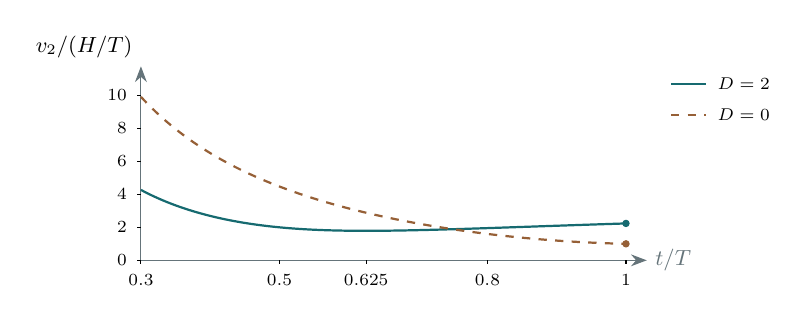
\begin{tikzpicture}[scale=.88,transform shape]
\draw[axis] (0,0.0)--(7.3,0.0) node[right] {$t/T$};
\draw[axis] (0,0)--(0,2.8);
\node[above left] at (0,2.8) {$v_2/(H/T)$};
\draw[thin] (0.000000,0.0)--(0.000000,-0.06);\node[below,font=\scriptsize] at (0.000000,-0.08) {$ 0.3 $};
\draw[thin] (2.000000,0.0)--(2.000000,-0.06);\node[below,font=\scriptsize] at (2.000000,-0.08) {$ 0.5 $};
\draw[thin] (3.250000,0.0)--(3.250000,-0.06);\node[below,font=\scriptsize] at (3.250000,-0.08) {$ 0.625 $};
\draw[thin] (5.000000,0.0)--(5.000000,-0.06);\node[below,font=\scriptsize] at (5.000000,-0.08) {$ 0.8 $};
\draw[thin] (7.000000,0.0)--(7.000000,-0.06);\node[below,font=\scriptsize] at (7.000000,-0.08) {$ 1 $};
\draw[thin] (0,0.000000)--(-.06,0.000000);\node[left,font=\scriptsize] at (-.08,0.000000) {$ 0 $};
\draw[thin] (0,0.476190)--(-.06,0.476190);\node[left,font=\scriptsize] at (-.08,0.476190) {$ 2 $};
\draw[thin] (0,0.952381)--(-.06,0.952381);\node[left,font=\scriptsize] at (-.08,0.952381) {$ 4 $};
\draw[thin] (0,1.428571)--(-.06,1.428571);\node[left,font=\scriptsize] at (-.08,1.428571) {$ 6 $};
\draw[thin] (0,1.904762)--(-.06,1.904762);\node[left,font=\scriptsize] at (-.08,1.904762) {$ 8 $};
\draw[thin] (0,2.380952)--(-.06,2.380952);\node[left,font=\scriptsize] at (-.08,2.380952) {$ 10 $};
\draw[thick,color=accent] plot coordinates {(0.0000000,1.0163689) (0.0291667,1.0008798) (0.0583333,0.9857374) (0.0875000,0.9709329) (0.1166667,0.9564575) (0.1458333,0.9423030) (0.1750000,0.9284615) (0.2041667,0.9149252) (0.2333333,0.9016869) (0.2625000,0.8887394) (0.2916667,0.8760758) (0.3208333,0.8636896) (0.3500000,0.8515745) (0.3791667,0.8397242) (0.4083333,0.8281329) (0.4375000,0.8167949) (0.4666667,0.8057047) (0.4958333,0.7948570) (0.5250000,0.7842466) (0.5541667,0.7738686) (0.5833333,0.7637183) (0.6125000,0.7537909) (0.6416667,0.7440820) (0.6708333,0.7345873) (0.7000000,0.7253026) (0.7291667,0.7162238) (0.7583333,0.7073470) (0.7875000,0.6986684) (0.8166667,0.6901843) (0.8458333,0.6818911) (0.8750000,0.6737853) (0.9041667,0.6658636) (0.9333333,0.6581227) (0.9625000,0.6505594) (0.9916667,0.6431705) (1.0208333,0.6359532) (1.0500000,0.6289044) (1.0791667,0.6220213) (1.1083333,0.6153011) (1.1375000,0.6087411) (1.1666667,0.6023386) (1.1958333,0.5960911) (1.2250000,0.5899960) (1.2541667,0.5840509) (1.2833333,0.5782533) (1.3125000,0.5726009) (1.3416667,0.5670914) (1.3708333,0.5617224) (1.4000000,0.5564918) (1.4291667,0.5513973) (1.4583333,0.5464369) (1.4875000,0.5416083) (1.5166667,0.5369096) (1.5458333,0.5323386) (1.5750000,0.5278934) (1.6041667,0.5235719) (1.6333333,0.5193722) (1.6625000,0.5152924) (1.6916667,0.5113306) (1.7208333,0.5074848) (1.7500000,0.5037532) (1.7791667,0.5001339) (1.8083333,0.4966252) (1.8375000,0.4932252) (1.8666667,0.4899321) (1.8958333,0.4867442) (1.9250000,0.4836596) (1.9541667,0.4806767) (1.9833333,0.4777937) (2.0125000,0.4750089) (2.0416667,0.4723206) (2.0708333,0.4697271) (2.1000000,0.4672267) (2.1291667,0.4648178) (2.1583333,0.4624988) (2.1875000,0.4602678) (2.2166667,0.4581235) (2.2458333,0.4560640) (2.2750000,0.4540879) (2.3041667,0.4521936) (2.3333333,0.4503793) (2.3625000,0.4486437) (2.3916667,0.4469851) (2.4208333,0.4454020) (2.4500000,0.4438929) (2.4791667,0.4424562) (2.5083333,0.4410905) (2.5375000,0.4397942) (2.5666667,0.4385659) (2.5958333,0.4374042) (2.6250000,0.4363075) (2.6541667,0.4352744) (2.6833333,0.4343036) (2.7125000,0.4333936) (2.7416667,0.4325431) (2.7708333,0.4317507) (2.8000000,0.4310149) (2.8291667,0.4303346) (2.8583333,0.4297083) (2.8875000,0.4291349) (2.9166667,0.4286129) (2.9458333,0.4281411) (2.9750000,0.4277184) (3.0041667,0.4273433) (3.0333333,0.4270149) (3.0625000,0.4267317) (3.0916667,0.4264928) (3.1208333,0.4262969) (3.1500000,0.4261429) (3.1791667,0.4260296) (3.2083333,0.4259561) (3.2375000,0.4259211) (3.2666667,0.4259237) (3.2958333,0.4259629) (3.3250000,0.4260375) (3.3541667,0.4261466) (3.3833333,0.4262892) (3.4125000,0.4264644) (3.4416667,0.4266712) (3.4708333,0.4269087) (3.5000000,0.4271760) (3.5291667,0.4274722) (3.5583333,0.4277964) (3.5875000,0.4281478) (3.6166667,0.4285256) (3.6458333,0.4289290) (3.6750000,0.4293571) (3.7041667,0.4298092) (3.7333333,0.4302846) (3.7625000,0.4307824) (3.7916667,0.4313020) (3.8208333,0.4318427) (3.8500000,0.4324038) (3.8791667,0.4329846) (3.9083333,0.4335844) (3.9375000,0.4342027) (3.9666667,0.4348387) (3.9958333,0.4354920) (4.0250000,0.4361618) (4.0541667,0.4368477) (4.0833333,0.4375490) (4.1125000,0.4382652) (4.1416667,0.4389958) (4.1708333,0.4397403) (4.2000000,0.4404980) (4.2291667,0.4412687) (4.2583333,0.4420517) (4.2875000,0.4428466) (4.3166667,0.4436530) (4.3458333,0.4444703) (4.3750000,0.4452983) (4.4041667,0.4461364) (4.4333333,0.4469842) (4.4625000,0.4478414) (4.4916667,0.4487076) (4.5208333,0.4495824) (4.5500000,0.4504654) (4.5791667,0.4513562) (4.6083333,0.4522546) (4.6375000,0.4531602) (4.6666667,0.4540727) (4.6958333,0.4549917) (4.7250000,0.4559170) (4.7541667,0.4568482) (4.7833333,0.4577851) (4.8125000,0.4587274) (4.8416667,0.4596748) (4.8708333,0.4606270) (4.9000000,0.4615838) (4.9291667,0.4625450) (4.9583333,0.4635102) (4.9875000,0.4644794) (5.0166667,0.4654521) (5.0458333,0.4664283) (5.0750000,0.4674076) (5.1041667,0.4683900) (5.1333333,0.4693751) (5.1625000,0.4703628) (5.1916667,0.4713529) (5.2208333,0.4723453) (5.2500000,0.4733397) (5.2791667,0.4743359) (5.3083333,0.4753339) (5.3375000,0.4763333) (5.3666667,0.4773342) (5.3958333,0.4783363) (5.4250000,0.4793395) (5.4541667,0.4803436) (5.4833333,0.4813485) (5.5125000,0.4823540) (5.5416667,0.4833601) (5.5708333,0.4843666) (5.6000000,0.4853734) (5.6291667,0.4863803) (5.6583333,0.4873873) (5.6875000,0.4883942) (5.7166667,0.4894010) (5.7458333,0.4904074) (5.7750000,0.4914135) (5.8041667,0.4924192) (5.8333333,0.4934243) (5.8625000,0.4944287) (5.8916667,0.4954324) (5.9208333,0.4964352) (5.9500000,0.4974372) (5.9791667,0.4984381) (6.0083333,0.4994380) (6.0375000,0.5004368) (6.0666667,0.5014343) (6.0958333,0.5024306) (6.1250000,0.5034255) (6.1541667,0.5044190) (6.1833333,0.5054110) (6.2125000,0.5064015) (6.2416667,0.5073904) (6.2708333,0.5083777) (6.3000000,0.5093632) (6.3291667,0.5103471) (6.3583333,0.5113291) (6.3875000,0.5123092) (6.4166667,0.5132875) (6.4458333,0.5142638) (6.4750000,0.5152381) (6.5041667,0.5162105) (6.5333333,0.5171807) (6.5625000,0.5181489) (6.5916667,0.5191149) (6.6208333,0.5200787) (6.6500000,0.5210403) (6.6791667,0.5219997) (6.7083333,0.5229568) (6.7375000,0.5239117) (6.7666667,0.5248642) (6.7958333,0.5258143) (6.8250000,0.5267620) (6.8541667,0.5277074) (6.8833333,0.5286503) (6.9125000,0.5295907) (6.9416667,0.5305287) (6.9708333,0.5314642) (7.0000000,0.5323971)};
\draw[thick,color=accent] (7.65,2.55)--(8.15,2.55);\node[right,font=\scriptsize] at (8.2,2.55) {$D=2$};
\draw[thick,dashed,color=warm] plot coordinates {(0.0000000,2.3596935) (0.0291667,2.3283391) (0.0583333,2.2975868) (0.0875000,2.2674196) (0.1166667,2.2378211) (0.1458333,2.2087756) (0.1750000,2.1802678) (0.2041667,2.1522832) (0.2333333,2.1248075) (0.2625000,2.0978273) (0.2916667,2.0713293) (0.3208333,2.0453009) (0.3500000,2.0197299) (0.3791667,1.9946046) (0.4083333,1.9699134) (0.4375000,1.9456455) (0.4666667,1.9217901) (0.4958333,1.8983370) (0.5250000,1.8752763) (0.5541667,1.8525983) (0.5833333,1.8302938) (0.6125000,1.8083537) (0.6416667,1.7867694) (0.6708333,1.7655324) (0.7000000,1.7446346) (0.7291667,1.7240680) (0.7583333,1.7038250) (0.7875000,1.6838982) (0.8166667,1.6642804) (0.8458333,1.6449645) (0.8750000,1.6259439) (0.9041667,1.6072120) (0.9333333,1.5887624) (0.9625000,1.5705889) (0.9916667,1.5526855) (1.0208333,1.5350464) (1.0500000,1.5176660) (1.0791667,1.5005388) (1.1083333,1.4836594) (1.1375000,1.4670226) (1.1666667,1.4506234) (1.1958333,1.4344570) (1.2250000,1.4185185) (1.2541667,1.4028033) (1.2833333,1.3873070) (1.3125000,1.3720251) (1.3416667,1.3569534) (1.3708333,1.3420877) (1.4000000,1.3274241) (1.4291667,1.3129585) (1.4583333,1.2986872) (1.4875000,1.2846064) (1.5166667,1.2707125) (1.5458333,1.2570020) (1.5750000,1.2434715) (1.6041667,1.2301175) (1.6333333,1.2169369) (1.6625000,1.2039264) (1.6916667,1.1910829) (1.7208333,1.1784034) (1.7500000,1.1658850) (1.7791667,1.1535248) (1.8083333,1.1413200) (1.8375000,1.1292678) (1.8666667,1.1173656) (1.8958333,1.1056108) (1.9250000,1.0940008) (1.9541667,1.0825331) (1.9833333,1.0712054) (2.0125000,1.0600152) (2.0416667,1.0489603) (2.0708333,1.0380384) (2.1000000,1.0272472) (2.1291667,1.0165848) (2.1583333,1.0060489) (2.1875000,0.9956375) (2.2166667,0.9853487) (2.2458333,0.9751803) (2.2750000,0.9651306) (2.3041667,0.9551977) (2.3333333,0.9453798) (2.3625000,0.9356750) (2.3916667,0.9260816) (2.4208333,0.9165979) (2.4500000,0.9072223) (2.4791667,0.8979531) (2.5083333,0.8887888) (2.5375000,0.8797277) (2.5666667,0.8707683) (2.5958333,0.8619092) (2.6250000,0.8531490) (2.6541667,0.8444861) (2.6833333,0.8359192) (2.7125000,0.8274469) (2.7416667,0.8190679) (2.7708333,0.8107808) (2.8000000,0.8025845) (2.8291667,0.7944777) (2.8583333,0.7864591) (2.8875000,0.7785275) (2.9166667,0.7706818) (2.9458333,0.7629209) (2.9750000,0.7552435) (3.0041667,0.7476487) (3.0333333,0.7401353) (3.0625000,0.7327023) (3.0916667,0.7253487) (3.1208333,0.7180735) (3.1500000,0.7108756) (3.1791667,0.7037542) (3.2083333,0.6967082) (3.2375000,0.6897368) (3.2666667,0.6828391) (3.2958333,0.6760141) (3.3250000,0.6692611) (3.3541667,0.6625791) (3.3833333,0.6559674) (3.4125000,0.6494251) (3.4416667,0.6429514) (3.4708333,0.6365456) (3.5000000,0.6302070) (3.5291667,0.6239347) (3.5583333,0.6177281) (3.5875000,0.6115864) (3.6166667,0.6055090) (3.6458333,0.5994951) (3.6750000,0.5935442) (3.7041667,0.5876556) (3.7333333,0.5818285) (3.7625000,0.5760626) (3.7916667,0.5703570) (3.8208333,0.5647112) (3.8500000,0.5591247) (3.8791667,0.5535969) (3.9083333,0.5481273) (3.9375000,0.5427152) (3.9666667,0.5373602) (3.9958333,0.5320618) (4.0250000,0.5268195) (4.0541667,0.5216327) (4.0833333,0.5165011) (4.1125000,0.5114241) (4.1416667,0.5064013) (4.1708333,0.5014322) (4.2000000,0.4965165) (4.2291667,0.4916537) (4.2583333,0.4868434) (4.2875000,0.4820852) (4.3166667,0.4773787) (4.3458333,0.4727236) (4.3750000,0.4681195) (4.4041667,0.4635659) (4.4333333,0.4590627) (4.4625000,0.4546094) (4.4916667,0.4502058) (4.5208333,0.4458515) (4.5500000,0.4415462) (4.5791667,0.4372895) (4.6083333,0.4330814) (4.6375000,0.4289213) (4.6666667,0.4248092) (4.6958333,0.4207447) (4.7250000,0.4167275) (4.7541667,0.4127575) (4.7833333,0.4088344) (4.8125000,0.4049579) (4.8416667,0.4011279) (4.8708333,0.3973442) (4.9000000,0.3936065) (4.9291667,0.3899146) (4.9583333,0.3862684) (4.9875000,0.3826676) (5.0166667,0.3791122) (5.0458333,0.3756019) (5.0750000,0.3721366) (5.1041667,0.3687162) (5.1333333,0.3653404) (5.1625000,0.3620092) (5.1916667,0.3587224) (5.2208333,0.3554799) (5.2500000,0.3522815) (5.2791667,0.3491273) (5.3083333,0.3460169) (5.3375000,0.3429504) (5.3666667,0.3399277) (5.3958333,0.3369486) (5.4250000,0.3340131) (5.4541667,0.3311210) (5.4833333,0.3282723) (5.5125000,0.3254670) (5.5416667,0.3227049) (5.5708333,0.3199859) (5.6000000,0.3173101) (5.6291667,0.3146772) (5.6583333,0.3120874) (5.6875000,0.3095404) (5.7166667,0.3070364) (5.7458333,0.3045751) (5.7750000,0.3021565) (5.8041667,0.2997806) (5.8333333,0.2974474) (5.8625000,0.2951567) (5.8916667,0.2929085) (5.9208333,0.2907028) (5.9500000,0.2885394) (5.9791667,0.2864185) (6.0083333,0.2843398) (6.0375000,0.2823033) (6.0666667,0.2803089) (6.0958333,0.2783567) (6.1250000,0.2764464) (6.1541667,0.2745782) (6.1833333,0.2727517) (6.2125000,0.2709671) (6.2416667,0.2692241) (6.2708333,0.2675227) (6.3000000,0.2658629) (6.3291667,0.2642444) (6.3583333,0.2626672) (6.3875000,0.2611312) (6.4166667,0.2596363) (6.4458333,0.2581822) (6.4750000,0.2567690) (6.5041667,0.2553963) (6.5333333,0.2540642) (6.5625000,0.2527724) (6.5916667,0.2515207) (6.6208333,0.2503090) (6.6500000,0.2491370) (6.6791667,0.2480047) (6.7083333,0.2469117) (6.7375000,0.2458579) (6.7666667,0.2448430) (6.7958333,0.2438668) (6.8250000,0.2429291) (6.8541667,0.2420296) (6.8833333,0.2411680) (6.9125000,0.2403440) (6.9416667,0.2395575) (6.9708333,0.2388080) (7.0000000,0.2380952)};
\draw[thick,dashed,color=warm] (7.65,2.0999999999999996)--(8.15,2.0999999999999996);\node[right,font=\scriptsize] at (8.2,2.0999999999999996) {$D=0$};
\draw[fill=white,color=accent] (7.0000000,0.5323971) circle(.045);\draw[fill=white,color=warm] (7,0.2380952) circle(.045);
\end{tikzpicture}
\figcaption{解图力试1.1B\quad 时间曲线比较可取极小值与末时刻极限}
\end{minipage}\end{center}
速度平面给出同一求导过程的几何解释。令$s=1/t$，
\[
(u_x,u_y)=(v_1,0)+s(-a,H),\qquad s>1/T.
\]
速度端点从$s=1/T$的空心点$U_T$沿$(-a,H)$方向伸展。由速度原点到整条直线作垂线，垂足$U_*$给整条直线的最短距离。解图力试1.1C左侧的$U_*$位于允许射线内，对应$t_*<T$；右侧的垂足位于射线端点之前，最短可行速度只能趋向端点。
\begin{center}\begin{minipage}{.98\linewidth}\centering
\begin{tikzpicture}[scale=.7,transform shape]
\begin{scope}[shift={(0,0)}]
\draw[axis] (-2.7,0)--(4.7,0) node[right] {$u_x$};\draw[axis] (0,0)--(0,2.2) node[above] {$u_y$};
\draw[guide] (4,0)--(2,1);
\draw[thick,color=accent] plot coordinates {(2.0000000,1.0000000) (1.9900000,1.0050000) (1.9800000,1.0100000) (1.9700000,1.0150000) (1.9600000,1.0200000) (1.9500000,1.0250000) (1.9400000,1.0300000) (1.9300000,1.0350000) (1.9200000,1.0400000) (1.9100000,1.0450000) (1.9000000,1.0500000) (1.8900000,1.0550000) (1.8800000,1.0600000) (1.8700000,1.0650000) (1.8600000,1.0700000) (1.8500000,1.0750000) (1.8400000,1.0800000) (1.8300000,1.0850000) (1.8200000,1.0900000) (1.8100000,1.0950000) (1.8000000,1.1000000) (1.7900000,1.1050000) (1.7800000,1.1100000) (1.7700000,1.1150000) (1.7600000,1.1200000) (1.7500000,1.1250000) (1.7400000,1.1300000) (1.7300000,1.1350000) (1.7200000,1.1400000) (1.7100000,1.1450000) (1.7000000,1.1500000) (1.6900000,1.1550000) (1.6800000,1.1600000) (1.6700000,1.1650000) (1.6600000,1.1700000) (1.6500000,1.1750000) (1.6400000,1.1800000) (1.6300000,1.1850000) (1.6200000,1.1900000) (1.6100000,1.1950000) (1.6000000,1.2000000) (1.5900000,1.2050000) (1.5800000,1.2100000) (1.5700000,1.2150000) (1.5600000,1.2200000) (1.5500000,1.2250000) (1.5400000,1.2300000) (1.5300000,1.2350000) (1.5200000,1.2400000) (1.5100000,1.2450000) (1.5000000,1.2500000) (1.4900000,1.2550000) (1.4800000,1.2600000) (1.4700000,1.2650000) (1.4600000,1.2700000) (1.4500000,1.2750000) (1.4400000,1.2800000) (1.4300000,1.2850000) (1.4200000,1.2900000) (1.4100000,1.2950000) (1.4000000,1.3000000) (1.3900000,1.3050000) (1.3800000,1.3100000) (1.3700000,1.3150000) (1.3600000,1.3200000) (1.3500000,1.3250000) (1.3400000,1.3300000) (1.3300000,1.3350000) (1.3200000,1.3400000) (1.3100000,1.3450000) (1.3000000,1.3500000) (1.2900000,1.3550000) (1.2800000,1.3600000) (1.2700000,1.3650000) (1.2600000,1.3700000) (1.2500000,1.3750000) (1.2400000,1.3800000) (1.2300000,1.3850000) (1.2200000,1.3900000) (1.2100000,1.3950000) (1.2000000,1.4000000) (1.1900000,1.4050000) (1.1800000,1.4100000) (1.1700000,1.4150000) (1.1600000,1.4200000) (1.1500000,1.4250000) (1.1400000,1.4300000) (1.1300000,1.4350000) (1.1200000,1.4400000) (1.1100000,1.4450000) (1.1000000,1.4500000) (1.0900000,1.4550000) (1.0800000,1.4600000) (1.0700000,1.4650000) (1.0600000,1.4700000) (1.0500000,1.4750000) (1.0400000,1.4800000) (1.0300000,1.4850000) (1.0200000,1.4900000) (1.0100000,1.4950000) (1.0000000,1.5000000) (0.9900000,1.5050000) (0.9800000,1.5100000) (0.9700000,1.5150000) (0.9600000,1.5200000) (0.9500000,1.5250000) (0.9400000,1.5300000) (0.9300000,1.5350000) (0.9200000,1.5400000) (0.9100000,1.5450000) (0.9000000,1.5500000) (0.8900000,1.5550000) (0.8800000,1.5600000) (0.8700000,1.5650000) (0.8600000,1.5700000) (0.8500000,1.5750000) (0.8400000,1.5800000) (0.8300000,1.5850000) (0.8200000,1.5900000) (0.8100000,1.5950000) (0.8000000,1.6000000)};
\draw[fill=white] (2,1) circle(.06) node[below right] {$U_T$};
\fill[color=warm] (0.8000000,1.6000000) circle(.045);
\draw[guide] (0,0)--(0.8000000,1.6000000);
\node[above] at (1,2.6) {内点最优：$D=2$};
\node[above right] at (.8,1.6) {$U_*$};
\draw[motion] (.9,1.55)--(.55,1.725);
\end{scope}
\begin{scope}[shift={(8.5,0)}]
\draw[axis] (-2.7,0)--(4.7,0) node[right] {$u_x$};\draw[axis] (0,0)--(0,2.2) node[above] {$u_y$};
\draw[guide] (4,0)--(0,1);
\draw[thick,color=accent] plot coordinates {(0.0000000,1.0000000) (-0.0200000,1.0050000) (-0.0400000,1.0100000) (-0.0600000,1.0150000) (-0.0800000,1.0200000) (-0.1000000,1.0250000) (-0.1200000,1.0300000) (-0.1400000,1.0350000) (-0.1600000,1.0400000) (-0.1800000,1.0450000) (-0.2000000,1.0500000) (-0.2200000,1.0550000) (-0.2400000,1.0600000) (-0.2600000,1.0650000) (-0.2800000,1.0700000) (-0.3000000,1.0750000) (-0.3200000,1.0800000) (-0.3400000,1.0850000) (-0.3600000,1.0900000) (-0.3800000,1.0950000) (-0.4000000,1.1000000) (-0.4200000,1.1050000) (-0.4400000,1.1100000) (-0.4600000,1.1150000) (-0.4800000,1.1200000) (-0.5000000,1.1250000) (-0.5200000,1.1300000) (-0.5400000,1.1350000) (-0.5600000,1.1400000) (-0.5800000,1.1450000) (-0.6000000,1.1500000) (-0.6200000,1.1550000) (-0.6400000,1.1600000) (-0.6600000,1.1650000) (-0.6800000,1.1700000) (-0.7000000,1.1750000) (-0.7200000,1.1800000) (-0.7400000,1.1850000) (-0.7600000,1.1900000) (-0.7800000,1.1950000) (-0.8000000,1.2000000) (-0.8200000,1.2050000) (-0.8400000,1.2100000) (-0.8600000,1.2150000) (-0.8800000,1.2200000) (-0.9000000,1.2250000) (-0.9200000,1.2300000) (-0.9400000,1.2350000) (-0.9600000,1.2400000) (-0.9800000,1.2450000) (-1.0000000,1.2500000) (-1.0200000,1.2550000) (-1.0400000,1.2600000) (-1.0600000,1.2650000) (-1.0800000,1.2700000) (-1.1000000,1.2750000) (-1.1200000,1.2800000) (-1.1400000,1.2850000) (-1.1600000,1.2900000) (-1.1800000,1.2950000) (-1.2000000,1.3000000) (-1.2200000,1.3050000) (-1.2400000,1.3100000) (-1.2600000,1.3150000) (-1.2800000,1.3200000) (-1.3000000,1.3250000) (-1.3200000,1.3300000) (-1.3400000,1.3350000) (-1.3600000,1.3400000) (-1.3800000,1.3450000) (-1.4000000,1.3500000) (-1.4200000,1.3550000) (-1.4400000,1.3600000) (-1.4600000,1.3650000) (-1.4800000,1.3700000) (-1.5000000,1.3750000) (-1.5200000,1.3800000) (-1.5400000,1.3850000) (-1.5600000,1.3900000) (-1.5800000,1.3950000) (-1.6000000,1.4000000) (-1.6200000,1.4050000) (-1.6400000,1.4100000) (-1.6600000,1.4150000) (-1.6800000,1.4200000) (-1.7000000,1.4250000) (-1.7200000,1.4300000) (-1.7400000,1.4350000) (-1.7600000,1.4400000) (-1.7800000,1.4450000) (-1.8000000,1.4500000) (-1.8200000,1.4550000) (-1.8400000,1.4600000) (-1.8600000,1.4650000) (-1.8800000,1.4700000) (-1.9000000,1.4750000) (-1.9200000,1.4800000) (-1.9400000,1.4850000) (-1.9600000,1.4900000) (-1.9800000,1.4950000) (-2.0000000,1.5000000) (-2.0200000,1.5050000) (-2.0400000,1.5100000) (-2.0600000,1.5150000) (-2.0800000,1.5200000) (-2.1000000,1.5250000) (-2.1200000,1.5300000) (-2.1400000,1.5350000) (-2.1600000,1.5400000) (-2.1800000,1.5450000) (-2.2000000,1.5500000) (-2.2200000,1.5550000) (-2.2400000,1.5600000) (-2.2600000,1.5650000) (-2.2800000,1.5700000) (-2.3000000,1.5750000) (-2.3200000,1.5800000) (-2.3400000,1.5850000) (-2.3600000,1.5900000) (-2.3800000,1.5950000) (-2.4000000,1.6000000)};
\draw[fill=white] (0,1) circle(.06) node[below right] {$U_T$};
\fill[color=warm] (0.2352941,0.9411765) circle(.045);
\draw[guide] (0,0)--(0.2352941,0.9411765);
\node[above] at (1,2.6) {末时刻极限：$D=0$};
\draw[guide] (.2352941,.9411765)--(1.2,1.9);\node[above right] at (1.2,1.9) {$U_*$};
\draw[motion] (-2.0,1.5)--(-2.6,1.65);
\end{scope}
\end{tikzpicture}
\figcaption{解图力试1.1C\quad 实线为允许速度射线，空心点为t等于T的极限，U星为整条直线垂足}
\end{minipage}\end{center}
若$D(L-D)\le H^2$，包括$a\le0$及$t_*=T$，则在$0<t<T$中速度持续下降，其下确界为
\[
\inf_{0<t<T}v_2
=\sqrt{F(T)}
=\boxed{\frac{\sqrt{D^2+H^2}}{T}}.
\]
飞行中拦截所需速度严格大于此下界，它在$t\to T^-$时被任意逼近。若将落地瞬间也计入相遇，定义域改为$0<t\le T$，同一数值便在$t=T$取到。两类结果由时间区间的开、闭端点决定。

在可取的内点极小值处，把$t_*$代回两个初速分量，得到
\[
u_{x*}=\frac{v_1H^2}{a^2+H^2},\qquad
u_{y*}=\frac{v_1aH}{a^2+H^2},
\quad
\boxed{\alpha_*=\arctan\frac{L-D}{H}}.
\]
此时$a>0$且$u_{x*},u_{y*}>0$，发射角在第一象限。在其余情形，初速端点趋向$U_T=(D/T,H/T)$，因而极限方向为
\[
\alpha\longrightarrow\operatorname{atan2}(H,D)
\quad(t\to T^-).
\]
例如$D=0$时，炮位就在目标处，极限发射为竖直向上，速度趋向$H/T=\sqrt{gH/2}$；任一$t<T$所需速度更大。两问的方向条件由对应时刻的分量式直接给出。

解图力试1.1D进一步把可取内点最优的位置写成$D$的区间。二次函数$D(L-D)$在$D=L/2$最大，最大值为$L^2/4$。因此存在这种炮位的条件是$L>2H$，即$v_1>\sqrt{2gH}$；两临界位置为
\[
 D_\pm=\frac{L\pm\sqrt{L^2-4H^2}}2,\qquad D_-<D<D_+.
\]
在两个端点处$t_*=T$，仍是末时刻极限。图中的抛物线与水平线$H^2$的交点将可取极小值和仅有下确界的炮位分开，与前面的时间及速度图一致。
\begin{center}\begin{minipage}{.98\linewidth}\centering
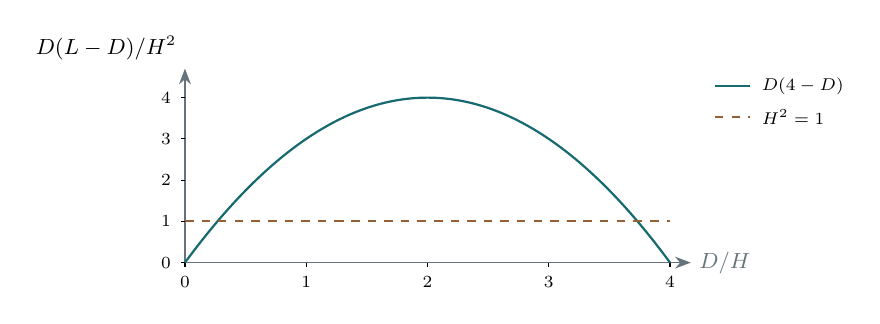
\begin{tikzpicture}[scale=.88,transform shape]
\draw[axis] (0,0.0)--(7.3,0.0) node[right] {$D/H$};
\draw[axis] (0,0)--(0,2.8);
\node[above left] at (0,2.8) {$D(L-D)/H^2$};
\draw[thin] (0.000000,0.0)--(0.000000,-0.06);\node[below,font=\scriptsize] at (0.000000,-0.08) {$ 0 $};
\draw[thin] (1.750000,0.0)--(1.750000,-0.06);\node[below,font=\scriptsize] at (1.750000,-0.08) {$ 1 $};
\draw[thin] (3.500000,0.0)--(3.500000,-0.06);\node[below,font=\scriptsize] at (3.500000,-0.08) {$ 2 $};
\draw[thin] (5.250000,0.0)--(5.250000,-0.06);\node[below,font=\scriptsize] at (5.250000,-0.08) {$ 3 $};
\draw[thin] (7.000000,0.0)--(7.000000,-0.06);\node[below,font=\scriptsize] at (7.000000,-0.08) {$ 4 $};
\draw[thin] (0,0.000000)--(-.06,0.000000);\node[left,font=\scriptsize] at (-.08,0.000000) {$ 0 $};
\draw[thin] (0,0.595238)--(-.06,0.595238);\node[left,font=\scriptsize] at (-.08,0.595238) {$ 1 $};
\draw[thin] (0,1.190476)--(-.06,1.190476);\node[left,font=\scriptsize] at (-.08,1.190476) {$ 2 $};
\draw[thin] (0,1.785714)--(-.06,1.785714);\node[left,font=\scriptsize] at (-.08,1.785714) {$ 3 $};
\draw[thin] (0,2.380952)--(-.06,2.380952);\node[left,font=\scriptsize] at (-.08,2.380952) {$ 4 $};
\draw[thick,color=accent] plot coordinates {(0.0000000,0.0000000) (0.0291667,0.0395172) (0.0583333,0.0787037) (0.0875000,0.1175595) (0.1166667,0.1560847) (0.1458333,0.1942791) (0.1750000,0.2321429) (0.2041667,0.2696759) (0.2333333,0.3068783) (0.2625000,0.3437500) (0.2916667,0.3802910) (0.3208333,0.4165013) (0.3500000,0.4523810) (0.3791667,0.4879299) (0.4083333,0.5231481) (0.4375000,0.5580357) (0.4666667,0.5925926) (0.4958333,0.6268188) (0.5250000,0.6607143) (0.5541667,0.6942791) (0.5833333,0.7275132) (0.6125000,0.7604167) (0.6416667,0.7929894) (0.6708333,0.8252315) (0.7000000,0.8571429) (0.7291667,0.8887235) (0.7583333,0.9199735) (0.7875000,0.9508929) (0.8166667,0.9814815) (0.8458333,1.0117394) (0.8750000,1.0416667) (0.9041667,1.0712632) (0.9333333,1.1005291) (0.9625000,1.1294643) (0.9916667,1.1580688) (1.0208333,1.1863426) (1.0500000,1.2142857) (1.0791667,1.2418981) (1.1083333,1.2691799) (1.1375000,1.2961310) (1.1666667,1.3227513) (1.1958333,1.3490410) (1.2250000,1.3750000) (1.2541667,1.4006283) (1.2833333,1.4259259) (1.3125000,1.4508929) (1.3416667,1.4755291) (1.3708333,1.4998347) (1.4000000,1.5238095) (1.4291667,1.5474537) (1.4583333,1.5707672) (1.4875000,1.5937500) (1.5166667,1.6164021) (1.5458333,1.6387235) (1.5750000,1.6607143) (1.6041667,1.6823743) (1.6333333,1.7037037) (1.6625000,1.7247024) (1.6916667,1.7453704) (1.7208333,1.7657077) (1.7500000,1.7857143) (1.7791667,1.8053902) (1.8083333,1.8247354) (1.8375000,1.8437500) (1.8666667,1.8624339) (1.8958333,1.8807870) (1.9250000,1.8988095) (1.9541667,1.9165013) (1.9833333,1.9338624) (2.0125000,1.9508929) (2.0416667,1.9675926) (2.0708333,1.9839616) (2.1000000,2.0000000) (2.1291667,2.0157077) (2.1583333,2.0310847) (2.1875000,2.0461310) (2.2166667,2.0608466) (2.2458333,2.0752315) (2.2750000,2.0892857) (2.3041667,2.1030093) (2.3333333,2.1164021) (2.3625000,2.1294643) (2.3916667,2.1421958) (2.4208333,2.1545966) (2.4500000,2.1666667) (2.4791667,2.1784061) (2.5083333,2.1898148) (2.5375000,2.2008929) (2.5666667,2.2116402) (2.5958333,2.2220569) (2.6250000,2.2321429) (2.6541667,2.2418981) (2.6833333,2.2513228) (2.7125000,2.2604167) (2.7416667,2.2691799) (2.7708333,2.2776124) (2.8000000,2.2857143) (2.8291667,2.2934854) (2.8583333,2.3009259) (2.8875000,2.3080357) (2.9166667,2.3148148) (2.9458333,2.3212632) (2.9750000,2.3273810) (3.0041667,2.3331680) (3.0333333,2.3386243) (3.0625000,2.3437500) (3.0916667,2.3485450) (3.1208333,2.3530093) (3.1500000,2.3571429) (3.1791667,2.3609458) (3.2083333,2.3644180) (3.2375000,2.3675595) (3.2666667,2.3703704) (3.2958333,2.3728505) (3.3250000,2.3750000) (3.3541667,2.3768188) (3.3833333,2.3783069) (3.4125000,2.3794643) (3.4416667,2.3802910) (3.4708333,2.3807870) (3.5000000,2.3809524) (3.5291667,2.3807870) (3.5583333,2.3802910) (3.5875000,2.3794643) (3.6166667,2.3783069) (3.6458333,2.3768188) (3.6750000,2.3750000) (3.7041667,2.3728505) (3.7333333,2.3703704) (3.7625000,2.3675595) (3.7916667,2.3644180) (3.8208333,2.3609458) (3.8500000,2.3571429) (3.8791667,2.3530093) (3.9083333,2.3485450) (3.9375000,2.3437500) (3.9666667,2.3386243) (3.9958333,2.3331680) (4.0250000,2.3273810) (4.0541667,2.3212632) (4.0833333,2.3148148) (4.1125000,2.3080357) (4.1416667,2.3009259) (4.1708333,2.2934854) (4.2000000,2.2857143) (4.2291667,2.2776124) (4.2583333,2.2691799) (4.2875000,2.2604167) (4.3166667,2.2513228) (4.3458333,2.2418981) (4.3750000,2.2321429) (4.4041667,2.2220569) (4.4333333,2.2116402) (4.4625000,2.2008929) (4.4916667,2.1898148) (4.5208333,2.1784061) (4.5500000,2.1666667) (4.5791667,2.1545966) (4.6083333,2.1421958) (4.6375000,2.1294643) (4.6666667,2.1164021) (4.6958333,2.1030093) (4.7250000,2.0892857) (4.7541667,2.0752315) (4.7833333,2.0608466) (4.8125000,2.0461310) (4.8416667,2.0310847) (4.8708333,2.0157077) (4.9000000,2.0000000) (4.9291667,1.9839616) (4.9583333,1.9675926) (4.9875000,1.9508929) (5.0166667,1.9338624) (5.0458333,1.9165013) (5.0750000,1.8988095) (5.1041667,1.8807870) (5.1333333,1.8624339) (5.1625000,1.8437500) (5.1916667,1.8247354) (5.2208333,1.8053902) (5.2500000,1.7857143) (5.2791667,1.7657077) (5.3083333,1.7453704) (5.3375000,1.7247024) (5.3666667,1.7037037) (5.3958333,1.6823743) (5.4250000,1.6607143) (5.4541667,1.6387235) (5.4833333,1.6164021) (5.5125000,1.5937500) (5.5416667,1.5707672) (5.5708333,1.5474537) (5.6000000,1.5238095) (5.6291667,1.4998347) (5.6583333,1.4755291) (5.6875000,1.4508929) (5.7166667,1.4259259) (5.7458333,1.4006283) (5.7750000,1.3750000) (5.8041667,1.3490410) (5.8333333,1.3227513) (5.8625000,1.2961310) (5.8916667,1.2691799) (5.9208333,1.2418981) (5.9500000,1.2142857) (5.9791667,1.1863426) (6.0083333,1.1580688) (6.0375000,1.1294643) (6.0666667,1.1005291) (6.0958333,1.0712632) (6.1250000,1.0416667) (6.1541667,1.0117394) (6.1833333,0.9814815) (6.2125000,0.9508929) (6.2416667,0.9199735) (6.2708333,0.8887235) (6.3000000,0.8571429) (6.3291667,0.8252315) (6.3583333,0.7929894) (6.3875000,0.7604167) (6.4166667,0.7275132) (6.4458333,0.6942791) (6.4750000,0.6607143) (6.5041667,0.6268188) (6.5333333,0.5925926) (6.5625000,0.5580357) (6.5916667,0.5231481) (6.6208333,0.4879299) (6.6500000,0.4523810) (6.6791667,0.4165013) (6.7083333,0.3802910) (6.7375000,0.3437500) (6.7666667,0.3068783) (6.7958333,0.2696759) (6.8250000,0.2321429) (6.8541667,0.1942791) (6.8833333,0.1560847) (6.9125000,0.1175595) (6.9416667,0.0787037) (6.9708333,0.0395172) (7.0000000,0.0000000)};
\draw[thick,color=accent] (7.65,2.55)--(8.15,2.55);\node[right,font=\scriptsize] at (8.2,2.55) {$D(4-D)$};
\draw[thick,dashed,color=warm] plot coordinates {(0.0000000,0.5952381) (0.0291667,0.5952381) (0.0583333,0.5952381) (0.0875000,0.5952381) (0.1166667,0.5952381) (0.1458333,0.5952381) (0.1750000,0.5952381) (0.2041667,0.5952381) (0.2333333,0.5952381) (0.2625000,0.5952381) (0.2916667,0.5952381) (0.3208333,0.5952381) (0.3500000,0.5952381) (0.3791667,0.5952381) (0.4083333,0.5952381) (0.4375000,0.5952381) (0.4666667,0.5952381) (0.4958333,0.5952381) (0.5250000,0.5952381) (0.5541667,0.5952381) (0.5833333,0.5952381) (0.6125000,0.5952381) (0.6416667,0.5952381) (0.6708333,0.5952381) (0.7000000,0.5952381) (0.7291667,0.5952381) (0.7583333,0.5952381) (0.7875000,0.5952381) (0.8166667,0.5952381) (0.8458333,0.5952381) (0.8750000,0.5952381) (0.9041667,0.5952381) (0.9333333,0.5952381) (0.9625000,0.5952381) (0.9916667,0.5952381) (1.0208333,0.5952381) (1.0500000,0.5952381) (1.0791667,0.5952381) (1.1083333,0.5952381) (1.1375000,0.5952381) (1.1666667,0.5952381) (1.1958333,0.5952381) (1.2250000,0.5952381) (1.2541667,0.5952381) (1.2833333,0.5952381) (1.3125000,0.5952381) (1.3416667,0.5952381) (1.3708333,0.5952381) (1.4000000,0.5952381) (1.4291667,0.5952381) (1.4583333,0.5952381) (1.4875000,0.5952381) (1.5166667,0.5952381) (1.5458333,0.5952381) (1.5750000,0.5952381) (1.6041667,0.5952381) (1.6333333,0.5952381) (1.6625000,0.5952381) (1.6916667,0.5952381) (1.7208333,0.5952381) (1.7500000,0.5952381) (1.7791667,0.5952381) (1.8083333,0.5952381) (1.8375000,0.5952381) (1.8666667,0.5952381) (1.8958333,0.5952381) (1.9250000,0.5952381) (1.9541667,0.5952381) (1.9833333,0.5952381) (2.0125000,0.5952381) (2.0416667,0.5952381) (2.0708333,0.5952381) (2.1000000,0.5952381) (2.1291667,0.5952381) (2.1583333,0.5952381) (2.1875000,0.5952381) (2.2166667,0.5952381) (2.2458333,0.5952381) (2.2750000,0.5952381) (2.3041667,0.5952381) (2.3333333,0.5952381) (2.3625000,0.5952381) (2.3916667,0.5952381) (2.4208333,0.5952381) (2.4500000,0.5952381) (2.4791667,0.5952381) (2.5083333,0.5952381) (2.5375000,0.5952381) (2.5666667,0.5952381) (2.5958333,0.5952381) (2.6250000,0.5952381) (2.6541667,0.5952381) (2.6833333,0.5952381) (2.7125000,0.5952381) (2.7416667,0.5952381) (2.7708333,0.5952381) (2.8000000,0.5952381) (2.8291667,0.5952381) (2.8583333,0.5952381) (2.8875000,0.5952381) (2.9166667,0.5952381) (2.9458333,0.5952381) (2.9750000,0.5952381) (3.0041667,0.5952381) (3.0333333,0.5952381) (3.0625000,0.5952381) (3.0916667,0.5952381) (3.1208333,0.5952381) (3.1500000,0.5952381) (3.1791667,0.5952381) (3.2083333,0.5952381) (3.2375000,0.5952381) (3.2666667,0.5952381) (3.2958333,0.5952381) (3.3250000,0.5952381) (3.3541667,0.5952381) (3.3833333,0.5952381) (3.4125000,0.5952381) (3.4416667,0.5952381) (3.4708333,0.5952381) (3.5000000,0.5952381) (3.5291667,0.5952381) (3.5583333,0.5952381) (3.5875000,0.5952381) (3.6166667,0.5952381) (3.6458333,0.5952381) (3.6750000,0.5952381) (3.7041667,0.5952381) (3.7333333,0.5952381) (3.7625000,0.5952381) (3.7916667,0.5952381) (3.8208333,0.5952381) (3.8500000,0.5952381) (3.8791667,0.5952381) (3.9083333,0.5952381) (3.9375000,0.5952381) (3.9666667,0.5952381) (3.9958333,0.5952381) (4.0250000,0.5952381) (4.0541667,0.5952381) (4.0833333,0.5952381) (4.1125000,0.5952381) (4.1416667,0.5952381) (4.1708333,0.5952381) (4.2000000,0.5952381) (4.2291667,0.5952381) (4.2583333,0.5952381) (4.2875000,0.5952381) (4.3166667,0.5952381) (4.3458333,0.5952381) (4.3750000,0.5952381) (4.4041667,0.5952381) (4.4333333,0.5952381) (4.4625000,0.5952381) (4.4916667,0.5952381) (4.5208333,0.5952381) (4.5500000,0.5952381) (4.5791667,0.5952381) (4.6083333,0.5952381) (4.6375000,0.5952381) (4.6666667,0.5952381) (4.6958333,0.5952381) (4.7250000,0.5952381) (4.7541667,0.5952381) (4.7833333,0.5952381) (4.8125000,0.5952381) (4.8416667,0.5952381) (4.8708333,0.5952381) (4.9000000,0.5952381) (4.9291667,0.5952381) (4.9583333,0.5952381) (4.9875000,0.5952381) (5.0166667,0.5952381) (5.0458333,0.5952381) (5.0750000,0.5952381) (5.1041667,0.5952381) (5.1333333,0.5952381) (5.1625000,0.5952381) (5.1916667,0.5952381) (5.2208333,0.5952381) (5.2500000,0.5952381) (5.2791667,0.5952381) (5.3083333,0.5952381) (5.3375000,0.5952381) (5.3666667,0.5952381) (5.3958333,0.5952381) (5.4250000,0.5952381) (5.4541667,0.5952381) (5.4833333,0.5952381) (5.5125000,0.5952381) (5.5416667,0.5952381) (5.5708333,0.5952381) (5.6000000,0.5952381) (5.6291667,0.5952381) (5.6583333,0.5952381) (5.6875000,0.5952381) (5.7166667,0.5952381) (5.7458333,0.5952381) (5.7750000,0.5952381) (5.8041667,0.5952381) (5.8333333,0.5952381) (5.8625000,0.5952381) (5.8916667,0.5952381) (5.9208333,0.5952381) (5.9500000,0.5952381) (5.9791667,0.5952381) (6.0083333,0.5952381) (6.0375000,0.5952381) (6.0666667,0.5952381) (6.0958333,0.5952381) (6.1250000,0.5952381) (6.1541667,0.5952381) (6.1833333,0.5952381) (6.2125000,0.5952381) (6.2416667,0.5952381) (6.2708333,0.5952381) (6.3000000,0.5952381) (6.3291667,0.5952381) (6.3583333,0.5952381) (6.3875000,0.5952381) (6.4166667,0.5952381) (6.4458333,0.5952381) (6.4750000,0.5952381) (6.5041667,0.5952381) (6.5333333,0.5952381) (6.5625000,0.5952381) (6.5916667,0.5952381) (6.6208333,0.5952381) (6.6500000,0.5952381) (6.6791667,0.5952381) (6.7083333,0.5952381) (6.7375000,0.5952381) (6.7666667,0.5952381) (6.7958333,0.5952381) (6.8250000,0.5952381) (6.8541667,0.5952381) (6.8833333,0.5952381) (6.9125000,0.5952381) (6.9416667,0.5952381) (6.9708333,0.5952381) (7.0000000,0.5952381)};
\draw[thick,dashed,color=warm] (7.65,2.0999999999999996)--(8.15,2.0999999999999996);\node[right,font=\scriptsize] at (8.2,2.0999999999999996) {$H^2=1$};
\end{tikzpicture}
\figcaption{解图力试1.1D\quad 抛物线高于水平线的炮位给落地前内点最优}
\end{minipage}\end{center}


\Needspace{13\baselineskip}

\pdfbookmark[2]{第 2 题 可移动圆环内小球的轨迹与曲率}{q2}

\section*{第 2 题\quad 可移动圆环内小球的轨迹与曲率}\label{q:2}


半径为$R$的竖直空心圆环固定在滑块上，环和滑块总质量为$M$，可在光滑水平地面上平移而不转动。质量为$m$的小球视为质点，可在环内的光滑管道中运动。

开始时环与球都静止，球在最高点。用极小扰动使球向右下滑，讨论扰动趋零时的轨迹。以初始环心$O$为地面坐标原点，水平向右为$x$，竖直向上为$y$。求：
\begin{enumerate}
\item 小球相对地面的轨迹方程。
\item 小球经过圆环右侧点$A$及最低点$B$时，地面轨迹的曲率半径。要求用受力与相对运动说明，而不只引用椭圆曲率公式。
\end{enumerate}


\begin{center}\begin{minipage}{.98\linewidth}\centering
\begin{tikzpicture}[scale=.9,transform shape]
\draw[object] (0.00000,0.00000) circle(3.00000);\draw[object] (-1.50000,-3.10000)--(1.50000,-3.10000)--(1.50000,-3.50000)--(-1.50000,-3.50000)--(-1.50000,-3.10000);\draw[object] (-2.00000,-3.65000)--(2.00000,-3.65000);\draw[object] (-1.00000,-2.82843)--(-1.00000,-3.10000);\draw[object] (1.00000,-2.82843)--(1.00000,-3.10000);\fill (0.00000,3.00000) circle(.035);\node[above] at (0.00000,3.00000) {$m$};\fill (3.00000,0.00000) circle(.035);\node[right] at (3.00000,0.00000) {$A$};\fill (0.00000,-3.00000) circle(.035);\node[above right] at (0.00000,-3.00000) {$B$};\fill (0.00000,0.00000) circle(.035);\node[above left] at (0.00000,0.00000) {$O$};\draw[<->,thin,color=muted] (0.00000,-0.40000)--(3.00000,-0.40000);\node[below] at (1.50000,-0.40000) {$R$};\node[below] at (0.00000,-4.00000) {环与滑块总质量 $M$};
\end{tikzpicture}
\figcaption{图力试1.2\quad 球从环顶向右微扰，A为相对圆的右侧点，B为底点。}
\end{minipage}\end{center}

\Needspace{6\baselineskip}\subsection*{解答}


图力试1.2以初始环心$O$为地面坐标原点，当前环心记为$O'$，其横坐标为$X$，小球地面坐标为$(x,y)$。环与滑块只作水平平移，球和环的相互作用为内力，地面支持力与重力均竖直，故系统水平方向总动量守恒：
\[
m\dot x+M\dot X=0,\qquad mx+MX=0.
\]
第二式由第一式对时间积分，并用初始$x=X=0$确定积分常量。它也说明系统水平质心始终在$O$的竖直线上。相对环心的坐标$(x',y')$与地面坐标之间满足
\[
x'=x-X=\frac{M+m}{M}x,\qquad y'=y.
\]
解图力试1.2A把圆环向左的位移、球对环的横向位移及球对地面的较小横向位移画在一起。相对位置约束$x'^2+y'^2=R^2$于是变成
\[
\boxed{\frac{x^2}{a^2}+\frac{y^2}{R^2}=1},
\qquad a=\frac{M}{M+m}R<R.
\]
轨迹为竖直半长轴$R$、水平半轴$a$的椭圆。记$k=M/(M+m)$，则$a=kR$，$0<k<1$。以从环顶向右量起的角$\theta$为参数，同一位置关系为
\[
x=a\sin\theta,\quad y=R\cos\theta,\quad
X=-\frac{mR}{M+m}\sin\theta.
\]
球向右的相对位移$R\sin\theta$分成球向右的地面位移$kR\sin\theta$和环向左的位移$(1-k)R\sin\theta$，两项相加恢复相对横向距离。
\begin{center}\begin{minipage}{.98\linewidth}\centering
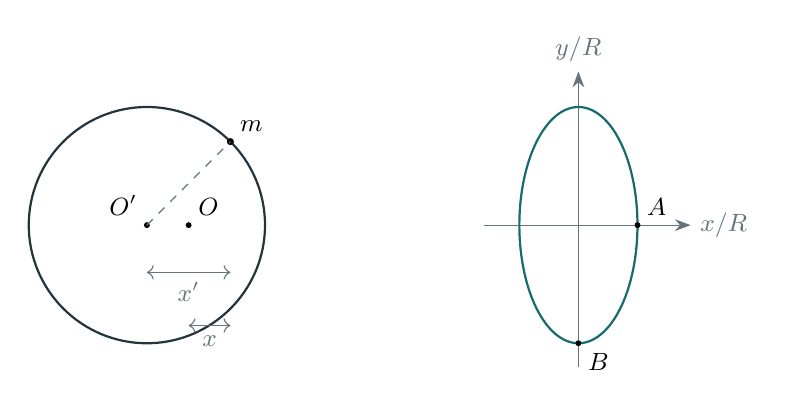
\begin{tikzpicture}[scale=1.5]
\draw[object] (-0.3535534,0) circle(1);
\fill (-0.3535534,0) circle(.025) node[above left] {$O^\prime$};
\fill (0,0) circle(.025) node[above right] {$O$};
\fill (0.3535534,0.7071068) circle(.03) node[above right] {$m$};
\draw[guide] (-0.3535534,0)--(0.3535534,0.7071068);
\draw[<->,thin,color=muted] (-0.3535534,-.4)--(0.3535534,-.4) node[midway,below] {$x^\prime$};
\draw[<->,thin,color=muted] (0,-.85)--(0.3535534,-.85) node[midway,below] {$x$};
\begin{scope}[shift={(3.3,0)}]
\draw[axis] (-.8,0)--(.95,0) node[right] {$x/R$};\draw[axis] (0,-1.2)--(0,1.3) node[above] {$y/R$};
\draw[traj] plot coordinates {(0.0000000,1.0000000) (0.0130885,0.9996573) (0.0261680,0.9986295) (0.0392295,0.9969173) (0.0522642,0.9945219) (0.0652631,0.9914449) (0.0782172,0.9876883) (0.0911178,0.9832549) (0.1039558,0.9781476) (0.1167227,0.9723699) (0.1294095,0.9659258) (0.1420077,0.9588197) (0.1545085,0.9510565) (0.1669034,0.9426415) (0.1791840,0.9335804) (0.1913417,0.9238795) (0.2033683,0.9135455) (0.2152555,0.9025853) (0.2269952,0.8910065) (0.2385794,0.8788171) (0.2500000,0.8660254) (0.2612493,0.8526402) (0.2723195,0.8386706) (0.2832031,0.8241262) (0.2938926,0.8090170) (0.3043807,0.7933533) (0.3146602,0.7771460) (0.3247240,0.7604060) (0.3345653,0.7431448) (0.3441773,0.7253744) (0.3535534,0.7071068) (0.3626872,0.6883546) (0.3715724,0.6691306) (0.3802030,0.6494480) (0.3885730,0.6293204) (0.3966767,0.6087614) (0.4045085,0.5877853) (0.4120631,0.5664062) (0.4193353,0.5446390) (0.4263201,0.5224986) (0.4330127,0.5000000) (0.4394086,0.4771588) (0.4455033,0.4539905) (0.4512926,0.4305111) (0.4567727,0.4067366) (0.4619398,0.3826834) (0.4667902,0.3583679) (0.4713207,0.3338069) (0.4755283,0.3090170) (0.4794099,0.2840153) (0.4829629,0.2588190) (0.4861850,0.2334454) (0.4890738,0.2079117) (0.4916275,0.1822355) (0.4938442,0.1564345) (0.4957224,0.1305262) (0.4972609,0.1045285) (0.4984587,0.0784591) (0.4993148,0.0523360) (0.4998287,0.0261769) (0.5000000,0.0000000) (0.4998287,-0.0261769) (0.4993148,-0.0523360) (0.4984587,-0.0784591) (0.4972609,-0.1045285) (0.4957224,-0.1305262) (0.4938442,-0.1564345) (0.4916275,-0.1822355) (0.4890738,-0.2079117) (0.4861850,-0.2334454) (0.4829629,-0.2588190) (0.4794099,-0.2840153) (0.4755283,-0.3090170) (0.4713207,-0.3338069) (0.4667902,-0.3583679) (0.4619398,-0.3826834) (0.4567727,-0.4067366) (0.4512926,-0.4305111) (0.4455033,-0.4539905) (0.4394086,-0.4771588) (0.4330127,-0.5000000) (0.4263201,-0.5224986) (0.4193353,-0.5446390) (0.4120631,-0.5664062) (0.4045085,-0.5877853) (0.3966767,-0.6087614) (0.3885730,-0.6293204) (0.3802030,-0.6494480) (0.3715724,-0.6691306) (0.3626872,-0.6883546) (0.3535534,-0.7071068) (0.3441773,-0.7253744) (0.3345653,-0.7431448) (0.3247240,-0.7604060) (0.3146602,-0.7771460) (0.3043807,-0.7933533) (0.2938926,-0.8090170) (0.2832031,-0.8241262) (0.2723195,-0.8386706) (0.2612493,-0.8526402) (0.2500000,-0.8660254) (0.2385794,-0.8788171) (0.2269952,-0.8910065) (0.2152555,-0.9025853) (0.2033683,-0.9135455) (0.1913417,-0.9238795) (0.1791840,-0.9335804) (0.1669034,-0.9426415) (0.1545085,-0.9510565) (0.1420077,-0.9588197) (0.1294095,-0.9659258) (0.1167227,-0.9723699) (0.1039558,-0.9781476) (0.0911178,-0.9832549) (0.0782172,-0.9876883) (0.0652631,-0.9914449) (0.0522642,-0.9945219) (0.0392295,-0.9969173) (0.0261680,-0.9986295) (0.0130885,-0.9996573) (0.0000000,-1.0000000) (-0.0130885,-0.9996573) (-0.0261680,-0.9986295) (-0.0392295,-0.9969173) (-0.0522642,-0.9945219) (-0.0652631,-0.9914449) (-0.0782172,-0.9876883) (-0.0911178,-0.9832549) (-0.1039558,-0.9781476) (-0.1167227,-0.9723699) (-0.1294095,-0.9659258) (-0.1420077,-0.9588197) (-0.1545085,-0.9510565) (-0.1669034,-0.9426415) (-0.1791840,-0.9335804) (-0.1913417,-0.9238795) (-0.2033683,-0.9135455) (-0.2152555,-0.9025853) (-0.2269952,-0.8910065) (-0.2385794,-0.8788171) (-0.2500000,-0.8660254) (-0.2612493,-0.8526402) (-0.2723195,-0.8386706) (-0.2832031,-0.8241262) (-0.2938926,-0.8090170) (-0.3043807,-0.7933533) (-0.3146602,-0.7771460) (-0.3247240,-0.7604060) (-0.3345653,-0.7431448) (-0.3441773,-0.7253744) (-0.3535534,-0.7071068) (-0.3626872,-0.6883546) (-0.3715724,-0.6691306) (-0.3802030,-0.6494480) (-0.3885730,-0.6293204) (-0.3966767,-0.6087614) (-0.4045085,-0.5877853) (-0.4120631,-0.5664062) (-0.4193353,-0.5446390) (-0.4263201,-0.5224986) (-0.4330127,-0.5000000) (-0.4394086,-0.4771588) (-0.4455033,-0.4539905) (-0.4512926,-0.4305111) (-0.4567727,-0.4067366) (-0.4619398,-0.3826834) (-0.4667902,-0.3583679) (-0.4713207,-0.3338069) (-0.4755283,-0.3090170) (-0.4794099,-0.2840153) (-0.4829629,-0.2588190) (-0.4861850,-0.2334454) (-0.4890738,-0.2079117) (-0.4916275,-0.1822355) (-0.4938442,-0.1564345) (-0.4957224,-0.1305262) (-0.4972609,-0.1045285) (-0.4984587,-0.0784591) (-0.4993148,-0.0523360) (-0.4998287,-0.0261769) (-0.5000000,-0.0000000) (-0.4998287,0.0261769) (-0.4993148,0.0523360) (-0.4984587,0.0784591) (-0.4972609,0.1045285) (-0.4957224,0.1305262) (-0.4938442,0.1564345) (-0.4916275,0.1822355) (-0.4890738,0.2079117) (-0.4861850,0.2334454) (-0.4829629,0.2588190) (-0.4794099,0.2840153) (-0.4755283,0.3090170) (-0.4713207,0.3338069) (-0.4667902,0.3583679) (-0.4619398,0.3826834) (-0.4567727,0.4067366) (-0.4512926,0.4305111) (-0.4455033,0.4539905) (-0.4394086,0.4771588) (-0.4330127,0.5000000) (-0.4263201,0.5224986) (-0.4193353,0.5446390) (-0.4120631,0.5664062) (-0.4045085,0.5877853) (-0.3966767,0.6087614) (-0.3885730,0.6293204) (-0.3802030,0.6494480) (-0.3715724,0.6691306) (-0.3626872,0.6883546) (-0.3535534,0.7071068) (-0.3441773,0.7253744) (-0.3345653,0.7431448) (-0.3247240,0.7604060) (-0.3146602,0.7771460) (-0.3043807,0.7933533) (-0.2938926,0.8090170) (-0.2832031,0.8241262) (-0.2723195,0.8386706) (-0.2612493,0.8526402) (-0.2500000,0.8660254) (-0.2385794,0.8788171) (-0.2269952,0.8910065) (-0.2152555,0.9025853) (-0.2033683,0.9135455) (-0.1913417,0.9238795) (-0.1791840,0.9335804) (-0.1669034,0.9426415) (-0.1545085,0.9510565) (-0.1420077,0.9588197) (-0.1294095,0.9659258) (-0.1167227,0.9723699) (-0.1039558,0.9781476) (-0.0911178,0.9832549) (-0.0782172,0.9876883) (-0.0652631,0.9914449) (-0.0522642,0.9945219) (-0.0392295,0.9969173) (-0.0261680,0.9986295) (-0.0130885,0.9996573) (-0.0000000,1.0000000)};
\fill (.5,0) circle(.025) node[above right] {$A$};\fill (0,-1) circle(.025) node[below right] {$B$};
\end{scope}
\end{tikzpicture}
\figcaption{解图力试1.2A\quad k等于二分之一的示例：相对圆的横位移分成球与环心的反向位移}
\end{minipage}\end{center}
地面曲率由同一参考系的速度和法向加速度确定。曲线在某点的切线给速度方向，垂直切线的加速度分量满足$a_n=v^2/\rho$；重力及支持力各自在法向上的投影决定该处$a_n$。$A$和$B$两点分别用该瞬间的球、环运动列式，将相对速率换成地面速率。

在解图力试1.2B的右端$A$，$\theta=\pi/2$，球在地面椭圆上的速度竖直向下。由参数式求导，$\dot X=-(1-k)R\cos\theta\,\dot\theta=0$，所以球的地面速率与相对环速率相同，记为$v_A$。球受向左的支持力$N_A$和向下的重力$mg$；前者沿地面曲线法向，后者沿切线。环受到向右的水平反作用力，因而
\[
a_{bx}=-\frac{N_A}{m},\qquad \ddot X=\frac{N_A}{M}.
\]
球相对环沿半径$R$的圆运动，水平方向相对加速度是$-v_A^2/R$。用$a_{bx}-\ddot X=-v_A^2/R$得
\[
N_A\left(\frac1m+\frac1M\right)=\frac{v_A^2}{R},
\quad
N_A=\frac{Mm}{M+m}\frac{v_A^2}{R}.
\]
在随环平移的参考系中，同一关系写成$N_A+m\ddot X=mv_A^2/R$：向左的惯性力$m\ddot X$与支持力共同给相对法向加速度。地面法向加速度为$N_A/m$，故
\[
\boxed{\rho_A=\frac{M+m}{M}R=\frac{R^2}{a}}.
\]
环心瞬时速度虽为零，向右加速度却使球相对环的向左加速度比地面系的大。因此地面轨迹在$A$处比相对圆更平，曲率半径大于$R$，与解图A右端形状一致。
\begin{center}\begin{minipage}{.98\linewidth}\centering
\begin{tikzpicture}[scale=.9,transform shape]
\fill (0,0) circle(.045) node[above right] {$A$};
\draw[force] (0,0)--(-2,0) node[above] {$N_A$};
\draw[force] (0,0)--(0,-1.3) node[left] {$mg$};
\draw[motion] (.7,-.1)--(.7,-1.9) node[right] {$v_A=v_{\rm rel,A}$};
\draw[motion] (2.2,1)--(4.2,1) node[above] {$\ddot X=N_A/M$};
\node[above] at (-.4,1) {球的法向向左};\node at (3.2,.2) {环心瞬时速度为零};
\end{tikzpicture}
\figcaption{解图力试1.2B\quad A处重力沿切线，球与环的水平加速度相反}
\end{minipage}\end{center}
在解图力试1.2C的最低点$B$，$\theta=\pi$，球向左、环心向右运动。设地面速率分别为$v_B$和$V_B$。球所受支持力、重力都竖直，环所受球的反作用力也竖直；水平方向反作用力为零，使$\ddot X=0$。水平动量守恒和速度相减给
\[
MV_B=mv_B,\qquad
v_{\mathrm{rel},B}=v_B+V_B=\frac{M+m}{M}v_B.
\]
相对速率是两相反方向地面速率之和。此时地面曲线与相对圆的切线都水平、法向都竖直；又因环无竖直运动，两个系的竖直加速度相同，所以
\[
N_B-mg=m\frac{v_B^2}{\rho_B}
=m\frac{v_{\mathrm{rel},B}^2}{R}.
\]
相同法向加速度对应不同速率，消去支持力后得
\[
\boxed{\rho_B=\left(\frac{M}{M+m}\right)^2R=\frac{a^2}{R}}.
\]
也可直接由两式相除写成$\rho_B=R(v_B/v_{\rm rel,B})^2=k^2R$。$B$处的环心加速度为零而速度为正，速率换算使椭圆底部的地面曲率半径小于$R$。$A$处处理相对加速度，$B$处处理相对速度，二者由各自受力方向与运动瞬间决定。
\begin{center}\begin{minipage}{.98\linewidth}\centering
\begin{tikzpicture}[scale=.9,transform shape]
\draw[guide] (0,2) circle(2);
\fill (0,0) circle(.045) node[below left] {$B$};
\draw[force] (0,0)--(0,1.5) node[right] {$N_B$};
\draw[force] (0,0)--(0,-1.2) node[right] {$mg$};
\draw[motion] (0,-.25)--(-2,-.25) node[above] {$v_B$};
\fill (0,2) circle(.03) node[above left] {$O^\prime$};
\draw[motion] (0,2)--(1.6,2) node[above] {$V_B$};
\node[right] at (2.2,.6) {$v_{\rm rel,B}=v_B+V_B$};\node[right] at (2.2,1.3) {$\ddot X=0$};
\end{tikzpicture}
\figcaption{解图力试1.2C\quad B处两地面速度反向，相对速率为两者之和}
\end{minipage}\end{center}
椭圆参数式还把两个特殊点连成完整的曲率变化。对$\theta$求导有$x_\theta=a\cos\theta$、$y_\theta=-R\sin\theta$、$x_{\theta\theta}=-a\sin\theta$、$y_{\theta\theta}=-R\cos\theta$，行列式绝对值为$aR$，从而
\[
\rho(\theta)=
\frac{(a^2\cos^2\theta+R^2\sin^2\theta)^{3/2}}{aR}.
\]
解图力试1.2D画$\rho/R$随$\theta$的变化，$\theta=\pi/2,\pi$分别回到$R^2/a$和$a^2/R$。这些半径只含质量比与几何量；重力决定小球怎样随时间经过曲线，求$v^2/a_n$时同一速率尺度相消。$M$很大时$k\to1$，地面椭圆趋近圆，两处半径均趋于$R$；减小$M$使横轴收缩，右端更平而底部更尖。
\begin{center}\begin{minipage}{.98\linewidth}\centering
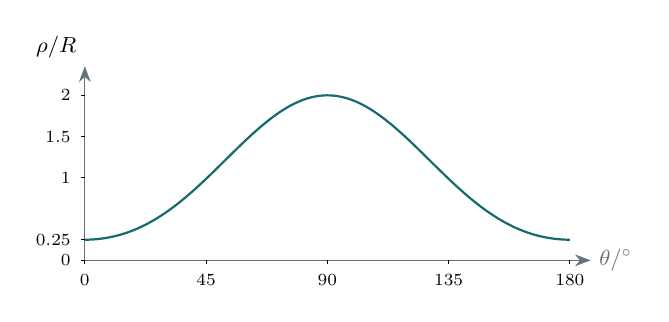
\begin{tikzpicture}[scale=.88,transform shape]
\draw[axis] (0,0.0)--(7.3,0.0) node[right] {$\theta/{}^\circ$};
\draw[axis] (0,0)--(0,2.8);
\node[above left] at (0,2.8) {$\rho/R$};
\draw[thin] (0.000000,0.0)--(0.000000,-0.06);\node[below,font=\scriptsize] at (0.000000,-0.08) {$ 0 $};
\draw[thin] (1.750000,0.0)--(1.750000,-0.06);\node[below,font=\scriptsize] at (1.750000,-0.08) {$ 45 $};
\draw[thin] (3.500000,0.0)--(3.500000,-0.06);\node[below,font=\scriptsize] at (3.500000,-0.08) {$ 90 $};
\draw[thin] (5.250000,0.0)--(5.250000,-0.06);\node[below,font=\scriptsize] at (5.250000,-0.08) {$ 135 $};
\draw[thin] (7.000000,0.0)--(7.000000,-0.06);\node[below,font=\scriptsize] at (7.000000,-0.08) {$ 180 $};
\draw[thin] (0,0.000000)--(-.06,0.000000);\node[left,font=\scriptsize] at (-.08,0.000000) {$ 0 $};
\draw[thin] (0,0.297619)--(-.06,0.297619);\node[left,font=\scriptsize] at (-.08,0.297619) {$ 0.25 $};
\draw[thin] (0,1.190476)--(-.06,1.190476);\node[left,font=\scriptsize] at (-.08,1.190476) {$ 1 $};
\draw[thin] (0,1.785714)--(-.06,1.785714);\node[left,font=\scriptsize] at (-.08,1.785714) {$ 1.5 $};
\draw[thin] (0,2.380952)--(-.06,2.380952);\node[left,font=\scriptsize] at (-.08,2.380952) {$ 2 $};
\draw[thick,color=accent] plot coordinates {(0.0000000,0.2976190) (0.0291667,0.2978485) (0.0583333,0.2985372) (0.0875000,0.2996857) (0.1166667,0.3012949) (0.1458333,0.3033663) (0.1750000,0.3059014) (0.2041667,0.3089024) (0.2333333,0.3123716) (0.2625000,0.3163117) (0.2916667,0.3207257) (0.3208333,0.3256167) (0.3500000,0.3309881) (0.3791667,0.3368435) (0.4083333,0.3431865) (0.4375000,0.3500211) (0.4666667,0.3573509) (0.4958333,0.3651800) (0.5250000,0.3735122) (0.5541667,0.3823513) (0.5833333,0.3917009) (0.6125000,0.4015646) (0.6416667,0.4119458) (0.6708333,0.4228475) (0.7000000,0.4342727) (0.7291667,0.4462238) (0.7583333,0.4587031) (0.7875000,0.4717124) (0.8166667,0.4852532) (0.8458333,0.4993262) (0.8750000,0.5139321) (0.9041667,0.5290707) (0.9333333,0.5447416) (0.9625000,0.5609434) (0.9916667,0.5776746) (1.0208333,0.5949326) (1.0500000,0.6127145) (1.0791667,0.6310167) (1.1083333,0.6498348) (1.1375000,0.6691637) (1.1666667,0.6889977) (1.1958333,0.7093305) (1.2250000,0.7301547) (1.2541667,0.7514625) (1.2833333,0.7732452) (1.3125000,0.7954935) (1.3416667,0.8181972) (1.3708333,0.8413454) (1.4000000,0.8649265) (1.4291667,0.8889281) (1.4583333,0.9133371) (1.4875000,0.9381397) (1.5166667,0.9633212) (1.5458333,0.9888666) (1.5750000,1.0147597) (1.6041667,1.0409839) (1.6333333,1.0675219) (1.6625000,1.0943557) (1.6916667,1.1214667) (1.7208333,1.1488356) (1.7500000,1.1764426) (1.7791667,1.2042672) (1.8083333,1.2322886) (1.8375000,1.2604851) (1.8666667,1.2888347) (1.8958333,1.3173150) (1.9250000,1.3459030) (1.9541667,1.3745752) (1.9833333,1.4033080) (2.0125000,1.4320772) (2.0416667,1.4608582) (2.0708333,1.4896263) (2.1000000,1.5183564) (2.1291667,1.5470232) (2.1583333,1.5756011) (2.1875000,1.6040646) (2.2166667,1.6323876) (2.2458333,1.6605443) (2.2750000,1.6885087) (2.3041667,1.7162547) (2.3333333,1.7437562) (2.3625000,1.7709872) (2.3916667,1.7979218) (2.4208333,1.8245340) (2.4500000,1.8507982) (2.4791667,1.8766889) (2.5083333,1.9021807) (2.5375000,1.9272485) (2.5666667,1.9518675) (2.5958333,1.9760133) (2.6250000,1.9996616) (2.6541667,2.0227888) (2.6833333,2.0453716) (2.7125000,2.0673870) (2.7416667,2.0888126) (2.7708333,2.1096265) (2.8000000,2.1298074) (2.8291667,2.1493346) (2.8583333,2.1681878) (2.8875000,2.1863476) (2.9166667,2.2037950) (2.9458333,2.2205119) (2.9750000,2.2364809) (3.0041667,2.2516851) (3.0333333,2.2661087) (3.0625000,2.2797363) (3.0916667,2.2925538) (3.1208333,2.3045475) (3.1500000,2.3157048) (3.1791667,2.3260137) (3.2083333,2.3354634) (3.2375000,2.3440438) (3.2666667,2.3517458) (3.2958333,2.3585612) (3.3250000,2.3644826) (3.3541667,2.3695038) (3.3833333,2.3736194) (3.4125000,2.3768250) (3.4416667,2.3791172) (3.4708333,2.3804935) (3.5000000,2.3809524) (3.5291667,2.3804935) (3.5583333,2.3791172) (3.5875000,2.3768250) (3.6166667,2.3736194) (3.6458333,2.3695038) (3.6750000,2.3644826) (3.7041667,2.3585612) (3.7333333,2.3517458) (3.7625000,2.3440438) (3.7916667,2.3354634) (3.8208333,2.3260137) (3.8500000,2.3157048) (3.8791667,2.3045475) (3.9083333,2.2925538) (3.9375000,2.2797363) (3.9666667,2.2661087) (3.9958333,2.2516851) (4.0250000,2.2364809) (4.0541667,2.2205119) (4.0833333,2.2037950) (4.1125000,2.1863476) (4.1416667,2.1681878) (4.1708333,2.1493346) (4.2000000,2.1298074) (4.2291667,2.1096265) (4.2583333,2.0888126) (4.2875000,2.0673870) (4.3166667,2.0453716) (4.3458333,2.0227888) (4.3750000,1.9996616) (4.4041667,1.9760133) (4.4333333,1.9518675) (4.4625000,1.9272485) (4.4916667,1.9021807) (4.5208333,1.8766889) (4.5500000,1.8507982) (4.5791667,1.8245340) (4.6083333,1.7979218) (4.6375000,1.7709872) (4.6666667,1.7437562) (4.6958333,1.7162547) (4.7250000,1.6885087) (4.7541667,1.6605443) (4.7833333,1.6323876) (4.8125000,1.6040646) (4.8416667,1.5756011) (4.8708333,1.5470232) (4.9000000,1.5183564) (4.9291667,1.4896263) (4.9583333,1.4608582) (4.9875000,1.4320772) (5.0166667,1.4033080) (5.0458333,1.3745752) (5.0750000,1.3459030) (5.1041667,1.3173150) (5.1333333,1.2888347) (5.1625000,1.2604851) (5.1916667,1.2322886) (5.2208333,1.2042672) (5.2500000,1.1764426) (5.2791667,1.1488356) (5.3083333,1.1214667) (5.3375000,1.0943557) (5.3666667,1.0675219) (5.3958333,1.0409839) (5.4250000,1.0147597) (5.4541667,0.9888666) (5.4833333,0.9633212) (5.5125000,0.9381397) (5.5416667,0.9133371) (5.5708333,0.8889281) (5.6000000,0.8649265) (5.6291667,0.8413454) (5.6583333,0.8181972) (5.6875000,0.7954935) (5.7166667,0.7732452) (5.7458333,0.7514625) (5.7750000,0.7301547) (5.8041667,0.7093305) (5.8333333,0.6889977) (5.8625000,0.6691637) (5.8916667,0.6498348) (5.9208333,0.6310167) (5.9500000,0.6127145) (5.9791667,0.5949326) (6.0083333,0.5776746) (6.0375000,0.5609434) (6.0666667,0.5447416) (6.0958333,0.5290707) (6.1250000,0.5139321) (6.1541667,0.4993262) (6.1833333,0.4852532) (6.2125000,0.4717124) (6.2416667,0.4587031) (6.2708333,0.4462238) (6.3000000,0.4342727) (6.3291667,0.4228475) (6.3583333,0.4119458) (6.3875000,0.4015646) (6.4166667,0.3917009) (6.4458333,0.3823513) (6.4750000,0.3735122) (6.5041667,0.3651800) (6.5333333,0.3573509) (6.5625000,0.3500211) (6.5916667,0.3431865) (6.6208333,0.3368435) (6.6500000,0.3309881) (6.6791667,0.3256167) (6.7083333,0.3207257) (6.7375000,0.3163117) (6.7666667,0.3123716) (6.7958333,0.3089024) (6.8250000,0.3059014) (6.8541667,0.3033663) (6.8833333,0.3012949) (6.9125000,0.2996857) (6.9416667,0.2985372) (6.9708333,0.2978485) (7.0000000,0.2976190)};
\end{tikzpicture}
\figcaption{解图力试1.2D\quad k等于二分之一时地面椭圆的曲率半径}
\end{minipage}\end{center}
题设取最高点微扰趋零的轨迹。最高点完全静止的状态本身是平衡解；微小向右偏离选出下滑方向，得到上面的椭圆轨迹极限。初始时间尺度可随扰动变小而增长，空间轨迹、$A,B$处的速率比与曲率结果保持上述极限。


\Needspace{13\baselineskip}

\pdfbookmark[2]{第 3 题 螺旋槽内下滑与圆筒的平移、自转}{q3}

\section*{第 3 题\quad 螺旋槽内下滑与圆筒的平移、自转}\label{q:3}


质量为$M$、半径为$R$的均匀薄壁圆筒竖直放在光滑水平面上，可水平平移并绕竖直轴自转，保持竖直而不倾倒。筒内壁有一条光滑螺旋槽，筒高$h$恰等于螺距，即沿槽绕筒一周恰从顶端到达底端。小球质量为$m$，从槽顶与圆筒一同静止开始下滑。
\begin{enumerate}
\item 说明下滑过程中圆筒轴线的水平运动与圆筒自转。
\item 求小球从槽顶到槽底相对地面走过的总路程。
\end{enumerate}
圆筒绕自身竖直轴的转动惯量为$I=MR^2$。忽略摩擦和小球尺寸。


\begin{center}\begin{minipage}{.98\linewidth}\centering
\begin{tikzpicture}[scale=.9,transform shape]
\draw[object] plot coordinates {(2.00000,0.00000) (1.99822,0.01897) (1.99289,0.03791) (1.98402,0.05678) (1.97162,0.07554) (1.95571,0.09418) (1.93632,0.11265) (1.91350,0.13091) (1.88727,0.14895) (1.85768,0.16671) (1.82480,0.18419) (1.78866,0.20133) (1.74935,0.21812) (1.70693,0.23452) (1.66147,0.25050) (1.61306,0.26604) (1.56178,0.28110) (1.50773,0.29566) (1.45099,0.30970) (1.39167,0.32319) (1.32988,0.33610) (1.26573,0.34842) (1.19932,0.36011) (1.13078,0.37117) (1.06024,0.38157) (0.98780,0.39128) (0.91361,0.40030) (0.83780,0.40861) (0.76049,0.41620) (0.68184,0.42304) (0.60197,0.42913) (0.52103,0.43446) (0.43917,0.43902) (0.35652,0.44279) (0.27324,0.44578) (0.18948,0.44798) (0.10537,0.44937) (0.02108,0.44997) (-0.06324,0.44977) (-0.14746,0.44878) (-0.23141,0.44698) (-0.31495,0.44439) (-0.39793,0.44100) (-0.48021,0.43684) (-0.56163,0.43189) (-0.64205,0.42618) (-0.72133,0.41971) (-0.79932,0.41250) (-0.87590,0.40455) (-0.95092,0.39588) (-1.02425,0.38651) (-1.09575,0.37645) (-1.16531,0.36572) (-1.23280,0.35435) (-1.29809,0.34234) (-1.36108,0.32972) (-1.42165,0.31652) (-1.47969,0.30275) (-1.53510,0.28845) (-1.58778,0.27363) (-1.63763,0.25833) (-1.68458,0.24256) (-1.72853,0.22637) (-1.76940,0.20977) (-1.80713,0.19280) (-1.84165,0.17549) (-1.87289,0.15786) (-1.90081,0.13996) (-1.92534,0.12181) (-1.94645,0.10344) (-1.96410,0.08488) (-1.97826,0.06618) (-1.98890,0.04735) (-1.99600,0.02845) (-1.99956,0.00949) (-1.99956,-0.00949) (-1.99600,-0.02845) (-1.98890,-0.04735) (-1.97826,-0.06618) (-1.96410,-0.08488) (-1.94645,-0.10344) (-1.92534,-0.12181) (-1.90081,-0.13996) (-1.87289,-0.15786) (-1.84165,-0.17549) (-1.80713,-0.19280) (-1.76940,-0.20977) (-1.72853,-0.22637) (-1.68458,-0.24256) (-1.63763,-0.25833) (-1.58778,-0.27363) (-1.53510,-0.28845) (-1.47969,-0.30275) (-1.42165,-0.31652) (-1.36108,-0.32972) (-1.29809,-0.34234) (-1.23280,-0.35435) (-1.16531,-0.36572) (-1.09575,-0.37645) (-1.02425,-0.38651) (-0.95092,-0.39588) (-0.87590,-0.40455) (-0.79932,-0.41250) (-0.72133,-0.41971) (-0.64205,-0.42618) (-0.56163,-0.43189) (-0.48021,-0.43684) (-0.39793,-0.44100) (-0.31495,-0.44439) (-0.23141,-0.44698) (-0.14746,-0.44878) (-0.06324,-0.44977) (0.02108,-0.44997) (0.10537,-0.44937) (0.18948,-0.44798) (0.27324,-0.44578) (0.35652,-0.44279) (0.43917,-0.43902) (0.52103,-0.43446) (0.60197,-0.42913) (0.68184,-0.42304) (0.76049,-0.41620) (0.83780,-0.40861) (0.91361,-0.40030) (0.98780,-0.39128) (1.06024,-0.38157) (1.13078,-0.37117) (1.19932,-0.36011) (1.26573,-0.34842) (1.32988,-0.33610) (1.39167,-0.32319) (1.45099,-0.30970) (1.50773,-0.29566) (1.56178,-0.28110) (1.61306,-0.26604) (1.66147,-0.25050) (1.70693,-0.23452) (1.74935,-0.21812) (1.78866,-0.20133) (1.82480,-0.18419) (1.85768,-0.16671) (1.88727,-0.14895) (1.91350,-0.13091) (1.93632,-0.11265) (1.95571,-0.09418) (1.97162,-0.07554) (1.98402,-0.05678) (1.99289,-0.03791) (1.99822,-0.01897) (2.00000,-0.00000)};\draw[object] plot coordinates {(2.00000,5.00000) (1.99822,5.01897) (1.99289,5.03791) (1.98402,5.05678) (1.97162,5.07554) (1.95571,5.09418) (1.93632,5.11265) (1.91350,5.13091) (1.88727,5.14895) (1.85768,5.16671) (1.82480,5.18419) (1.78866,5.20133) (1.74935,5.21812) (1.70693,5.23452) (1.66147,5.25050) (1.61306,5.26604) (1.56178,5.28110) (1.50773,5.29566) (1.45099,5.30970) (1.39167,5.32319) (1.32988,5.33610) (1.26573,5.34842) (1.19932,5.36011) (1.13078,5.37117) (1.06024,5.38157) (0.98780,5.39128) (0.91361,5.40030) (0.83780,5.40861) (0.76049,5.41620) (0.68184,5.42304) (0.60197,5.42913) (0.52103,5.43446) (0.43917,5.43902) (0.35652,5.44279) (0.27324,5.44578) (0.18948,5.44798) (0.10537,5.44937) (0.02108,5.44997) (-0.06324,5.44977) (-0.14746,5.44878) (-0.23141,5.44698) (-0.31495,5.44439) (-0.39793,5.44100) (-0.48021,5.43684) (-0.56163,5.43189) (-0.64205,5.42618) (-0.72133,5.41971) (-0.79932,5.41250) (-0.87590,5.40455) (-0.95092,5.39588) (-1.02425,5.38651) (-1.09575,5.37645) (-1.16531,5.36572) (-1.23280,5.35435) (-1.29809,5.34234) (-1.36108,5.32972) (-1.42165,5.31652) (-1.47969,5.30275) (-1.53510,5.28845) (-1.58778,5.27363) (-1.63763,5.25833) (-1.68458,5.24256) (-1.72853,5.22637) (-1.76940,5.20977) (-1.80713,5.19280) (-1.84165,5.17549) (-1.87289,5.15786) (-1.90081,5.13996) (-1.92534,5.12181) (-1.94645,5.10344) (-1.96410,5.08488) (-1.97826,5.06618) (-1.98890,5.04735) (-1.99600,5.02845) (-1.99956,5.00949) (-1.99956,4.99051) (-1.99600,4.97155) (-1.98890,4.95265) (-1.97826,4.93382) (-1.96410,4.91512) (-1.94645,4.89656) (-1.92534,4.87819) (-1.90081,4.86004) (-1.87289,4.84214) (-1.84165,4.82451) (-1.80713,4.80720) (-1.76940,4.79023) (-1.72853,4.77363) (-1.68458,4.75744) (-1.63763,4.74167) (-1.58778,4.72637) (-1.53510,4.71155) (-1.47969,4.69725) (-1.42165,4.68348) (-1.36108,4.67028) (-1.29809,4.65766) (-1.23280,4.64565) (-1.16531,4.63428) (-1.09575,4.62355) (-1.02425,4.61349) (-0.95092,4.60412) (-0.87590,4.59545) (-0.79932,4.58750) (-0.72133,4.58029) (-0.64205,4.57382) (-0.56163,4.56811) (-0.48021,4.56316) (-0.39793,4.55900) (-0.31495,4.55561) (-0.23141,4.55302) (-0.14746,4.55122) (-0.06324,4.55023) (0.02108,4.55003) (0.10537,4.55063) (0.18948,4.55202) (0.27324,4.55422) (0.35652,4.55721) (0.43917,4.56098) (0.52103,4.56554) (0.60197,4.57087) (0.68184,4.57696) (0.76049,4.58380) (0.83780,4.59139) (0.91361,4.59970) (0.98780,4.60872) (1.06024,4.61843) (1.13078,4.62883) (1.19932,4.63989) (1.26573,4.65158) (1.32988,4.66390) (1.39167,4.67681) (1.45099,4.69030) (1.50773,4.70434) (1.56178,4.71890) (1.61306,4.73396) (1.66147,4.74950) (1.70693,4.76548) (1.74935,4.78188) (1.78866,4.79867) (1.82480,4.81581) (1.85768,4.83329) (1.88727,4.85105) (1.91350,4.86909) (1.93632,4.88735) (1.95571,4.90582) (1.97162,4.92446) (1.98402,4.94322) (1.99289,4.96209) (1.99822,4.98103) (2.00000,5.00000)};\draw[object] (-2.00000,0.00000)--(-2.00000,5.00000);\draw[object] (2.00000,0.00000)--(2.00000,5.00000);\draw[traj] plot coordinates {(2.00000,5.00000) (1.99918,4.99008) (1.99671,4.98015) (1.99260,4.97019) (1.98684,4.96021) (1.97946,4.95018) (1.97044,4.94010) (1.95980,4.92995) (1.94755,4.91973) (1.93370,4.90943) (1.91825,4.89903) (1.90122,4.88853) (1.88263,4.87791) (1.86250,4.86717) (1.84082,4.85629) (1.81764,4.84527) (1.79295,4.83409) (1.76679,4.82275) (1.73918,4.81124) (1.71013,4.79954) (1.67968,4.78765) (1.64785,4.77556) (1.61465,4.76326) (1.58013,4.75075) (1.54431,4.73800) (1.50722,4.72502) (1.46889,4.71179) (1.42935,4.69832) (1.38863,4.68458) (1.34677,4.67058) (1.30380,4.65631) (1.25976,4.64175) (1.21468,4.62691) (1.16860,4.61177) (1.12156,4.59633) (1.07359,4.58058) (1.02474,4.56453) (0.97505,4.54815) (0.92456,4.53145) (0.87330,4.51442) (0.82133,4.49706) (0.76868,4.47936) (0.71540,4.46132) (0.66153,4.44294) (0.60711,4.42420) (0.55219,4.40511) (0.49682,4.38567) (0.44105,4.36586) (0.38490,4.34570) (0.32844,4.32517) (0.27172,4.30428) (0.21476,4.28301) (0.15763,4.26139) (0.10037,4.23939) (0.04303,4.21702) (-0.01435,4.19428) (-0.07171,4.17117) (-0.12902,4.14769) (-0.18622,4.12384) (-0.24326,4.09963) (-0.30011,4.07504) (-0.35671,4.05009) (-0.41302,4.02478) (-0.46898,3.99910) (-0.52456,3.97306) (-0.57971,3.94666) (-0.63438,3.91991) (-0.68853,3.89281) (-0.74211,3.86536) (-0.79509,3.83757) (-0.84740,3.80944) (-0.89902,3.78097) (-0.94990,3.75217) (-1.00000,3.72304) (-1.04927,3.69360) (-1.09769,3.66384) (-1.14519,3.63377) (-1.19176,3.60339) (-1.23734,3.57272) (-1.28191,3.54176) (-1.32542,3.51051) (-1.36784,3.47899) (-1.40913,3.44719) (-1.44927,3.41513) (-1.48821,3.38282) (-1.52592,3.35026) (-1.56238,3.31746) (-1.59756,3.28443) (-1.63142,3.25118) (-1.66393,3.21771) (-1.69508,3.18403) (-1.72483,3.15016) (-1.75317,3.11611) (-1.78006,3.08187) (-1.80548,3.04747) (-1.82942,3.01290) (-1.85185,2.97819) (-1.87276,2.94333) (-1.89212,2.90835) (-1.90993,2.87325) (-1.92617,2.83803) (-1.94082,2.80272) (-1.95388,2.76732) (-1.96532,2.73184) (-1.97515,2.69629) (-1.98335,2.66068) (-1.98993,2.62502) (-1.99486,2.58933) (-1.99815,2.55361) (-1.99979,2.51787) (-1.99979,2.48213) (-1.99815,2.44639) (-1.99486,2.41067) (-1.98993,2.37498) (-1.98335,2.33932) (-1.97515,2.30371) (-1.96532,2.26816) (-1.95388,2.23268) (-1.94082,2.19728) (-1.92617,2.16197) (-1.90993,2.12675) (-1.89212,2.09165) (-1.87276,2.05667) (-1.85185,2.02181) (-1.82942,1.98710) (-1.80548,1.95253) (-1.78006,1.91813) (-1.75317,1.88389) (-1.72483,1.84984) (-1.69508,1.81597) (-1.66393,1.78229) (-1.63142,1.74882) (-1.59756,1.71557) (-1.56238,1.68254) (-1.52592,1.64974) (-1.48821,1.61718) (-1.44927,1.58487) (-1.40913,1.55281) (-1.36784,1.52101) (-1.32542,1.48949) (-1.28191,1.45824) (-1.23734,1.42728) (-1.19176,1.39661) (-1.14519,1.36623) (-1.09769,1.33616) (-1.04927,1.30640) (-1.00000,1.27696) (-0.94990,1.24783) (-0.89902,1.21903) (-0.84740,1.19056) (-0.79509,1.16243) (-0.74211,1.13464) (-0.68853,1.10719) (-0.63438,1.08009) (-0.57971,1.05334) (-0.52456,1.02694) (-0.46898,1.00090) (-0.41302,0.97522) (-0.35671,0.94991) (-0.30011,0.92496) (-0.24326,0.90037) (-0.18622,0.87616) (-0.12902,0.85231) (-0.07171,0.82883) (-0.01435,0.80572) (0.04303,0.78298) (0.10037,0.76061) (0.15763,0.73861) (0.21476,0.71699) (0.27172,0.69572) (0.32844,0.67483) (0.38490,0.65430) (0.44105,0.63414) (0.49682,0.61433) (0.55219,0.59489) (0.60711,0.57580) (0.66153,0.55706) (0.71540,0.53868) (0.76868,0.52064) (0.82133,0.50294) (0.87330,0.48558) (0.92456,0.46855) (0.97505,0.45185) (1.02474,0.43547) (1.07359,0.41942) (1.12156,0.40367) (1.16860,0.38823) (1.21468,0.37309) (1.25976,0.35825) (1.30380,0.34369) (1.34677,0.32942) (1.38863,0.31542) (1.42935,0.30168) (1.46889,0.28821) (1.50722,0.27498) (1.54431,0.26200) (1.58013,0.24925) (1.61465,0.23674) (1.64785,0.22444) (1.67968,0.21235) (1.71013,0.20046) (1.73918,0.18876) (1.76679,0.17725) (1.79295,0.16591) (1.81764,0.15473) (1.84082,0.14371) (1.86250,0.13283) (1.88263,0.12209) (1.90122,0.11147) (1.91825,0.10097) (1.93370,0.09057) (1.94755,0.08027) (1.95980,0.07005) (1.97044,0.05990) (1.97946,0.04982) (1.98684,0.03979) (1.99260,0.02981) (1.99671,0.01985) (1.99918,0.00992) (2.00000,-0.00000)};\fill (2.00000,5.00000) circle(.035);\node[above right] at (2.00000,5.00000) {$m$};\draw[<->,thin,color=muted] (3.00000,0.00000)--(3.00000,5.00000);\node[right] at (3.00000,2.50000) {$h$};\draw[<->,thin,color=muted] (0.00000,-1.00000)--(2.00000,-1.00000);\node[below] at (1.00000,-1.00000) {$R$};\node[above] at (0.00000,6.00000) {薄壁圆筒 $M$；螺旋槽一周};
\end{tikzpicture}
\figcaption{图力试1.3\quad 可平移、自转的圆筒及固定在筒壁上的一周槽。}
\end{minipage}\end{center}

\Needspace{6\baselineskip}\subsection*{解答}


图力试1.3的槽绕筒一周规定的是球对筒的相对角。以沿槽下滑的相对角为$\varphi$，圆筒绕自身竖直轴的自转角为$\psi$，球在固定地面方向上的方位角为$\theta$，三个角取同一正向并从零开始：
\[
\theta=\varphi+\psi,\qquad
z=h-\frac{h}{2\pi}\varphi,\quad 0\le\varphi\le2\pi.
\]
下滑使$\varphi$增加，$\psi$可为负。竖直位置由螺旋槽的恒定螺距给出，水平运动与圆筒的平移、自转一同确定。

解图力试1.3A用$C$表示系统水平质心，$O$表示筒轴投影，$P$表示球的水平投影。地面光滑，系统无水平外力，初始总水平动量为零，故$C$在地面固定。由两质量的水平质心关系与$OP=R$，
\[
r_m=CP=\frac{M}{M+m}R,\qquad
r_M=CO=\frac{m}{M+m}R.
\]
$O,C,P$始终共线，$C$位于两个质量投影之间，$CO+CP=R$。因此球的水平投影和筒轴分别沿半径$r_m$、$r_M$的圆弧运动，两位置矢量相反，但它们相对固定地面方向的公转角速度同为$\dot\theta$。圆筒除此之外还可绕自身轴转动。
\begin{center}\begin{minipage}{.98\linewidth}\centering
\begin{tikzpicture}[scale=1.6]
\draw[object] (-.5,0) circle(1);\draw[guide] (0,0) circle(.5);
\fill (-.5,0) circle(.025) node[below left] {$O$};\fill (0,0) circle(.025) node[above] {$C$};\fill (.5,0) circle(.025) node[below right] {$P$};
\draw[guide] (-.5,0)--(.5,0);
\draw[motion] (.5,0)--(.5,.5) node[right] {球公转};\draw[motion] (-.5,0)--(-.5,-.5) node[left] {轴公转};
\draw[force] (-.735,.086) arc(160:40:.25);\node[left] at (-1,.8) {筒反向自转};
\draw[<->,thin,color=muted] (-.5,-.75)--(0,-.75) node[midway,below] {$r_M$};
\draw[<->,thin,color=muted] (0,-1.05)--(.5,-1.05) node[midway,below] {$r_m$};
\end{tikzpicture}
\figcaption{解图力试1.3A\quad 相等质量示例的水平投影，C固定，O和P反向分居两侧}
\end{minipage}\end{center}
关于过$C$的竖直轴，重力及地面竖直支持力的力矩在该轴上的分量均为零，球与筒之间的力属于内力，所以总竖直轴角动量保持初值零。球的公转、筒轴的公转以及筒自身的自转分别给
\[
\left(mr_m^2+Mr_M^2\right)\dot\theta+I\dot\psi=0.
\]
其中$\mu=Mm/(M+m)$，有$mr_m^2+Mr_M^2=\mu R^2$。两项公转都进入总角动量。代入$I=MR^2$及$\dot\theta=\dot\varphi+\dot\psi$，整理得
\[
\dot\theta=\frac{M+m}{M+2m}\dot\varphi,\qquad
\dot\psi=-\frac{m}{M+2m}\dot\varphi.
\]
把相同常比例从初始零角积分，
\[
\boxed{\theta=\frac{M+m}{M+2m}\varphi,\qquad
\psi=-\frac{m}{M+2m}\varphi}.
\]
解图力试1.3B画这三个带符号角随$\varphi$的关系：球与筒轴向同一方向公转，筒自转反向，三个角在每一时刻满足$\theta=\varphi+\psi$。
\begin{center}\begin{minipage}{.98\linewidth}\centering
\begin{tikzpicture}[scale=.88,transform shape]
\draw[axis] (0,0.6666666666666666)--(7.3,0.6666666666666666) node[right] {$\varphi/(2\pi)$};
\draw[axis] (0,0)--(0,2.8);
\node[above left] at (0,2.8) {$\text{带符号角}/(2\pi)$};
\draw[thin] (0.000000,0.6666666666666666)--(0.000000,0.6066666666666667);\node[below,font=\scriptsize] at (0.000000,0.5866666666666667) {$ 0 $};
\draw[thin] (1.750000,0.6666666666666666)--(1.750000,0.6066666666666667);\node[below,font=\scriptsize] at (1.750000,0.5866666666666667) {$ 0.25 $};
\draw[thin] (3.500000,0.6666666666666666)--(3.500000,0.6066666666666667);\node[below,font=\scriptsize] at (3.500000,0.5866666666666667) {$ 0.5 $};
\draw[thin] (5.250000,0.6666666666666666)--(5.250000,0.6066666666666667);\node[below,font=\scriptsize] at (5.250000,0.5866666666666667) {$ 0.75 $};
\draw[thin] (7.000000,0.6666666666666666)--(7.000000,0.6066666666666667);\node[below,font=\scriptsize] at (7.000000,0.5866666666666667) {$ 1 $};
\draw[thin] (0,0.111111)--(-.06,0.111111);\node[left,font=\scriptsize] at (-.08,0.111111) {$ -1/3 $};
\draw[thin] (0,0.666667)--(-.06,0.666667);\node[left,font=\scriptsize] at (-.08,0.666667) {$ 0 $};
\draw[thin] (0,1.222222)--(-.06,1.222222);\node[left,font=\scriptsize] at (-.08,1.222222) {$ 1/3 $};
\draw[thin] (0,1.777778)--(-.06,1.777778);\node[left,font=\scriptsize] at (-.08,1.777778) {$ 2/3 $};
\draw[thin] (0,2.333333)--(-.06,2.333333);\node[left,font=\scriptsize] at (-.08,2.333333) {$ 1 $};
\draw[thick,color=accent] plot coordinates {(0.0000000,0.6666667) (0.0291667,0.6712963) (0.0583333,0.6759259) (0.0875000,0.6805556) (0.1166667,0.6851852) (0.1458333,0.6898148) (0.1750000,0.6944444) (0.2041667,0.6990741) (0.2333333,0.7037037) (0.2625000,0.7083333) (0.2916667,0.7129630) (0.3208333,0.7175926) (0.3500000,0.7222222) (0.3791667,0.7268519) (0.4083333,0.7314815) (0.4375000,0.7361111) (0.4666667,0.7407407) (0.4958333,0.7453704) (0.5250000,0.7500000) (0.5541667,0.7546296) (0.5833333,0.7592593) (0.6125000,0.7638889) (0.6416667,0.7685185) (0.6708333,0.7731481) (0.7000000,0.7777778) (0.7291667,0.7824074) (0.7583333,0.7870370) (0.7875000,0.7916667) (0.8166667,0.7962963) (0.8458333,0.8009259) (0.8750000,0.8055556) (0.9041667,0.8101852) (0.9333333,0.8148148) (0.9625000,0.8194444) (0.9916667,0.8240741) (1.0208333,0.8287037) (1.0500000,0.8333333) (1.0791667,0.8379630) (1.1083333,0.8425926) (1.1375000,0.8472222) (1.1666667,0.8518519) (1.1958333,0.8564815) (1.2250000,0.8611111) (1.2541667,0.8657407) (1.2833333,0.8703704) (1.3125000,0.8750000) (1.3416667,0.8796296) (1.3708333,0.8842593) (1.4000000,0.8888889) (1.4291667,0.8935185) (1.4583333,0.8981481) (1.4875000,0.9027778) (1.5166667,0.9074074) (1.5458333,0.9120370) (1.5750000,0.9166667) (1.6041667,0.9212963) (1.6333333,0.9259259) (1.6625000,0.9305556) (1.6916667,0.9351852) (1.7208333,0.9398148) (1.7500000,0.9444444) (1.7791667,0.9490741) (1.8083333,0.9537037) (1.8375000,0.9583333) (1.8666667,0.9629630) (1.8958333,0.9675926) (1.9250000,0.9722222) (1.9541667,0.9768519) (1.9833333,0.9814815) (2.0125000,0.9861111) (2.0416667,0.9907407) (2.0708333,0.9953704) (2.1000000,1.0000000) (2.1291667,1.0046296) (2.1583333,1.0092593) (2.1875000,1.0138889) (2.2166667,1.0185185) (2.2458333,1.0231481) (2.2750000,1.0277778) (2.3041667,1.0324074) (2.3333333,1.0370370) (2.3625000,1.0416667) (2.3916667,1.0462963) (2.4208333,1.0509259) (2.4500000,1.0555556) (2.4791667,1.0601852) (2.5083333,1.0648148) (2.5375000,1.0694444) (2.5666667,1.0740741) (2.5958333,1.0787037) (2.6250000,1.0833333) (2.6541667,1.0879630) (2.6833333,1.0925926) (2.7125000,1.0972222) (2.7416667,1.1018519) (2.7708333,1.1064815) (2.8000000,1.1111111) (2.8291667,1.1157407) (2.8583333,1.1203704) (2.8875000,1.1250000) (2.9166667,1.1296296) (2.9458333,1.1342593) (2.9750000,1.1388889) (3.0041667,1.1435185) (3.0333333,1.1481481) (3.0625000,1.1527778) (3.0916667,1.1574074) (3.1208333,1.1620370) (3.1500000,1.1666667) (3.1791667,1.1712963) (3.2083333,1.1759259) (3.2375000,1.1805556) (3.2666667,1.1851852) (3.2958333,1.1898148) (3.3250000,1.1944444) (3.3541667,1.1990741) (3.3833333,1.2037037) (3.4125000,1.2083333) (3.4416667,1.2129630) (3.4708333,1.2175926) (3.5000000,1.2222222) (3.5291667,1.2268519) (3.5583333,1.2314815) (3.5875000,1.2361111) (3.6166667,1.2407407) (3.6458333,1.2453704) (3.6750000,1.2500000) (3.7041667,1.2546296) (3.7333333,1.2592593) (3.7625000,1.2638889) (3.7916667,1.2685185) (3.8208333,1.2731481) (3.8500000,1.2777778) (3.8791667,1.2824074) (3.9083333,1.2870370) (3.9375000,1.2916667) (3.9666667,1.2962963) (3.9958333,1.3009259) (4.0250000,1.3055556) (4.0541667,1.3101852) (4.0833333,1.3148148) (4.1125000,1.3194444) (4.1416667,1.3240741) (4.1708333,1.3287037) (4.2000000,1.3333333) (4.2291667,1.3379630) (4.2583333,1.3425926) (4.2875000,1.3472222) (4.3166667,1.3518519) (4.3458333,1.3564815) (4.3750000,1.3611111) (4.4041667,1.3657407) (4.4333333,1.3703704) (4.4625000,1.3750000) (4.4916667,1.3796296) (4.5208333,1.3842593) (4.5500000,1.3888889) (4.5791667,1.3935185) (4.6083333,1.3981481) (4.6375000,1.4027778) (4.6666667,1.4074074) (4.6958333,1.4120370) (4.7250000,1.4166667) (4.7541667,1.4212963) (4.7833333,1.4259259) (4.8125000,1.4305556) (4.8416667,1.4351852) (4.8708333,1.4398148) (4.9000000,1.4444444) (4.9291667,1.4490741) (4.9583333,1.4537037) (4.9875000,1.4583333) (5.0166667,1.4629630) (5.0458333,1.4675926) (5.0750000,1.4722222) (5.1041667,1.4768519) (5.1333333,1.4814815) (5.1625000,1.4861111) (5.1916667,1.4907407) (5.2208333,1.4953704) (5.2500000,1.5000000) (5.2791667,1.5046296) (5.3083333,1.5092593) (5.3375000,1.5138889) (5.3666667,1.5185185) (5.3958333,1.5231481) (5.4250000,1.5277778) (5.4541667,1.5324074) (5.4833333,1.5370370) (5.5125000,1.5416667) (5.5416667,1.5462963) (5.5708333,1.5509259) (5.6000000,1.5555556) (5.6291667,1.5601852) (5.6583333,1.5648148) (5.6875000,1.5694444) (5.7166667,1.5740741) (5.7458333,1.5787037) (5.7750000,1.5833333) (5.8041667,1.5879630) (5.8333333,1.5925926) (5.8625000,1.5972222) (5.8916667,1.6018519) (5.9208333,1.6064815) (5.9500000,1.6111111) (5.9791667,1.6157407) (6.0083333,1.6203704) (6.0375000,1.6250000) (6.0666667,1.6296296) (6.0958333,1.6342593) (6.1250000,1.6388889) (6.1541667,1.6435185) (6.1833333,1.6481481) (6.2125000,1.6527778) (6.2416667,1.6574074) (6.2708333,1.6620370) (6.3000000,1.6666667) (6.3291667,1.6712963) (6.3583333,1.6759259) (6.3875000,1.6805556) (6.4166667,1.6851852) (6.4458333,1.6898148) (6.4750000,1.6944444) (6.5041667,1.6990741) (6.5333333,1.7037037) (6.5625000,1.7083333) (6.5916667,1.7129630) (6.6208333,1.7175926) (6.6500000,1.7222222) (6.6791667,1.7268519) (6.7083333,1.7314815) (6.7375000,1.7361111) (6.7666667,1.7407407) (6.7958333,1.7453704) (6.8250000,1.7500000) (6.8541667,1.7546296) (6.8833333,1.7592593) (6.9125000,1.7638889) (6.9416667,1.7685185) (6.9708333,1.7731481) (7.0000000,1.7777778)};
\draw[thick,color=accent] (7.65,2.55)--(8.15,2.55);\node[right,font=\scriptsize] at (8.2,2.55) {$\theta/(2\pi)$};
\draw[thick,dashed,color=warm] plot coordinates {(0.0000000,0.6666667) (0.0291667,0.6643519) (0.0583333,0.6620370) (0.0875000,0.6597222) (0.1166667,0.6574074) (0.1458333,0.6550926) (0.1750000,0.6527778) (0.2041667,0.6504630) (0.2333333,0.6481481) (0.2625000,0.6458333) (0.2916667,0.6435185) (0.3208333,0.6412037) (0.3500000,0.6388889) (0.3791667,0.6365741) (0.4083333,0.6342593) (0.4375000,0.6319444) (0.4666667,0.6296296) (0.4958333,0.6273148) (0.5250000,0.6250000) (0.5541667,0.6226852) (0.5833333,0.6203704) (0.6125000,0.6180556) (0.6416667,0.6157407) (0.6708333,0.6134259) (0.7000000,0.6111111) (0.7291667,0.6087963) (0.7583333,0.6064815) (0.7875000,0.6041667) (0.8166667,0.6018519) (0.8458333,0.5995370) (0.8750000,0.5972222) (0.9041667,0.5949074) (0.9333333,0.5925926) (0.9625000,0.5902778) (0.9916667,0.5879630) (1.0208333,0.5856481) (1.0500000,0.5833333) (1.0791667,0.5810185) (1.1083333,0.5787037) (1.1375000,0.5763889) (1.1666667,0.5740741) (1.1958333,0.5717593) (1.2250000,0.5694444) (1.2541667,0.5671296) (1.2833333,0.5648148) (1.3125000,0.5625000) (1.3416667,0.5601852) (1.3708333,0.5578704) (1.4000000,0.5555556) (1.4291667,0.5532407) (1.4583333,0.5509259) (1.4875000,0.5486111) (1.5166667,0.5462963) (1.5458333,0.5439815) (1.5750000,0.5416667) (1.6041667,0.5393519) (1.6333333,0.5370370) (1.6625000,0.5347222) (1.6916667,0.5324074) (1.7208333,0.5300926) (1.7500000,0.5277778) (1.7791667,0.5254630) (1.8083333,0.5231481) (1.8375000,0.5208333) (1.8666667,0.5185185) (1.8958333,0.5162037) (1.9250000,0.5138889) (1.9541667,0.5115741) (1.9833333,0.5092593) (2.0125000,0.5069444) (2.0416667,0.5046296) (2.0708333,0.5023148) (2.1000000,0.5000000) (2.1291667,0.4976852) (2.1583333,0.4953704) (2.1875000,0.4930556) (2.2166667,0.4907407) (2.2458333,0.4884259) (2.2750000,0.4861111) (2.3041667,0.4837963) (2.3333333,0.4814815) (2.3625000,0.4791667) (2.3916667,0.4768519) (2.4208333,0.4745370) (2.4500000,0.4722222) (2.4791667,0.4699074) (2.5083333,0.4675926) (2.5375000,0.4652778) (2.5666667,0.4629630) (2.5958333,0.4606481) (2.6250000,0.4583333) (2.6541667,0.4560185) (2.6833333,0.4537037) (2.7125000,0.4513889) (2.7416667,0.4490741) (2.7708333,0.4467593) (2.8000000,0.4444444) (2.8291667,0.4421296) (2.8583333,0.4398148) (2.8875000,0.4375000) (2.9166667,0.4351852) (2.9458333,0.4328704) (2.9750000,0.4305556) (3.0041667,0.4282407) (3.0333333,0.4259259) (3.0625000,0.4236111) (3.0916667,0.4212963) (3.1208333,0.4189815) (3.1500000,0.4166667) (3.1791667,0.4143519) (3.2083333,0.4120370) (3.2375000,0.4097222) (3.2666667,0.4074074) (3.2958333,0.4050926) (3.3250000,0.4027778) (3.3541667,0.4004630) (3.3833333,0.3981481) (3.4125000,0.3958333) (3.4416667,0.3935185) (3.4708333,0.3912037) (3.5000000,0.3888889) (3.5291667,0.3865741) (3.5583333,0.3842593) (3.5875000,0.3819444) (3.6166667,0.3796296) (3.6458333,0.3773148) (3.6750000,0.3750000) (3.7041667,0.3726852) (3.7333333,0.3703704) (3.7625000,0.3680556) (3.7916667,0.3657407) (3.8208333,0.3634259) (3.8500000,0.3611111) (3.8791667,0.3587963) (3.9083333,0.3564815) (3.9375000,0.3541667) (3.9666667,0.3518519) (3.9958333,0.3495370) (4.0250000,0.3472222) (4.0541667,0.3449074) (4.0833333,0.3425926) (4.1125000,0.3402778) (4.1416667,0.3379630) (4.1708333,0.3356481) (4.2000000,0.3333333) (4.2291667,0.3310185) (4.2583333,0.3287037) (4.2875000,0.3263889) (4.3166667,0.3240741) (4.3458333,0.3217593) (4.3750000,0.3194444) (4.4041667,0.3171296) (4.4333333,0.3148148) (4.4625000,0.3125000) (4.4916667,0.3101852) (4.5208333,0.3078704) (4.5500000,0.3055556) (4.5791667,0.3032407) (4.6083333,0.3009259) (4.6375000,0.2986111) (4.6666667,0.2962963) (4.6958333,0.2939815) (4.7250000,0.2916667) (4.7541667,0.2893519) (4.7833333,0.2870370) (4.8125000,0.2847222) (4.8416667,0.2824074) (4.8708333,0.2800926) (4.9000000,0.2777778) (4.9291667,0.2754630) (4.9583333,0.2731481) (4.9875000,0.2708333) (5.0166667,0.2685185) (5.0458333,0.2662037) (5.0750000,0.2638889) (5.1041667,0.2615741) (5.1333333,0.2592593) (5.1625000,0.2569444) (5.1916667,0.2546296) (5.2208333,0.2523148) (5.2500000,0.2500000) (5.2791667,0.2476852) (5.3083333,0.2453704) (5.3375000,0.2430556) (5.3666667,0.2407407) (5.3958333,0.2384259) (5.4250000,0.2361111) (5.4541667,0.2337963) (5.4833333,0.2314815) (5.5125000,0.2291667) (5.5416667,0.2268519) (5.5708333,0.2245370) (5.6000000,0.2222222) (5.6291667,0.2199074) (5.6583333,0.2175926) (5.6875000,0.2152778) (5.7166667,0.2129630) (5.7458333,0.2106481) (5.7750000,0.2083333) (5.8041667,0.2060185) (5.8333333,0.2037037) (5.8625000,0.2013889) (5.8916667,0.1990741) (5.9208333,0.1967593) (5.9500000,0.1944444) (5.9791667,0.1921296) (6.0083333,0.1898148) (6.0375000,0.1875000) (6.0666667,0.1851852) (6.0958333,0.1828704) (6.1250000,0.1805556) (6.1541667,0.1782407) (6.1833333,0.1759259) (6.2125000,0.1736111) (6.2416667,0.1712963) (6.2708333,0.1689815) (6.3000000,0.1666667) (6.3291667,0.1643519) (6.3583333,0.1620370) (6.3875000,0.1597222) (6.4166667,0.1574074) (6.4458333,0.1550926) (6.4750000,0.1527778) (6.5041667,0.1504630) (6.5333333,0.1481481) (6.5625000,0.1458333) (6.5916667,0.1435185) (6.6208333,0.1412037) (6.6500000,0.1388889) (6.6791667,0.1365741) (6.7083333,0.1342593) (6.7375000,0.1319444) (6.7666667,0.1296296) (6.7958333,0.1273148) (6.8250000,0.1250000) (6.8541667,0.1226852) (6.8833333,0.1203704) (6.9125000,0.1180556) (6.9416667,0.1157407) (6.9708333,0.1134259) (7.0000000,0.1111111)};
\draw[thick,dashed,color=warm] (7.65,2.0999999999999996)--(8.15,2.0999999999999996);\node[right,font=\scriptsize] at (8.2,2.0999999999999996) {$\psi/(2\pi)$};
\draw[densely dotted,thick,color=muted] plot coordinates {(0.0000000,0.6666667) (0.0291667,0.6736111) (0.0583333,0.6805556) (0.0875000,0.6875000) (0.1166667,0.6944444) (0.1458333,0.7013889) (0.1750000,0.7083333) (0.2041667,0.7152778) (0.2333333,0.7222222) (0.2625000,0.7291667) (0.2916667,0.7361111) (0.3208333,0.7430556) (0.3500000,0.7500000) (0.3791667,0.7569444) (0.4083333,0.7638889) (0.4375000,0.7708333) (0.4666667,0.7777778) (0.4958333,0.7847222) (0.5250000,0.7916667) (0.5541667,0.7986111) (0.5833333,0.8055556) (0.6125000,0.8125000) (0.6416667,0.8194444) (0.6708333,0.8263889) (0.7000000,0.8333333) (0.7291667,0.8402778) (0.7583333,0.8472222) (0.7875000,0.8541667) (0.8166667,0.8611111) (0.8458333,0.8680556) (0.8750000,0.8750000) (0.9041667,0.8819444) (0.9333333,0.8888889) (0.9625000,0.8958333) (0.9916667,0.9027778) (1.0208333,0.9097222) (1.0500000,0.9166667) (1.0791667,0.9236111) (1.1083333,0.9305556) (1.1375000,0.9375000) (1.1666667,0.9444444) (1.1958333,0.9513889) (1.2250000,0.9583333) (1.2541667,0.9652778) (1.2833333,0.9722222) (1.3125000,0.9791667) (1.3416667,0.9861111) (1.3708333,0.9930556) (1.4000000,1.0000000) (1.4291667,1.0069444) (1.4583333,1.0138889) (1.4875000,1.0208333) (1.5166667,1.0277778) (1.5458333,1.0347222) (1.5750000,1.0416667) (1.6041667,1.0486111) (1.6333333,1.0555556) (1.6625000,1.0625000) (1.6916667,1.0694444) (1.7208333,1.0763889) (1.7500000,1.0833333) (1.7791667,1.0902778) (1.8083333,1.0972222) (1.8375000,1.1041667) (1.8666667,1.1111111) (1.8958333,1.1180556) (1.9250000,1.1250000) (1.9541667,1.1319444) (1.9833333,1.1388889) (2.0125000,1.1458333) (2.0416667,1.1527778) (2.0708333,1.1597222) (2.1000000,1.1666667) (2.1291667,1.1736111) (2.1583333,1.1805556) (2.1875000,1.1875000) (2.2166667,1.1944444) (2.2458333,1.2013889) (2.2750000,1.2083333) (2.3041667,1.2152778) (2.3333333,1.2222222) (2.3625000,1.2291667) (2.3916667,1.2361111) (2.4208333,1.2430556) (2.4500000,1.2500000) (2.4791667,1.2569444) (2.5083333,1.2638889) (2.5375000,1.2708333) (2.5666667,1.2777778) (2.5958333,1.2847222) (2.6250000,1.2916667) (2.6541667,1.2986111) (2.6833333,1.3055556) (2.7125000,1.3125000) (2.7416667,1.3194444) (2.7708333,1.3263889) (2.8000000,1.3333333) (2.8291667,1.3402778) (2.8583333,1.3472222) (2.8875000,1.3541667) (2.9166667,1.3611111) (2.9458333,1.3680556) (2.9750000,1.3750000) (3.0041667,1.3819444) (3.0333333,1.3888889) (3.0625000,1.3958333) (3.0916667,1.4027778) (3.1208333,1.4097222) (3.1500000,1.4166667) (3.1791667,1.4236111) (3.2083333,1.4305556) (3.2375000,1.4375000) (3.2666667,1.4444444) (3.2958333,1.4513889) (3.3250000,1.4583333) (3.3541667,1.4652778) (3.3833333,1.4722222) (3.4125000,1.4791667) (3.4416667,1.4861111) (3.4708333,1.4930556) (3.5000000,1.5000000) (3.5291667,1.5069444) (3.5583333,1.5138889) (3.5875000,1.5208333) (3.6166667,1.5277778) (3.6458333,1.5347222) (3.6750000,1.5416667) (3.7041667,1.5486111) (3.7333333,1.5555556) (3.7625000,1.5625000) (3.7916667,1.5694444) (3.8208333,1.5763889) (3.8500000,1.5833333) (3.8791667,1.5902778) (3.9083333,1.5972222) (3.9375000,1.6041667) (3.9666667,1.6111111) (3.9958333,1.6180556) (4.0250000,1.6250000) (4.0541667,1.6319444) (4.0833333,1.6388889) (4.1125000,1.6458333) (4.1416667,1.6527778) (4.1708333,1.6597222) (4.2000000,1.6666667) (4.2291667,1.6736111) (4.2583333,1.6805556) (4.2875000,1.6875000) (4.3166667,1.6944444) (4.3458333,1.7013889) (4.3750000,1.7083333) (4.4041667,1.7152778) (4.4333333,1.7222222) (4.4625000,1.7291667) (4.4916667,1.7361111) (4.5208333,1.7430556) (4.5500000,1.7500000) (4.5791667,1.7569444) (4.6083333,1.7638889) (4.6375000,1.7708333) (4.6666667,1.7777778) (4.6958333,1.7847222) (4.7250000,1.7916667) (4.7541667,1.7986111) (4.7833333,1.8055556) (4.8125000,1.8125000) (4.8416667,1.8194444) (4.8708333,1.8263889) (4.9000000,1.8333333) (4.9291667,1.8402778) (4.9583333,1.8472222) (4.9875000,1.8541667) (5.0166667,1.8611111) (5.0458333,1.8680556) (5.0750000,1.8750000) (5.1041667,1.8819444) (5.1333333,1.8888889) (5.1625000,1.8958333) (5.1916667,1.9027778) (5.2208333,1.9097222) (5.2500000,1.9166667) (5.2791667,1.9236111) (5.3083333,1.9305556) (5.3375000,1.9375000) (5.3666667,1.9444444) (5.3958333,1.9513889) (5.4250000,1.9583333) (5.4541667,1.9652778) (5.4833333,1.9722222) (5.5125000,1.9791667) (5.5416667,1.9861111) (5.5708333,1.9930556) (5.6000000,2.0000000) (5.6291667,2.0069444) (5.6583333,2.0138889) (5.6875000,2.0208333) (5.7166667,2.0277778) (5.7458333,2.0347222) (5.7750000,2.0416667) (5.8041667,2.0486111) (5.8333333,2.0555556) (5.8625000,2.0625000) (5.8916667,2.0694444) (5.9208333,2.0763889) (5.9500000,2.0833333) (5.9791667,2.0902778) (6.0083333,2.0972222) (6.0375000,2.1041667) (6.0666667,2.1111111) (6.0958333,2.1180556) (6.1250000,2.1250000) (6.1541667,2.1319444) (6.1833333,2.1388889) (6.2125000,2.1458333) (6.2416667,2.1527778) (6.2708333,2.1597222) (6.3000000,2.1666667) (6.3291667,2.1736111) (6.3583333,2.1805556) (6.3875000,2.1875000) (6.4166667,2.1944444) (6.4458333,2.2013889) (6.4750000,2.2083333) (6.5041667,2.2152778) (6.5333333,2.2222222) (6.5625000,2.2291667) (6.5916667,2.2361111) (6.6208333,2.2430556) (6.6500000,2.2500000) (6.6791667,2.2569444) (6.7083333,2.2638889) (6.7375000,2.2708333) (6.7666667,2.2777778) (6.7958333,2.2847222) (6.8250000,2.2916667) (6.8541667,2.2986111) (6.8833333,2.3055556) (6.9125000,2.3125000) (6.9416667,2.3194444) (6.9708333,2.3263889) (7.0000000,2.3333333)};
\draw[densely dotted,thick,color=muted] (7.65,1.65)--(8.15,1.65);\node[right,font=\scriptsize] at (8.2,1.65) {$\varphi/(2\pi)$};
\end{tikzpicture}
\figcaption{解图力试1.3B\quad 相等质量时三个角的线性关系}
\end{minipage}\end{center}
若用球和筒轴的水平速率$v_m=r_m\dot\theta$、$v_M=r_M\dot\theta$表示，同一角动量关系也写成
\[
 mv_m=Mv_M,\quad
 I|\dot\psi|=mr_mv_m+Mr_Mv_M=mRv_m.
\]
于是筒反向自转速率为$|\dot\psi|=mv_m/(MR)$，筒轴公转角速率为$\dot\theta=v_M/r_M=(M+m)v_m/(MR)$。这里$v_m$仅指球速度的水平分量，球同时沿槽下降，具有竖直速度。两种角速率之间保持质量比例，运动随重力加快而非匀速。

球到达槽底时$\varphi=2\pi$，所以
\[
\Delta\theta=2\pi\frac{M+m}{M+2m},\qquad
\Delta\psi=-2\pi\frac{m}{M+2m}.
\]
该结果给出筒轴沿半径$r_M$圆弧的公转总角，以及筒绕自身轴的反向自转总角；球的地面方位角与筒轴公转角相同。解图力试1.3C按相等质量示例画地面三维轨迹，球只在地面转过$4\pi/3$，竖直下降完整高度$h$。
\begin{center}\begin{minipage}{.98\linewidth}\centering
\begin{tikzpicture}[scale=1.5]
\draw[guide] plot coordinates {(1.0000000,0.0000000) (1.0247975,0.0157008) (1.0467861,0.0313585) (1.0659056,0.0469303) (1.0821034,0.0623735) (1.0953353,0.0776457) (1.1055650,0.0927051) (1.1127644,0.1075104) (1.1169138,0.1220210) (1.1180018,0.1361971) (1.1160254,0.1500000) (1.1109901,0.1633917) (1.1029096,0.1763356) (1.0918062,0.1887961) (1.0777101,0.2007392) (1.0606602,0.2121320) (1.0407030,0.2229434) (1.0178934,0.2331438) (0.9922937,0.2427051) (0.9639743,0.2516012) (0.9330127,0.2598076) (0.8994938,0.2673020) (0.8635094,0.2740636) (0.8251582,0.2800741) (0.7845453,0.2853170) (0.7417820,0.2897777) (0.6969855,0.2934443) (0.6502786,0.2963065) (0.6017894,0.2983566) (0.5516507,0.2995889) (0.5000000,0.3000000) (0.4469788,0.2995889) (0.3927325,0.2983566) (0.3374097,0.2963065) (0.2811621,0.2934443) (0.2241439,0.2897777) (0.1665113,0.2853170) (0.1084223,0.2800741) (0.0500361,0.2740636) (-0.0084872,0.2673020) (-0.0669873,0.2598076) (-0.1253038,0.2516012) (-0.1832768,0.2427051) (-0.2407474,0.2331438) (-0.2975582,0.2229434) (-0.3535534,0.2121320) (-0.4085795,0.2007392) (-0.4624858,0.1887961) (-0.5151244,0.1763356) (-0.5663511,0.1633917) (-0.6160254,0.1500000) (-0.6640113,0.1361971) (-0.7101771,0.1220210) (-0.7543965,0.1075104) (-0.7965480,0.0927051) (-0.8365163,0.0776457) (-0.8741918,0.0623735) (-0.9094711,0.0469303) (-0.9422577,0.0313585) (-0.9724616,0.0157008) (-1.0000000,0.0000000) (-1.0247975,-0.0157008) (-1.0467861,-0.0313585) (-1.0659056,-0.0469303) (-1.0821034,-0.0623735) (-1.0953353,-0.0776457) (-1.1055650,-0.0927051) (-1.1127644,-0.1075104) (-1.1169138,-0.1220210) (-1.1180018,-0.1361971) (-1.1160254,-0.1500000) (-1.1109901,-0.1633917) (-1.1029096,-0.1763356) (-1.0918062,-0.1887961) (-1.0777101,-0.2007392) (-1.0606602,-0.2121320) (-1.0407030,-0.2229434) (-1.0178934,-0.2331438) (-0.9922937,-0.2427051) (-0.9639743,-0.2516012) (-0.9330127,-0.2598076) (-0.8994938,-0.2673020) (-0.8635094,-0.2740636) (-0.8251582,-0.2800741) (-0.7845453,-0.2853170) (-0.7417820,-0.2897777) (-0.6969855,-0.2934443) (-0.6502786,-0.2963065) (-0.6017894,-0.2983566) (-0.5516507,-0.2995889) (-0.5000000,-0.3000000) (-0.4469788,-0.2995889) (-0.3927325,-0.2983566) (-0.3374097,-0.2963065) (-0.2811621,-0.2934443) (-0.2241439,-0.2897777) (-0.1665113,-0.2853170) (-0.1084223,-0.2800741) (-0.0500361,-0.2740636) (0.0084872,-0.2673020) (0.0669873,-0.2598076) (0.1253038,-0.2516012) (0.1832768,-0.2427051) (0.2407474,-0.2331438) (0.2975582,-0.2229434) (0.3535534,-0.2121320) (0.4085795,-0.2007392) (0.4624858,-0.1887961) (0.5151244,-0.1763356) (0.5663511,-0.1633917) (0.6160254,-0.1500000) (0.6640113,-0.1361971) (0.7101771,-0.1220210) (0.7543965,-0.1075104) (0.7965480,-0.0927051) (0.8365163,-0.0776457) (0.8741918,-0.0623735) (0.9094711,-0.0469303) (0.9422577,-0.0313585) (0.9724616,-0.0157008) (1.0000000,-0.0000000)};
\draw[axis] (0,-.4)--(0,2.5) node[above] {$z$};
\fill (0,0) circle(.02) node[below right] {$C$};
\draw[traj] plot coordinates {(1.0000000,2.0000000) (1.0085739,1.9969024) (1.0168406,1.9938032) (1.0247975,1.9907008) (1.0324423,1.9875936) (1.0397726,1.9844801) (1.0467861,1.9813585) (1.0534808,1.9782275) (1.0598546,1.9750853) (1.0659056,1.9719303) (1.0716318,1.9687611) (1.0770317,1.9655760) (1.0821034,1.9623735) (1.0868456,1.9591520) (1.0912567,1.9559099) (1.0953353,1.9526457) (1.0990804,1.9493579) (1.1024906,1.9460448) (1.1055650,1.9427051) (1.1083027,1.9393371) (1.1107027,1.9359394) (1.1127644,1.9325104) (1.1144872,1.9290486) (1.1158704,1.9255527) (1.1169138,1.9220210) (1.1176169,1.9184521) (1.1179796,1.9148447) (1.1180018,1.9111971) (1.1176834,1.9075081) (1.1170245,1.9037762) (1.1160254,1.9000000) (1.1146863,1.8961781) (1.1130077,1.8923091) (1.1109901,1.8883917) (1.1086340,1.8844245) (1.1059403,1.8804063) (1.1029096,1.8763356) (1.0995430,1.8722112) (1.0958415,1.8680318) (1.0918062,1.8637961) (1.0874382,1.8595029) (1.0827391,1.8551510) (1.0777101,1.8507392) (1.0723529,1.8462662) (1.0666690,1.8417308) (1.0606602,1.8371320) (1.0543283,1.8324686) (1.0476752,1.8277394) (1.0407030,1.8229434) (1.0334138,1.8180795) (1.0258098,1.8131467) (1.0178934,1.8081438) (1.0096669,1.8030699) (1.0011328,1.7979240) (0.9922937,1.7927051) (0.9831525,1.7874123) (0.9737117,1.7820446) (0.9639743,1.7766012) (0.9539433,1.7710811) (0.9436217,1.7654835) (0.9330127,1.7598076) (0.9221195,1.7540526) (0.9109454,1.7482176) (0.8994938,1.7423020) (0.8877682,1.7363049) (0.8757722,1.7302257) (0.8635094,1.7240636) (0.8509836,1.7178181) (0.8381985,1.7114885) (0.8251582,1.7050741) (0.8118665,1.6985745) (0.7983274,1.6919889) (0.7845453,1.6853170) (0.7705241,1.6785581) (0.7562682,1.6717118) (0.7417820,1.6647777) (0.7270698,1.6577554) (0.7121361,1.6506444) (0.6969855,1.6434443) (0.6816226,1.6361548) (0.6660521,1.6287757) (0.6502786,1.6213065) (0.6343071,1.6137471) (0.6181424,1.6060972) (0.6017894,1.5983566) (0.5852531,1.5905251) (0.5685385,1.5826025) (0.5516507,1.5745889) (0.5345949,1.5664839) (0.5173763,1.5582876) (0.5000000,1.5500000) (0.4824714,1.5416210) (0.4647959,1.5331506) (0.4469788,1.5245889) (0.4290256,1.5159359) (0.4109416,1.5071917) (0.3927325,1.4983566) (0.3744037,1.4894305) (0.3559609,1.4804138) (0.3374097,1.4713065) (0.3187557,1.4621090) (0.3000046,1.4528215) (0.2811621,1.4434443) (0.2622340,1.4339777) (0.2432260,1.4244221) (0.2241439,1.4147777) (0.2049935,1.4050452) (0.1857807,1.3952248) (0.1665113,1.3853170) (0.1471911,1.3753222) (0.1278262,1.3652411) (0.1084223,1.3550741) (0.0889853,1.3448218) (0.0695213,1.3344848) (0.0500361,1.3240636) (0.0305356,1.3135590) (0.0110259,1.3029715) (-0.0084872,1.2923020) (-0.0279978,1.2815509) (-0.0474998,1.2707192) (-0.0669873,1.2598076) (-0.0864544,1.2488169) (-0.1058952,1.2377478) (-0.1253038,1.2266012) (-0.1446741,1.2153779) (-0.1640004,1.2040789) (-0.1832768,1.1927051) (-0.2024973,1.1812573) (-0.2216561,1.1697366) (-0.2407474,1.1581438) (-0.2597654,1.1464800) (-0.2787042,1.1347462) (-0.2975582,1.1229434) (-0.3163215,1.1110728) (-0.3349885,1.0991353) (-0.3535534,1.0871320) (-0.3720106,1.0750642) (-0.3903545,1.0629328) (-0.4085795,1.0507392) (-0.4266801,1.0384844) (-0.4446506,1.0261696) (-0.4624858,1.0137961) (-0.4801800,1.0013651) (-0.4977280,0.9888778) (-0.5151244,0.9763356) (-0.5323638,0.9637396) (-0.5494411,0.9510912) (-0.5663511,0.9383917) (-0.5830885,0.9256424) (-0.5996483,0.9128448) (-0.6160254,0.9000000) (-0.6322149,0.8871096) (-0.6482118,0.8741748) (-0.6640113,0.8611971) (-0.6796085,0.8481780) (-0.6949987,0.8351188) (-0.7101771,0.8220210) (-0.7251393,0.8088860) (-0.7398806,0.7957153) (-0.7543965,0.7825104) (-0.7686825,0.7692727) (-0.7827345,0.7560038) (-0.7965480,0.7427051) (-0.8101189,0.7293782) (-0.8234430,0.7160245) (-0.8365163,0.7026457) (-0.8493348,0.6892432) (-0.8618945,0.6758186) (-0.8741918,0.6623735) (-0.8862227,0.6489094) (-0.8979837,0.6354278) (-0.9094711,0.6219303) (-0.9206815,0.6084186) (-0.9316115,0.5948941) (-0.9422577,0.5813585) (-0.9526168,0.5678134) (-0.9626858,0.5542603) (-0.9724616,0.5407008) (-0.9819411,0.5271365) (-0.9911215,0.5135691) (-1.0000000,0.5000000) (-1.0085739,0.4864309) (-1.0168406,0.4728635) (-1.0247975,0.4592992) (-1.0324423,0.4457397) (-1.0397726,0.4321866) (-1.0467861,0.4186415) (-1.0534808,0.4051059) (-1.0598546,0.3915814) (-1.0659056,0.3780697) (-1.0716318,0.3645722) (-1.0770317,0.3510906) (-1.0821034,0.3376265) (-1.0868456,0.3241814) (-1.0912567,0.3107568) (-1.0953353,0.2973543) (-1.0990804,0.2839755) (-1.1024906,0.2706218) (-1.1055650,0.2572949) (-1.1083027,0.2439962) (-1.1107027,0.2307273) (-1.1127644,0.2174896) (-1.1144872,0.2042847) (-1.1158704,0.1911140) (-1.1169138,0.1779790) (-1.1176169,0.1648812) (-1.1179796,0.1518220) (-1.1180018,0.1388029) (-1.1176834,0.1258252) (-1.1170245,0.1128904) (-1.1160254,0.1000000) (-1.1146863,0.0871552) (-1.1130077,0.0743576) (-1.1109901,0.0616083) (-1.1086340,0.0489088) (-1.1059403,0.0362604) (-1.1029096,0.0236644) (-1.0995430,0.0111222) (-1.0958415,-0.0013651) (-1.0918062,-0.0137961) (-1.0874382,-0.0261696) (-1.0827391,-0.0384844) (-1.0777101,-0.0507392) (-1.0723529,-0.0629328) (-1.0666690,-0.0750642) (-1.0606602,-0.0871320) (-1.0543283,-0.0991353) (-1.0476752,-0.1110728) (-1.0407030,-0.1229434) (-1.0334138,-0.1347462) (-1.0258098,-0.1464800) (-1.0178934,-0.1581438) (-1.0096669,-0.1697366) (-1.0011328,-0.1812573) (-0.9922937,-0.1927051) (-0.9831525,-0.2040789) (-0.9737117,-0.2153779) (-0.9639743,-0.2266012) (-0.9539433,-0.2377478) (-0.9436217,-0.2488169) (-0.9330127,-0.2598076)};
\fill (1,2) circle(.025) node[above right] {槽顶};
\fill (-0.9330127,-0.2598076) circle(.025) node[below left] {槽底};
\node[right] at (1.5,1) {$r_m=R/2$};\node[right] at (1.5,.4) {$\Delta\theta=4\pi/3$};
\end{tikzpicture}
\figcaption{解图力试1.3C\quad 相等质量且h等于R时的地面螺旋，投影底圆绕固定C轴}
\end{minipage}\end{center}
球的地面路程由半径$r_m$、地面方位角$\theta$与高度$z$的共同变化确定。同一个正的相对角微元$\dd\varphi$给
\[
\dd s_{\parallel}=r_m\dd\theta
=\frac{MR}{M+2m}\dd\varphi,\qquad
|\dd z|=\frac h{2\pi}\dd\varphi.
\]
水平微元是沿水平圆弧的长度，竖直微元是该段下降量；它们相互垂直，且比例在整条等螺距槽内保持常量。因此
\[
\dd s=
\sqrt{\left(\frac{MR}{M+2m}\right)^2+
\left(\frac h{2\pi}\right)^2}\,\dd\varphi,
\]
从槽顶$\varphi=0$积分到槽底$2\pi$，得到
\[
\boxed{s=\sqrt{h^2+\left(\frac{2\pi MR}{M+2m}\right)^2}}.
\]
解图力试1.3D把地面水平圆柱面展开，横向为累计水平弧长、纵向为累计下降量；轨迹是一条直线，斜边才是总路程。它的水平边为$2\pi MR/(M+2m)$，竖直边为$h$，因此微元积分与展开三角形给同一个结果。恒定的微元比例是将两投影总长度作勾股的依据。
\begin{center}\begin{minipage}{.98\linewidth}\centering
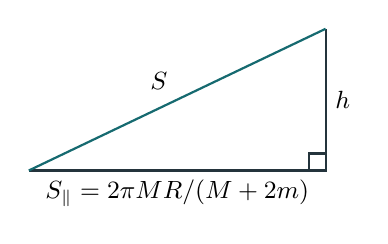
\begin{tikzpicture}[scale=1.8]
\draw[object] (0,0)--(2.0943951,0)--(2.0943951,1);
\draw[traj] (0,0)--(2.0943951,1);
\draw[object] (1.9743951,0)--(1.9743951,.12)--(2.0943951,.12);
\node[below] at (1.0471976,0) {$S_\parallel=2\pi MR/(M+2m)$};
\node[right] at (2.0943951,.5) {$h$};
\node[above left] at (1.0471976,.5) {$S$};
\end{tikzpicture}
\figcaption{解图力试1.3D\quad 地面螺旋展开后的水平弧长、下降量与总路程}
\end{minipage}\end{center}
地面水平长度包含两个因素：半径由$R$缩成$MR/(M+m)$，方位角由相对一周缩成$2\pi(M+m)/(M+2m)$。两者相乘才出现$M+2m$。当$M$很大时，筒轴半径趋零、反向自转趋零，球的路程趋向固定槽长$\sqrt{h^2+4\pi^2R^2}$；对任意有限正质量，地面水平弧长较小，重力只改变通过这条固定几何轨迹的快慢。


\Needspace{13\baselineskip}

\pdfbookmark[2]{第 4 题 弹出小球与自由细杆端点再次相遇}{q4}

\section*{第 4 题\quad 弹出小球与自由细杆端点再次相遇}\label{q:4}


质量为$M$、长度为$l$的均匀细杆$AB$静止在光滑水平面上。$B$端的轻弹簧将质量为$m$的小球斜向弹出，弹出后小球的地面速度大小为$v$，与从$B$指向$A$的方向夹角为$\varphi$，$0<\varphi<\pi/2$。

要求小球自由运动后恰与杆的$A$端相遇，且相遇前细杆的转角不超过$\pi$。求质量比$\gamma=M/m$与发射角$\varphi$的关系及其允许范围。忽略球与杆的厚度、摩擦和弹簧质量，弹出后到再次相遇前球与杆无相互作用。


\begin{center}\begin{minipage}{.98\linewidth}\centering
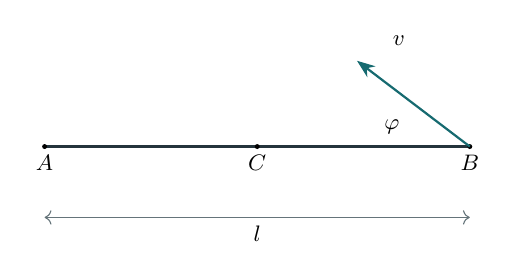
\begin{tikzpicture}[scale=.9,transform shape]
\draw[object] (-3.00000,0.00000)--(3.00000,0.00000);\fill (-3.00000,0.00000) circle(.035);\node[below] at (-3.00000,0.00000) {$A$};\fill (0.00000,0.00000) circle(.035);\node[below] at (0.00000,0.00000) {$C$};\fill (3.00000,0.00000) circle(.035);\node[below] at (3.00000,0.00000) {$B$};\draw[motion] (3.00000,0.00000)--(1.40783,1.21037);\node[above] at (2.00000,1.30000) {$v$};\node[above] at (1.90000,0.05000) {$\varphi$};\draw[<->,thin,color=muted] (-3.00000,-1.00000)--(3.00000,-1.00000);\node[below] at (0.00000,-1.00000) {$l$};
\end{tikzpicture}
\figcaption{图力试1.4\quad 斜向发射后，球和杆质心沿相反方向平移。}
\end{minipage}\end{center}

\Needspace{6\baselineskip}\subsection*{解答}


图力试1.4中，取初始杆质心$C$为坐标原点，$B=(l/2,0)$，$A=(-l/2,0)$。记$\gamma=M/m$。小球初速度为
\[
\boldsymbol v=v(-\cos\varphi,\sin\varphi).
\]
对冲量过程用水平动量守恒，细杆质心速度为
\[
\boldsymbol V_C=\frac{v}{\gamma}(\cos\varphi,-\sin\varphi).
\]
对细杆自身质心列转动冲量方程，端点$B$所受冲量与小球获得的冲量相反。杆的转动惯量$I_C=Ml^2/12$，故杆向顺时针转动，角速率
\[
I_C\Omega=\frac l2\,mv\sin\varphi,\qquad
\boxed{\Omega=\frac{6v\sin\varphi}{\gamma l}}.
\]
弹出后杆无水平力和竖直轴力矩，$\boldsymbol V_C,\Omega$均保持不变。

\begin{center}\begin{minipage}{.98\linewidth}\centering
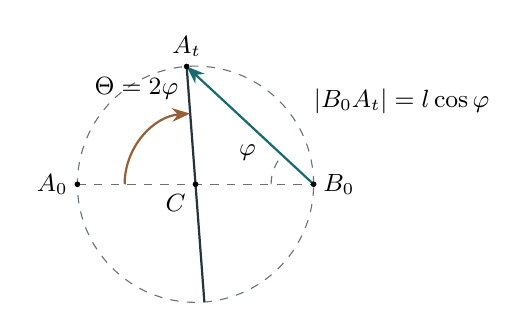
\begin{tikzpicture}[scale=3]
\draw[guide] (0,0) circle(.5);\draw[guide] (-.5,0)--(.5,0);
\draw[object] (-0.0374722,0.4985939)--(0.0374722,-0.4985939);
\draw[motion] (.5,0)--(-0.0374722,0.4985939);
\fill (.5,0) circle(.012) node[right] {$B_0$};\fill (-.5,0) circle(.012) node[left] {$A_0$};\fill (0,0) circle(.012) node[below left] {$C$};
\fill (-0.0374722,0.4985939) circle(.012) node[above] {$A_t$};
\draw[force] (-.3,0) arc(180:94.2980291:.3);
\draw[guide] (.32,0) arc(180:137.1490145:.18);
\node[above] at (-.25,.32) {$\Theta=2\varphi$};\node[above] at (.22,.06) {$\varphi$};
\node[right] at (.46,.35) {$|B_0A_t|=l\cos\varphi$};
\end{tikzpicture}
\figcaption{解图力试1.4A\quad 随C匀速平移的惯性系，球走弦而A端走短弧}
\end{minipage}\end{center}
解图力试1.4A在随$C$匀速平移、但坐标轴不转动的参考系中画图。小球相对速度是
\[
\boldsymbol w=\boldsymbol v-\boldsymbol V_C
=\left(1+\frac1\gamma\right)v(-\cos\varphi,\sin\varphi).
\]
于是小球从$B$沿直线行进，杆的$A$端沿半径$l/2$的圆周运动。设杆转过顺时针角$\Theta=\Omega t$。要求两者相遇，就要让该直线的第二个圆周交点恰好是此时的$A$端。

解图力试1.4A把弦$BA_t$与直径$BA$的夹角标为$\varphi$。相遇时
\[
A_t=\left(-\frac l2\cos\Theta,\frac l2\sin\Theta\right),
\qquad
A_t-B=\frac l2(-1-\cos\Theta,\sin\Theta).
\]
由两分量的比值，
\[
\tan\varphi=\frac{\sin\Theta}{1+\cos\Theta}
=\tan\frac{\Theta}{2}.
\]
在$0<\Theta\le\pi$的短弧分支中得到
\[
\Theta=2\varphi,\qquad |BA_t|=l\cos\varphi.
\]
弦长除以相对速率给相遇时间，故
\[
t=\frac{l\cos\varphi}{(1+1/\gamma)v},
\qquad
\Omega t=\frac{3\sin2\varphi}{1+\gamma}=2\varphi.
\]
因此所求配对关系是
\[
\boxed{\frac{1+\gamma}{3}=\frac{\sin2\varphi}{2\varphi}},
\qquad
\gamma=3\frac{\sin2\varphi}{2\varphi}-1.
\]
相遇条件只含质量比和几何角；提高发射速度会同时缩短球的飞行时间、加快杆的转动，两项在转角中抵消。

\begin{center}\begin{minipage}{.98\linewidth}\centering
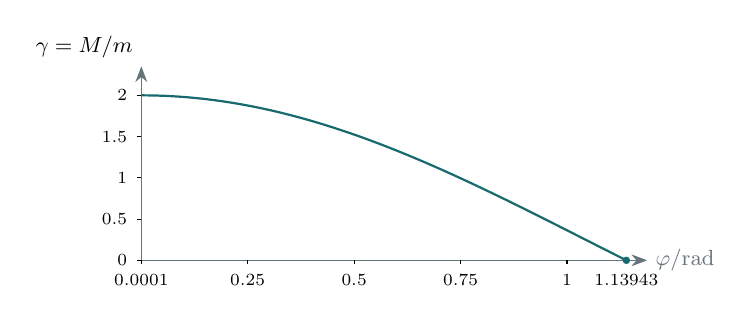
\begin{tikzpicture}[scale=.88,transform shape]
\draw[axis] (0,0.0)--(7.3,0.0) node[right] {$\varphi/\mathrm{rad}$};
\draw[axis] (0,0)--(0,2.8);
\node[above left] at (0,2.8) {$\gamma=M/m$};
\draw[thin] (0.000000,0.0)--(0.000000,-0.06);\node[below,font=\scriptsize] at (0.000000,-0.08) {$ 0.0001 $};
\draw[thin] (1.535374,0.0)--(1.535374,-0.06);\node[below,font=\scriptsize] at (1.535374,-0.08) {$ 0.25 $};
\draw[thin] (3.071363,0.0)--(3.071363,-0.06);\node[below,font=\scriptsize] at (3.071363,-0.08) {$ 0.5 $};
\draw[thin] (4.607352,0.0)--(4.607352,-0.06);\node[below,font=\scriptsize] at (4.607352,-0.08) {$ 0.75 $};
\draw[thin] (6.143340,0.0)--(6.143340,-0.06);\node[below,font=\scriptsize] at (6.143340,-0.08) {$ 1 $};
\draw[thin] (7.000000,0.0)--(7.000000,-0.06);\node[below,font=\scriptsize] at (7.000000,-0.08) {$ 1.13943 $};
\draw[thin] (0,0.000000)--(-.06,0.000000);\node[left,font=\scriptsize] at (-.08,0.000000) {$ 0 $};
\draw[thin] (0,0.595238)--(-.06,0.595238);\node[left,font=\scriptsize] at (-.08,0.595238) {$ 0.5 $};
\draw[thin] (0,1.190476)--(-.06,1.190476);\node[left,font=\scriptsize] at (-.08,1.190476) {$ 1 $};
\draw[thin] (0,1.785714)--(-.06,1.785714);\node[left,font=\scriptsize] at (-.08,1.785714) {$ 1.5 $};
\draw[thin] (0,2.380952)--(-.06,2.380952);\node[left,font=\scriptsize] at (-.08,2.380952) {$ 2 $};
\draw[thick,color=accent] plot coordinates {(0.0000000,2.3809524) (0.0291667,2.3808964) (0.0583333,2.3807332) (0.0875000,2.3804627) (0.1166667,2.3800849) (0.1458333,2.3795998) (0.1750000,2.3790075) (0.2041667,2.3783079) (0.2333333,2.3775012) (0.2625000,2.3765874) (0.2916667,2.3755665) (0.3208333,2.3744385) (0.3500000,2.3732036) (0.3791667,2.3718618) (0.4083333,2.3704132) (0.4375000,2.3688579) (0.4666667,2.3671959) (0.4958333,2.3654273) (0.5250000,2.3635522) (0.5541667,2.3615708) (0.5833333,2.3594831) (0.6125000,2.3572892) (0.6416667,2.3549893) (0.6708333,2.3525835) (0.7000000,2.3500720) (0.7291667,2.3474547) (0.7583333,2.3447320) (0.7875000,2.3419039) (0.8166667,2.3389706) (0.8458333,2.3359323) (0.8750000,2.3327891) (0.9041667,2.3295412) (0.9333333,2.3261887) (0.9625000,2.3227319) (0.9916667,2.3191709) (1.0208333,2.3155060) (1.0500000,2.3117372) (1.0791667,2.3078649) (1.1083333,2.3038892) (1.1375000,2.2998104) (1.1666667,2.2956287) (1.1958333,2.2913442) (1.2250000,2.2869573) (1.2541667,2.2824681) (1.2833333,2.2778769) (1.3125000,2.2731840) (1.3416667,2.2683896) (1.3708333,2.2634939) (1.4000000,2.2584973) (1.4291667,2.2534000) (1.4583333,2.2482022) (1.4875000,2.2429043) (1.5166667,2.2375065) (1.5458333,2.2320092) (1.5750000,2.2264126) (1.6041667,2.2207170) (1.6333333,2.2149227) (1.6625000,2.2090301) (1.6916667,2.2030394) (1.7208333,2.1969510) (1.7500000,2.1907652) (1.7791667,2.1844824) (1.8083333,2.1781028) (1.8375000,2.1716269) (1.8666667,2.1650549) (1.8958333,2.1583872) (1.9250000,2.1516243) (1.9541667,2.1447663) (1.9833333,2.1378138) (2.0125000,2.1307671) (2.0416667,2.1236265) (2.0708333,2.1163925) (2.1000000,2.1090654) (2.1291667,2.1016456) (2.1583333,2.0941336) (2.1875000,2.0865297) (2.2166667,2.0788343) (2.2458333,2.0710478) (2.2750000,2.0631708) (2.3041667,2.0552035) (2.3333333,2.0471464) (2.3625000,2.0389999) (2.3916667,2.0307646) (2.4208333,2.0224407) (2.4500000,2.0140288) (2.4791667,2.0055293) (2.5083333,1.9969427) (2.5375000,1.9882694) (2.5666667,1.9795099) (2.5958333,1.9706646) (2.6250000,1.9617341) (2.6541667,1.9527188) (2.6833333,1.9436191) (2.7125000,1.9344356) (2.7416667,1.9251688) (2.7708333,1.9158191) (2.8000000,1.9063871) (2.8291667,1.8968732) (2.8583333,1.8872779) (2.8875000,1.8776019) (2.9166667,1.8678455) (2.9458333,1.8580093) (2.9750000,1.8480938) (3.0041667,1.8380996) (3.0333333,1.8280271) (3.0625000,1.8178770) (3.0916667,1.8076497) (3.1208333,1.7973458) (3.1500000,1.7869658) (3.1791667,1.7765103) (3.2083333,1.7659799) (3.2375000,1.7553750) (3.2666667,1.7446963) (3.2958333,1.7339444) (3.3250000,1.7231197) (3.3541667,1.7122229) (3.3833333,1.7012545) (3.4125000,1.6902152) (3.4416667,1.6791054) (3.4708333,1.6679258) (3.5000000,1.6566770) (3.5291667,1.6453596) (3.5583333,1.6339741) (3.5875000,1.6225212) (3.6166667,1.6110015) (3.6458333,1.5994155) (3.6750000,1.5877639) (3.7041667,1.5760473) (3.7333333,1.5642663) (3.7625000,1.5524215) (3.7916667,1.5405136) (3.8208333,1.5285431) (3.8500000,1.5165108) (3.8791667,1.5044171) (3.9083333,1.4922628) (3.9375000,1.4800486) (3.9666667,1.4677749) (3.9958333,1.4554425) (4.0250000,1.4430521) (4.0541667,1.4306042) (4.0833333,1.4180995) (4.1125000,1.4055387) (4.1416667,1.3929224) (4.1708333,1.3802513) (4.2000000,1.3675260) (4.2291667,1.3547472) (4.2583333,1.3419156) (4.2875000,1.3290318) (4.3166667,1.3160965) (4.3458333,1.3031104) (4.3750000,1.2900741) (4.4041667,1.2769884) (4.4333333,1.2638538) (4.4625000,1.2506711) (4.4916667,1.2374410) (4.5208333,1.2241641) (4.5500000,1.2108411) (4.5791667,1.1974727) (4.6083333,1.1840597) (4.6375000,1.1706026) (4.6666667,1.1571022) (4.6958333,1.1435592) (4.7250000,1.1299743) (4.7541667,1.1163481) (4.7833333,1.1026815) (4.8125000,1.0889749) (4.8416667,1.0752293) (4.8708333,1.0614453) (4.9000000,1.0476235) (4.9291667,1.0337648) (4.9583333,1.0198697) (4.9875000,1.0059390) (5.0166667,0.9919735) (5.0458333,0.9779738) (5.0750000,0.9639407) (5.1041667,0.9498748) (5.1333333,0.9357769) (5.1625000,0.9216477) (5.1916667,0.9074879) (5.2208333,0.8932982) (5.2500000,0.8790794) (5.2791667,0.8648322) (5.3083333,0.8505572) (5.3375000,0.8362553) (5.3666667,0.8219271) (5.3958333,0.8075733) (5.4250000,0.7931947) (5.4541667,0.7787921) (5.4833333,0.7643660) (5.5125000,0.7499173) (5.5416667,0.7354467) (5.5708333,0.7209550) (5.6000000,0.7064427) (5.6291667,0.6919107) (5.6583333,0.6773597) (5.6875000,0.6627904) (5.7166667,0.6482035) (5.7458333,0.6335999) (5.7750000,0.6189801) (5.8041667,0.6043449) (5.8333333,0.5896951) (5.8625000,0.5750314) (5.8916667,0.5603545) (5.9208333,0.5456651) (5.9500000,0.5309640) (5.9791667,0.5162519) (6.0083333,0.5015294) (6.0375000,0.4867975) (6.0666667,0.4720567) (6.0958333,0.4573078) (6.1250000,0.4425515) (6.1541667,0.4277886) (6.1833333,0.4130198) (6.2125000,0.3982457) (6.2416667,0.3834671) (6.2708333,0.3686848) (6.3000000,0.3538995) (6.3291667,0.3391119) (6.3583333,0.3243226) (6.3875000,0.3095325) (6.4166667,0.2947422) (6.4458333,0.2799525) (6.4750000,0.2651640) (6.5041667,0.2503775) (6.5333333,0.2355938) (6.5625000,0.2208134) (6.5916667,0.2060372) (6.6208333,0.1912659) (6.6500000,0.1765001) (6.6791667,0.1617405) (6.7083333,0.1469879) (6.7375000,0.1322430) (6.7666667,0.1175065) (6.7958333,0.1027791) (6.8250000,0.0880614) (6.8541667,0.0733542) (6.8833333,0.0586582) (6.9125000,0.0439741) (6.9416667,0.0293026) (6.9708333,0.0146443) (7.0000000,-0.0000000)};
\draw[fill=white,color=accent] (7.0000000,-0.0000000) circle(.045);
\end{tikzpicture}
\figcaption{解图力试1.4B\quad 质量比与发射角的唯一配对，两个极限端点均不取}
\end{minipage}\end{center}
解图力试1.4B画出质量比随发射角的变化。为判断允许范围，令$x=2\varphi\in(0,\pi)$。函数$f(x)=\sin x/x$严格下降，因为
\[
f'(x)=\frac{x\cos x-\sin x}{x^2}<0;
\quad
\frac{\dd}{\dd x}(\sin x-x\cos x)=x\sin x>0.
\]
它从1降到0。再结合$\gamma>0$，得到
\[
\boxed{0<\gamma<2,\qquad 0<\varphi<\varphi_0},
\quad
\frac{\sin2\varphi_0}{2\varphi_0}=\frac13,
\quad \varphi_0\simeq1.1394\,\mathrm{rad}.
\]
对任意给定$0<\gamma<2$，有且只有一个允许发射角；质量比与角度通过上式一一配对，两个范围共同受同一等式约束。

同一相遇解还给出碰撞前球到杆身的法向距离。在$0<\Theta<2\varphi$时，小球位置为
\[
\boldsymbol r(\Theta)=\frac l2(1,0)
+\frac{l\Theta\cos\varphi}{2\varphi}
(-\cos\varphi,\sin\varphi).
\]
球到杆的有向直线的法向距离，乘$2/l$后为
\[
\frac{2}{l}\,\boldsymbol r(\Theta)\cdot
(\sin\Theta,\cos\Theta)
=\sin\Theta+
\frac{\Theta\cos\varphi}{\varphi}\sin(\varphi-\Theta)>0.
\]
在$0<\Theta\le\varphi$，两项均非负且第一项为正。在$\varphi<\Theta<2\varphi$，利用
\[
\frac{\sin\Theta}{\Theta}>
\frac{\sin2\varphi}{2\varphi}
=\frac{\cos\varphi\sin\varphi}{\varphi}
\ge\frac{\cos\varphi}{\varphi}\sin(\Theta-\varphi)
\]
也得严格正值。因此再次相交在$A_t$。解图力试1.4C画出相等质量时这段法向距离，开区间内为正，末端回到零。
\begin{center}\begin{minipage}{.98\linewidth}\centering
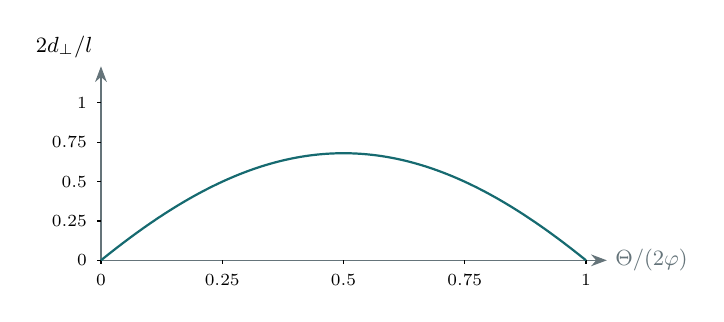
\begin{tikzpicture}[scale=.88,transform shape]
\draw[axis] (0,0.0)--(7.3,0.0) node[right] {$\Theta/(2\varphi)$};
\draw[axis] (0,0)--(0,2.8);
\node[above left] at (0,2.8) {$2d_\perp/l$};
\draw[thin] (0.000000,0.0)--(0.000000,-0.06);\node[below,font=\scriptsize] at (0.000000,-0.08) {$ 0 $};
\draw[thin] (1.750000,0.0)--(1.750000,-0.06);\node[below,font=\scriptsize] at (1.750000,-0.08) {$ 0.25 $};
\draw[thin] (3.500000,0.0)--(3.500000,-0.06);\node[below,font=\scriptsize] at (3.500000,-0.08) {$ 0.5 $};
\draw[thin] (5.250000,0.0)--(5.250000,-0.06);\node[below,font=\scriptsize] at (5.250000,-0.08) {$ 0.75 $};
\draw[thin] (7.000000,0.0)--(7.000000,-0.06);\node[below,font=\scriptsize] at (7.000000,-0.08) {$ 1 $};
\draw[thin] (0,0.000000)--(-.06,0.000000);\node[left,font=\scriptsize] at (-.08,0.000000) {$ 0 $};
\draw[thin] (0,0.568182)--(-.06,0.568182);\node[left,font=\scriptsize] at (-.08,0.568182) {$ 0.25 $};
\draw[thin] (0,1.136364)--(-.06,1.136364);\node[left,font=\scriptsize] at (-.08,1.136364) {$ 0.5 $};
\draw[thin] (0,1.704545)--(-.06,1.704545);\node[left,font=\scriptsize] at (-.08,1.704545) {$ 0.75 $};
\draw[thin] (0,2.272727)--(-.06,2.272727);\node[left,font=\scriptsize] at (-.08,2.272727) {$ 1 $};
\draw[thick,color=accent] plot coordinates {(0.0000000,0.0000000) (0.0291667,0.0235439) (0.0583333,0.0469594) (0.0875000,0.0702446) (0.1166667,0.0933981) (0.1458333,0.1164181) (0.1750000,0.1393032) (0.2041667,0.1620516) (0.2333333,0.1846619) (0.2625000,0.2071323) (0.2916667,0.2294615) (0.3208333,0.2516478) (0.3500000,0.2736896) (0.3791667,0.2955855) (0.4083333,0.3173339) (0.4375000,0.3389333) (0.4666667,0.3603823) (0.4958333,0.3816793) (0.5250000,0.4028228) (0.5541667,0.4238114) (0.5833333,0.4446437) (0.6125000,0.4653181) (0.6416667,0.4858334) (0.6708333,0.5061879) (0.7000000,0.5263804) (0.7291667,0.5464095) (0.7583333,0.5662737) (0.7875000,0.5859717) (0.8166667,0.6055022) (0.8458333,0.6248637) (0.8750000,0.6440550) (0.9041667,0.6630747) (0.9333333,0.6819216) (0.9625000,0.7005942) (0.9916667,0.7190914) (1.0208333,0.7374119) (1.0500000,0.7555544) (1.0791667,0.7735176) (1.1083333,0.7913004) (1.1375000,0.8089014) (1.1666667,0.8263196) (1.1958333,0.8435536) (1.2250000,0.8606024) (1.2541667,0.8774648) (1.2833333,0.8941395) (1.3125000,0.9106255) (1.3416667,0.9269216) (1.3708333,0.9430267) (1.4000000,0.9589397) (1.4291667,0.9746595) (1.4583333,0.9901851) (1.4875000,1.0055153) (1.5166667,1.0206492) (1.5458333,1.0355856) (1.5750000,1.0503237) (1.6041667,1.0648623) (1.6333333,1.0792004) (1.6625000,1.0933372) (1.6916667,1.1072716) (1.7208333,1.1210027) (1.7500000,1.1345295) (1.7791667,1.1478511) (1.8083333,1.1609667) (1.8375000,1.1738753) (1.8666667,1.1865760) (1.8958333,1.1990679) (1.9250000,1.2113503) (1.9541667,1.2234223) (1.9833333,1.2352831) (2.0125000,1.2469318) (2.0416667,1.2583676) (2.0708333,1.2695899) (2.1000000,1.2805977) (2.1291667,1.2913905) (2.1583333,1.3019673) (2.1875000,1.3123276) (2.2166667,1.3224706) (2.2458333,1.3323957) (2.2750000,1.3421021) (2.3041667,1.3515892) (2.3333333,1.3608563) (2.3625000,1.3699028) (2.3916667,1.3787282) (2.4208333,1.3873317) (2.4500000,1.3957129) (2.4791667,1.4038711) (2.5083333,1.4118058) (2.5375000,1.4195165) (2.5666667,1.4270027) (2.5958333,1.4342637) (2.6250000,1.4412992) (2.6541667,1.4481086) (2.6833333,1.4546916) (2.7125000,1.4610476) (2.7416667,1.4671762) (2.7708333,1.4730770) (2.8000000,1.4787496) (2.8291667,1.4841937) (2.8583333,1.4894088) (2.8875000,1.4943946) (2.9166667,1.4991507) (2.9458333,1.5036769) (2.9750000,1.5079729) (3.0041667,1.5120382) (3.0333333,1.5158728) (3.0625000,1.5194762) (3.0916667,1.5228483) (3.1208333,1.5259889) (3.1500000,1.5288976) (3.1791667,1.5315744) (3.2083333,1.5340190) (3.2375000,1.5362313) (3.2666667,1.5382112) (3.2958333,1.5399584) (3.3250000,1.5414729) (3.3541667,1.5427546) (3.3833333,1.5438034) (3.4125000,1.5446191) (3.4416667,1.5452019) (3.4708333,1.5455515) (3.5000000,1.5456681) (3.5291667,1.5455515) (3.5583333,1.5452019) (3.5875000,1.5446191) (3.6166667,1.5438034) (3.6458333,1.5427546) (3.6750000,1.5414729) (3.7041667,1.5399584) (3.7333333,1.5382112) (3.7625000,1.5362313) (3.7916667,1.5340190) (3.8208333,1.5315744) (3.8500000,1.5288976) (3.8791667,1.5259889) (3.9083333,1.5228483) (3.9375000,1.5194762) (3.9666667,1.5158728) (3.9958333,1.5120382) (4.0250000,1.5079729) (4.0541667,1.5036769) (4.0833333,1.4991507) (4.1125000,1.4943946) (4.1416667,1.4894088) (4.1708333,1.4841937) (4.2000000,1.4787496) (4.2291667,1.4730770) (4.2583333,1.4671762) (4.2875000,1.4610476) (4.3166667,1.4546916) (4.3458333,1.4481086) (4.3750000,1.4412992) (4.4041667,1.4342637) (4.4333333,1.4270027) (4.4625000,1.4195165) (4.4916667,1.4118058) (4.5208333,1.4038711) (4.5500000,1.3957129) (4.5791667,1.3873317) (4.6083333,1.3787282) (4.6375000,1.3699028) (4.6666667,1.3608563) (4.6958333,1.3515892) (4.7250000,1.3421021) (4.7541667,1.3323957) (4.7833333,1.3224706) (4.8125000,1.3123276) (4.8416667,1.3019673) (4.8708333,1.2913905) (4.9000000,1.2805977) (4.9291667,1.2695899) (4.9583333,1.2583676) (4.9875000,1.2469318) (5.0166667,1.2352831) (5.0458333,1.2234223) (5.0750000,1.2113503) (5.1041667,1.1990679) (5.1333333,1.1865760) (5.1625000,1.1738753) (5.1916667,1.1609667) (5.2208333,1.1478511) (5.2500000,1.1345295) (5.2791667,1.1210027) (5.3083333,1.1072716) (5.3375000,1.0933372) (5.3666667,1.0792004) (5.3958333,1.0648623) (5.4250000,1.0503237) (5.4541667,1.0355856) (5.4833333,1.0206492) (5.5125000,1.0055153) (5.5416667,0.9901851) (5.5708333,0.9746595) (5.6000000,0.9589397) (5.6291667,0.9430267) (5.6583333,0.9269216) (5.6875000,0.9106255) (5.7166667,0.8941395) (5.7458333,0.8774648) (5.7750000,0.8606024) (5.8041667,0.8435536) (5.8333333,0.8263196) (5.8625000,0.8089014) (5.8916667,0.7913004) (5.9208333,0.7735176) (5.9500000,0.7555544) (5.9791667,0.7374119) (6.0083333,0.7190914) (6.0375000,0.7005942) (6.0666667,0.6819216) (6.0958333,0.6630747) (6.1250000,0.6440550) (6.1541667,0.6248637) (6.1833333,0.6055022) (6.2125000,0.5859717) (6.2416667,0.5662737) (6.2708333,0.5464095) (6.3000000,0.5263804) (6.3291667,0.5061879) (6.3583333,0.4858334) (6.3875000,0.4653181) (6.4166667,0.4446437) (6.4458333,0.4238114) (6.4750000,0.4028228) (6.5041667,0.3816793) (6.5333333,0.3603823) (6.5625000,0.3389333) (6.5916667,0.3173339) (6.6208333,0.2955855) (6.6500000,0.2736896) (6.6791667,0.2516478) (6.7083333,0.2294615) (6.7375000,0.2071323) (6.7666667,0.1846619) (6.7958333,0.1620516) (6.8250000,0.1393032) (6.8541667,0.1164181) (6.8833333,0.0933981) (6.9125000,0.0702446) (6.9416667,0.0469594) (6.9708333,0.0235439) (7.0000000,-0.0000000)};
\end{tikzpicture}
\figcaption{解图力试1.4C\quad 相等质量时球到杆直线的有向法向距离}
\end{minipage}\end{center}
解图力试1.4D将同一相遇放回地面系，球走直线，杆质心沿反方向走直线，A端同时绕质心转动；两条地面轨迹在相遇时刻汇合。
\begin{center}\begin{minipage}{.98\linewidth}\centering
\begin{tikzpicture}[scale=4]
\draw[axis] (-.6,0)--(.7,0) node[right] {$x/l$};\draw[axis] (0,-.8)--(0,.45) node[above] {$y/l$};
\draw[thick,color=accent] plot coordinates {(0.5000000,0.0000000) (0.4988803,0.0010387) (0.4977605,0.0020775) (0.4966408,0.0031162) (0.4955211,0.0041549) (0.4944013,0.0051937) (0.4932816,0.0062324) (0.4921619,0.0072712) (0.4910421,0.0083099) (0.4899224,0.0093486) (0.4888027,0.0103874) (0.4876829,0.0114261) (0.4865632,0.0124648) (0.4854435,0.0135036) (0.4843237,0.0145423) (0.4832040,0.0155811) (0.4820843,0.0166198) (0.4809645,0.0176585) (0.4798448,0.0186973) (0.4787251,0.0197360) (0.4776053,0.0207747) (0.4764856,0.0218135) (0.4753659,0.0228522) (0.4742461,0.0238910) (0.4731264,0.0249297) (0.4720067,0.0259684) (0.4708869,0.0270072) (0.4697672,0.0280459) (0.4686475,0.0290846) (0.4675277,0.0301234) (0.4664080,0.0311621) (0.4652883,0.0322009) (0.4641685,0.0332396) (0.4630488,0.0342783) (0.4619291,0.0353171) (0.4608093,0.0363558) (0.4596896,0.0373945) (0.4585699,0.0384333) (0.4574501,0.0394720) (0.4563304,0.0405108) (0.4552106,0.0415495) (0.4540909,0.0425882) (0.4529712,0.0436270) (0.4518514,0.0446657) (0.4507317,0.0457044) (0.4496120,0.0467432) (0.4484922,0.0477819) (0.4473725,0.0488206) (0.4462528,0.0498594) (0.4451330,0.0508981) (0.4440133,0.0519369) (0.4428936,0.0529756) (0.4417738,0.0540143) (0.4406541,0.0550531) (0.4395344,0.0560918) (0.4384146,0.0571305) (0.4372949,0.0581693) (0.4361752,0.0592080) (0.4350554,0.0602468) (0.4339357,0.0612855) (0.4328160,0.0623242) (0.4316962,0.0633630) (0.4305765,0.0644017) (0.4294568,0.0654404) (0.4283370,0.0664792) (0.4272173,0.0675179) (0.4260976,0.0685567) (0.4249778,0.0695954) (0.4238581,0.0706341) (0.4227384,0.0716729) (0.4216186,0.0727116) (0.4204989,0.0737503) (0.4193792,0.0747891) (0.4182594,0.0758278) (0.4171397,0.0768666) (0.4160200,0.0779053) (0.4149002,0.0789440) (0.4137805,0.0799828) (0.4126608,0.0810215) (0.4115410,0.0820602) (0.4104213,0.0830990) (0.4093016,0.0841377) (0.4081818,0.0851765) (0.4070621,0.0862152) (0.4059424,0.0872539) (0.4048226,0.0882927) (0.4037029,0.0893314) (0.4025832,0.0903701) (0.4014634,0.0914089) (0.4003437,0.0924476) (0.3992240,0.0934863) (0.3981042,0.0945251) (0.3969845,0.0955638) (0.3958648,0.0966026) (0.3947450,0.0976413) (0.3936253,0.0986800) (0.3925056,0.0997188) (0.3913858,0.1007575) (0.3902661,0.1017962) (0.3891464,0.1028350) (0.3880266,0.1038737) (0.3869069,0.1049125) (0.3857872,0.1059512) (0.3846674,0.1069899) (0.3835477,0.1080287) (0.3824280,0.1090674) (0.3813082,0.1101061) (0.3801885,0.1111449) (0.3790688,0.1121836) (0.3779490,0.1132224) (0.3768293,0.1142611) (0.3757096,0.1152998) (0.3745898,0.1163386) (0.3734701,0.1173773) (0.3723503,0.1184160) (0.3712306,0.1194548) (0.3701109,0.1204935) (0.3689911,0.1215323) (0.3678714,0.1225710) (0.3667517,0.1236097) (0.3656319,0.1246485) (0.3645122,0.1256872) (0.3633925,0.1267259) (0.3622727,0.1277647) (0.3611530,0.1288034) (0.3600333,0.1298422) (0.3589135,0.1308809) (0.3577938,0.1319196) (0.3566741,0.1329584) (0.3555543,0.1339971) (0.3544346,0.1350358) (0.3533149,0.1360746) (0.3521951,0.1371133) (0.3510754,0.1381520) (0.3499557,0.1391908) (0.3488359,0.1402295) (0.3477162,0.1412683) (0.3465965,0.1423070) (0.3454767,0.1433457) (0.3443570,0.1443845) (0.3432373,0.1454232) (0.3421175,0.1464619) (0.3409978,0.1475007) (0.3398781,0.1485394) (0.3387583,0.1495782) (0.3376386,0.1506169) (0.3365189,0.1516556) (0.3353991,0.1526944) (0.3342794,0.1537331) (0.3331597,0.1547718) (0.3320399,0.1558106) (0.3309202,0.1568493) (0.3298005,0.1578881) (0.3286807,0.1589268) (0.3275610,0.1599655) (0.3264413,0.1610043) (0.3253215,0.1620430) (0.3242018,0.1630817) (0.3230821,0.1641205) (0.3219623,0.1651592) (0.3208426,0.1661980) (0.3197229,0.1672367) (0.3186031,0.1682754) (0.3174834,0.1693142) (0.3163637,0.1703529) (0.3152439,0.1713916) (0.3141242,0.1724304) (0.3130045,0.1734691) (0.3118847,0.1745078) (0.3107650,0.1755466) (0.3096453,0.1765853) (0.3085255,0.1776241) (0.3074058,0.1786628) (0.3062861,0.1797015) (0.3051663,0.1807403) (0.3040466,0.1817790) (0.3029269,0.1828177) (0.3018071,0.1838565) (0.3006874,0.1848952) (0.2995677,0.1859340) (0.2984479,0.1869727) (0.2973282,0.1880114) (0.2962085,0.1890502) (0.2950887,0.1900889) (0.2939690,0.1911276) (0.2928493,0.1921664) (0.2917295,0.1932051) (0.2906098,0.1942439) (0.2894901,0.1952826) (0.2883703,0.1963213) (0.2872506,0.1973601) (0.2861308,0.1983988) (0.2850111,0.1994375) (0.2838914,0.2004763) (0.2827716,0.2015150) (0.2816519,0.2025538) (0.2805322,0.2035925) (0.2794124,0.2046312) (0.2782927,0.2056700) (0.2771730,0.2067087) (0.2760532,0.2077474) (0.2749335,0.2087862) (0.2738138,0.2098249) (0.2726940,0.2108637) (0.2715743,0.2119024) (0.2704546,0.2129411) (0.2693348,0.2139799) (0.2682151,0.2150186) (0.2670954,0.2160573) (0.2659756,0.2170961) (0.2648559,0.2181348) (0.2637362,0.2191735) (0.2626164,0.2202123) (0.2614967,0.2212510) (0.2603770,0.2222898) (0.2592572,0.2233285) (0.2581375,0.2243672) (0.2570178,0.2254060) (0.2558980,0.2264447) (0.2547783,0.2274834) (0.2536586,0.2285222) (0.2525388,0.2295609) (0.2514191,0.2305997) (0.2502994,0.2316384) (0.2491796,0.2326771) (0.2480599,0.2337159) (0.2469402,0.2347546) (0.2458204,0.2357933) (0.2447007,0.2368321) (0.2435810,0.2378708) (0.2424612,0.2389096) (0.2413415,0.2399483) (0.2402218,0.2409870) (0.2391020,0.2420258) (0.2379823,0.2430645) (0.2368626,0.2441032) (0.2357428,0.2451420) (0.2346231,0.2461807) (0.2335034,0.2472195) (0.2323836,0.2482582) (0.2312639,0.2492969)};
\draw[thick,dashed,color=warm] plot coordinates {(-0.5000000,0.0000000) (-0.4988706,0.0020775) (-0.4977217,0.0041548) (-0.4965534,0.0062319) (-0.4953657,0.0083086) (-0.4941586,0.0103849) (-0.4929321,0.0124605) (-0.4916861,0.0145354) (-0.4904208,0.0166095) (-0.4891360,0.0186826) (-0.4878319,0.0207546) (-0.4865084,0.0228254) (-0.4851655,0.0248948) (-0.4838032,0.0269629) (-0.4824216,0.0290293) (-0.4810207,0.0310941) (-0.4796004,0.0331570) (-0.4781607,0.0352180) (-0.4767018,0.0372770) (-0.4752236,0.0393337) (-0.4737260,0.0413882) (-0.4722092,0.0434403) (-0.4706732,0.0454898) (-0.4691179,0.0475367) (-0.4675434,0.0495808) (-0.4659497,0.0516220) (-0.4643368,0.0536602) (-0.4627047,0.0556953) (-0.4610535,0.0577271) (-0.4593832,0.0597555) (-0.4576937,0.0617805) (-0.4559852,0.0638018) (-0.4542576,0.0658194) (-0.4525110,0.0678332) (-0.4507453,0.0698430) (-0.4489607,0.0718487) (-0.4471571,0.0738502) (-0.4453346,0.0758474) (-0.4434932,0.0778401) (-0.4416329,0.0798283) (-0.4397537,0.0818119) (-0.4378557,0.0837906) (-0.4359390,0.0857644) (-0.4340034,0.0877332) (-0.4320492,0.0896968) (-0.4300762,0.0916552) (-0.4280846,0.0936082) (-0.4260744,0.0955558) (-0.4240455,0.0974977) (-0.4219981,0.0994339) (-0.4199322,0.1013642) (-0.4178478,0.1032886) (-0.4157449,0.1052069) (-0.4136237,0.1071191) (-0.4114840,0.1090249) (-0.4093261,0.1109243) (-0.4071498,0.1128172) (-0.4049553,0.1147035) (-0.4027426,0.1165830) (-0.4005117,0.1184556) (-0.3982627,0.1203213) (-0.3959956,0.1221798) (-0.3937104,0.1240312) (-0.3914073,0.1258752) (-0.3890863,0.1277118) (-0.3867473,0.1295409) (-0.3843905,0.1313623) (-0.3820159,0.1331759) (-0.3796236,0.1349817) (-0.3772135,0.1367794) (-0.3747858,0.1385691) (-0.3723405,0.1403506) (-0.3698776,0.1421237) (-0.3673972,0.1438885) (-0.3648994,0.1456447) (-0.3623842,0.1473922) (-0.3598517,0.1491310) (-0.3573018,0.1508610) (-0.3547348,0.1525819) (-0.3521506,0.1542938) (-0.3495492,0.1559966) (-0.3469308,0.1576900) (-0.3442954,0.1593740) (-0.3416431,0.1610486) (-0.3389739,0.1627135) (-0.3362878,0.1643687) (-0.3335850,0.1660141) (-0.3308655,0.1676496) (-0.3281294,0.1692751) (-0.3253767,0.1708904) (-0.3226075,0.1724956) (-0.3198218,0.1740904) (-0.3170198,0.1756747) (-0.3142014,0.1772485) (-0.3113668,0.1788117) (-0.3085161,0.1803641) (-0.3056492,0.1819057) (-0.3027662,0.1834364) (-0.2998673,0.1849560) (-0.2969524,0.1864645) (-0.2940218,0.1879618) (-0.2910753,0.1894477) (-0.2881132,0.1909221) (-0.2851354,0.1923851) (-0.2821421,0.1938364) (-0.2791332,0.1952760) (-0.2761090,0.1967038) (-0.2730695,0.1981196) (-0.2700146,0.1995235) (-0.2669446,0.2009152) (-0.2638595,0.2022947) (-0.2607594,0.2036620) (-0.2576443,0.2050168) (-0.2545143,0.2063592) (-0.2513695,0.2076890) (-0.2482100,0.2090061) (-0.2450359,0.2103105) (-0.2418471,0.2116020) (-0.2386439,0.2128805) (-0.2354263,0.2141461) (-0.2321944,0.2153985) (-0.2289483,0.2166377) (-0.2256880,0.2178636) (-0.2224136,0.2190762) (-0.2191252,0.2202752) (-0.2158229,0.2214607) (-0.2125068,0.2226326) (-0.2091770,0.2237907) (-0.2058335,0.2249350) (-0.2024765,0.2260654) (-0.1991060,0.2271819) (-0.1957220,0.2282842) (-0.1923248,0.2293724) (-0.1889144,0.2304464) (-0.1854909,0.2315060) (-0.1820543,0.2325513) (-0.1786048,0.2335820) (-0.1751424,0.2345983) (-0.1716673,0.2355998) (-0.1681795,0.2365867) (-0.1646791,0.2375587) (-0.1611662,0.2385159) (-0.1576410,0.2394581) (-0.1541034,0.2403853) (-0.1505536,0.2412974) (-0.1469918,0.2421943) (-0.1434179,0.2430759) (-0.1398321,0.2439422) (-0.1362344,0.2447931) (-0.1326251,0.2456286) (-0.1290041,0.2464484) (-0.1253715,0.2472527) (-0.1217276,0.2480412) (-0.1180723,0.2488140) (-0.1144057,0.2495709) (-0.1107280,0.2503120) (-0.1070393,0.2510370) (-0.1033396,0.2517460) (-0.0996291,0.2524389) (-0.0959078,0.2531157) (-0.0921759,0.2537761) (-0.0884335,0.2544203) (-0.0846806,0.2550481) (-0.0809174,0.2556594) (-0.0771439,0.2562542) (-0.0733603,0.2568325) (-0.0695667,0.2573941) (-0.0657632,0.2579391) (-0.0619499,0.2584672) (-0.0581268,0.2589786) (-0.0542941,0.2594731) (-0.0504520,0.2599506) (-0.0466004,0.2604111) (-0.0427396,0.2608546) (-0.0388695,0.2612810) (-0.0349904,0.2616902) (-0.0311023,0.2620822) (-0.0272054,0.2624569) (-0.0232997,0.2628143) (-0.0193853,0.2631542) (-0.0154624,0.2634768) (-0.0115311,0.2637818) (-0.0075914,0.2640693) (-0.0036436,0.2643392) (0.0003124,0.2645914) (0.0042763,0.2648259) (0.0082481,0.2650427) (0.0122277,0.2652417) (0.0162150,0.2654228) (0.0202098,0.2655860) (0.0242120,0.2657313) (0.0282216,0.2658586) (0.0322383,0.2659679) (0.0362622,0.2660591) (0.0402931,0.2661322) (0.0443308,0.2661871) (0.0483753,0.2662238) (0.0524264,0.2662422) (0.0564841,0.2662424) (0.0605482,0.2662242) (0.0646185,0.2661877) (0.0686951,0.2661328) (0.0727778,0.2660594) (0.0768664,0.2659675) (0.0809608,0.2658571) (0.0850610,0.2657281) (0.0891668,0.2655806) (0.0932781,0.2654144) (0.0973947,0.2652296) (0.1015167,0.2650260) (0.1056437,0.2648038) (0.1097759,0.2645627) (0.1139129,0.2643029) (0.1180547,0.2640243) (0.1222012,0.2637268) (0.1263522,0.2634105) (0.1305077,0.2630752) (0.1346676,0.2627210) (0.1388316,0.2623478) (0.1429997,0.2619557) (0.1471718,0.2615445) (0.1513477,0.2611143) (0.1555274,0.2606651) (0.1597107,0.2601968) (0.1638975,0.2597093) (0.1680877,0.2592028) (0.1722811,0.2586770) (0.1764776,0.2581322) (0.1806772,0.2575681) (0.1848797,0.2569848) (0.1890849,0.2563824) (0.1932929,0.2557606) (0.1975033,0.2551196) (0.2017162,0.2544594) (0.2059313,0.2537799) (0.2101487,0.2530810) (0.2143681,0.2523629) (0.2185894,0.2516254) (0.2228126,0.2508686) (0.2270375,0.2500924) (0.2312639,0.2492969)};
\draw[thin,densely dotted,color=muted] plot coordinates {(0.0000000,-0.0000000) (0.0011197,-0.0010387) (0.0022395,-0.0020775) (0.0033592,-0.0031162) (0.0044789,-0.0041549) (0.0055987,-0.0051937) (0.0067184,-0.0062324) (0.0078381,-0.0072712) (0.0089579,-0.0083099) (0.0100776,-0.0093486) (0.0111973,-0.0103874) (0.0123171,-0.0114261) (0.0134368,-0.0124648) (0.0145565,-0.0135036) (0.0156763,-0.0145423) (0.0167960,-0.0155811) (0.0179157,-0.0166198) (0.0190355,-0.0176585) (0.0201552,-0.0186973) (0.0212749,-0.0197360) (0.0223947,-0.0207747) (0.0235144,-0.0218135) (0.0246341,-0.0228522) (0.0257539,-0.0238910) (0.0268736,-0.0249297) (0.0279933,-0.0259684) (0.0291131,-0.0270072) (0.0302328,-0.0280459) (0.0313525,-0.0290846) (0.0324723,-0.0301234) (0.0335920,-0.0311621) (0.0347117,-0.0322009) (0.0358315,-0.0332396) (0.0369512,-0.0342783) (0.0380709,-0.0353171) (0.0391907,-0.0363558) (0.0403104,-0.0373945) (0.0414301,-0.0384333) (0.0425499,-0.0394720) (0.0436696,-0.0405108) (0.0447894,-0.0415495) (0.0459091,-0.0425882) (0.0470288,-0.0436270) (0.0481486,-0.0446657) (0.0492683,-0.0457044) (0.0503880,-0.0467432) (0.0515078,-0.0477819) (0.0526275,-0.0488206) (0.0537472,-0.0498594) (0.0548670,-0.0508981) (0.0559867,-0.0519369) (0.0571064,-0.0529756) (0.0582262,-0.0540143) (0.0593459,-0.0550531) (0.0604656,-0.0560918) (0.0615854,-0.0571305) (0.0627051,-0.0581693) (0.0638248,-0.0592080) (0.0649446,-0.0602468) (0.0660643,-0.0612855) (0.0671840,-0.0623242) (0.0683038,-0.0633630) (0.0694235,-0.0644017) (0.0705432,-0.0654404) (0.0716630,-0.0664792) (0.0727827,-0.0675179) (0.0739024,-0.0685567) (0.0750222,-0.0695954) (0.0761419,-0.0706341) (0.0772616,-0.0716729) (0.0783814,-0.0727116) (0.0795011,-0.0737503) (0.0806208,-0.0747891) (0.0817406,-0.0758278) (0.0828603,-0.0768666) (0.0839800,-0.0779053) (0.0850998,-0.0789440) (0.0862195,-0.0799828) (0.0873392,-0.0810215) (0.0884590,-0.0820602) (0.0895787,-0.0830990) (0.0906984,-0.0841377) (0.0918182,-0.0851765) (0.0929379,-0.0862152) (0.0940576,-0.0872539) (0.0951774,-0.0882927) (0.0962971,-0.0893314) (0.0974168,-0.0903701) (0.0985366,-0.0914089) (0.0996563,-0.0924476) (0.1007760,-0.0934863) (0.1018958,-0.0945251) (0.1030155,-0.0955638) (0.1041352,-0.0966026) (0.1052550,-0.0976413) (0.1063747,-0.0986800) (0.1074944,-0.0997188) (0.1086142,-0.1007575) (0.1097339,-0.1017962) (0.1108536,-0.1028350) (0.1119734,-0.1038737) (0.1130931,-0.1049125) (0.1142128,-0.1059512) (0.1153326,-0.1069899) (0.1164523,-0.1080287) (0.1175720,-0.1090674) (0.1186918,-0.1101061) (0.1198115,-0.1111449) (0.1209312,-0.1121836) (0.1220510,-0.1132224) (0.1231707,-0.1142611) (0.1242904,-0.1152998) (0.1254102,-0.1163386) (0.1265299,-0.1173773) (0.1276497,-0.1184160) (0.1287694,-0.1194548) (0.1298891,-0.1204935) (0.1310089,-0.1215323) (0.1321286,-0.1225710) (0.1332483,-0.1236097) (0.1343681,-0.1246485) (0.1354878,-0.1256872) (0.1366075,-0.1267259) (0.1377273,-0.1277647) (0.1388470,-0.1288034) (0.1399667,-0.1298422) (0.1410865,-0.1308809) (0.1422062,-0.1319196) (0.1433259,-0.1329584) (0.1444457,-0.1339971) (0.1455654,-0.1350358) (0.1466851,-0.1360746) (0.1478049,-0.1371133) (0.1489246,-0.1381520) (0.1500443,-0.1391908) (0.1511641,-0.1402295) (0.1522838,-0.1412683) (0.1534035,-0.1423070) (0.1545233,-0.1433457) (0.1556430,-0.1443845) (0.1567627,-0.1454232) (0.1578825,-0.1464619) (0.1590022,-0.1475007) (0.1601219,-0.1485394) (0.1612417,-0.1495782) (0.1623614,-0.1506169) (0.1634811,-0.1516556) (0.1646009,-0.1526944) (0.1657206,-0.1537331) (0.1668403,-0.1547718) (0.1679601,-0.1558106) (0.1690798,-0.1568493) (0.1701995,-0.1578881) (0.1713193,-0.1589268) (0.1724390,-0.1599655) (0.1735587,-0.1610043) (0.1746785,-0.1620430) (0.1757982,-0.1630817) (0.1769179,-0.1641205) (0.1780377,-0.1651592) (0.1791574,-0.1661980) (0.1802771,-0.1672367) (0.1813969,-0.1682754) (0.1825166,-0.1693142) (0.1836363,-0.1703529) (0.1847561,-0.1713916) (0.1858758,-0.1724304) (0.1869955,-0.1734691) (0.1881153,-0.1745078) (0.1892350,-0.1755466) (0.1903547,-0.1765853) (0.1914745,-0.1776241) (0.1925942,-0.1786628) (0.1937139,-0.1797015) (0.1948337,-0.1807403) (0.1959534,-0.1817790) (0.1970731,-0.1828177) (0.1981929,-0.1838565) (0.1993126,-0.1848952) (0.2004323,-0.1859340) (0.2015521,-0.1869727) (0.2026718,-0.1880114) (0.2037915,-0.1890502) (0.2049113,-0.1900889) (0.2060310,-0.1911276) (0.2071507,-0.1921664) (0.2082705,-0.1932051) (0.2093902,-0.1942439) (0.2105099,-0.1952826) (0.2116297,-0.1963213) (0.2127494,-0.1973601) (0.2138692,-0.1983988) (0.2149889,-0.1994375) (0.2161086,-0.2004763) (0.2172284,-0.2015150) (0.2183481,-0.2025538) (0.2194678,-0.2035925) (0.2205876,-0.2046312) (0.2217073,-0.2056700) (0.2228270,-0.2067087) (0.2239468,-0.2077474) (0.2250665,-0.2087862) (0.2261862,-0.2098249) (0.2273060,-0.2108637) (0.2284257,-0.2119024) (0.2295454,-0.2129411) (0.2306652,-0.2139799) (0.2317849,-0.2150186) (0.2329046,-0.2160573) (0.2340244,-0.2170961) (0.2351441,-0.2181348) (0.2362638,-0.2191735) (0.2373836,-0.2202123) (0.2385033,-0.2212510) (0.2396230,-0.2222898) (0.2407428,-0.2233285) (0.2418625,-0.2243672) (0.2429822,-0.2254060) (0.2441020,-0.2264447) (0.2452217,-0.2274834) (0.2463414,-0.2285222) (0.2474612,-0.2295609) (0.2485809,-0.2305997) (0.2497006,-0.2316384) (0.2508204,-0.2326771) (0.2519401,-0.2337159) (0.2530598,-0.2347546) (0.2541796,-0.2357933) (0.2552993,-0.2368321) (0.2564190,-0.2378708) (0.2575388,-0.2389096) (0.2586585,-0.2399483) (0.2597782,-0.2409870) (0.2608980,-0.2420258) (0.2620177,-0.2430645) (0.2631374,-0.2441032) (0.2642572,-0.2451420) (0.2653769,-0.2461807) (0.2664966,-0.2472195) (0.2676164,-0.2482582) (0.2687361,-0.2492969)};
\draw[thin,color=muted] (-0.5000000,0.0000000)--(0.5000000,-0.0000000);
\draw[thin,color=muted] (-0.2321944,0.2153985)--(0.5009305,-0.4646954);
\draw[thin,color=muted] (0.2312639,0.2492969)--(0.3062083,-0.7478908);
\fill (0.2312639,0.2492969) circle(.012) node[above right] {$Q$};
\node[right] at (.72,.32) {球：实线};\node[right] at (.72,.2) {A端：虚线};\node[right] at (.72,.08) {C：点线};
\end{tikzpicture}
\figcaption{解图力试1.4D\quad 相等质量的地面轨迹与杆的三个时刻位置}
\end{minipage}\end{center}

$\varphi=0$对应沿杆身前进的共线过程，题设斜向离杆的运动对应$\varphi>0$。当$\varphi\to0^+$时，$\gamma\to2^-$，两个端点以严格不等号作为该过程的极限。


\Needspace{13\baselineskip}

\pdfbookmark[2]{第 5 题 切向减速后的陨石近地点}{q5}

\section*{第 5 题\quad 切向减速后的陨石近地点}\label{q:5}


一块陨石在距地表高度$h=4.2\times10^3\,\mathrm{km}$的圆轨道上绕地球运动，突然与一块小得多的陨石正碰，碰后动能减少2\%。把碰撞视为瞬时过程，假定大陨石质量不变，运动方向不变，随后只受地球引力。

求碰撞后陨石离地心的最小距离。地球半径$R_E=6.4\times10^3\,\mathrm{km}$；引力按球对称处理，忽略大气阻力。


\begin{center}\begin{minipage}{.98\linewidth}\centering
\begin{tikzpicture}[scale=.9,transform shape]
\draw[object] (0,0) circle(1.8113208);
\node at (0,0) {地球};\draw[guide] (0,0) circle(3);
\fill (3,0) circle(.04) node[right] {$A$碰撞};\draw[motion] (3,0)--(3,1.4) node[right] {$v_0\to v_+$};
\draw[<->,thin,color=muted] (0,-2.4)--(3,-2.4) node[midway,below] {$r_0=R_E+h$};
\end{tikzpicture}
\figcaption{图力试1.5\quad 地球与圆轨道半径按题设比例绘制，碰撞点速度沿切线减小}
\end{minipage}\end{center}

\Needspace{6\baselineskip}\subsection*{解答}


图力试1.5中碰撞点记为$A$。圆轨道半径为
\[
r_0=R_E+h=1.06\times10^4\,\mathrm{km}.
\]
令$\mu=GM_E$。碰撞前$v_0^2=\mu/r_0$，碰撞后动能为此前的$0.98$倍，所以
\[
v_+^2=0.98\,\frac{\mu}{r_0},\qquad
v_+=\sqrt{0.98}\,v_0.
\]
动能损失2\%对应速率按平方根降低约1\%，当前速度平方比例为0.98。

\begin{center}\begin{minipage}{.98\linewidth}\centering
\begin{tikzpicture}[scale=2.5]
\draw[object] (0,0) circle(0.6037736);
\fill (0,0) circle(.012) node[above] {$O$};\node at (0,-.15) {地球};
\draw[traj] plot coordinates {(1.0000000,0.0000000) (0.9996640,0.0256585) (0.9986564,0.0512995) (0.9969778,0.0769053) (0.9946293,0.1024584) (0.9916126,0.1279413) (0.9879297,0.1533364) (0.9835832,0.1786265) (0.9785761,0.2037942) (0.9729117,0.2288222) (0.9665939,0.2536934) (0.9596272,0.2783907) (0.9520162,0.3028972) (0.9437662,0.3271962) (0.9348828,0.3512709) (0.9253721,0.3751048) (0.9152406,0.3986817) (0.9044954,0.4219853) (0.8931437,0.4449997) (0.8811932,0.4677091) (0.8686524,0.4900980) (0.8555296,0.5121510) (0.8418339,0.5338530) (0.8275747,0.5551892) (0.8127618,0.5761448) (0.7974052,0.5967056) (0.7815156,0.6168574) (0.7651039,0.6365864) (0.7481812,0.6558792) (0.7307592,0.6747224) (0.7128498,0.6931033) (0.6944653,0.7110091) (0.6756182,0.7284276) (0.6563216,0.7453469) (0.6365886,0.7617554) (0.6164328,0.7776418) (0.5958679,0.7929953) (0.5749081,0.8078052) (0.5535677,0.8220616) (0.5318613,0.8357545) (0.5098039,0.8488747) (0.4874105,0.8614131) (0.4646966,0.8733611) (0.4416775,0.8847105) (0.4183693,0.8954537) (0.3947877,0.9055831) (0.3709490,0.9150919) (0.3468695,0.9239735) (0.3225657,0.9322218) (0.2980543,0.9398313) (0.2733520,0.9467967) (0.2484758,0.9531132) (0.2234428,0.9587764) (0.1982701,0.9637826) (0.1729750,0.9681282) (0.1475747,0.9718103) (0.1220867,0.9748264) (0.0965285,0.9771744) (0.0709176,0.9788527) (0.0452715,0.9798602) (0.0196078,0.9801961) (-0.0060558,0.9798602) (-0.0317019,0.9788527) (-0.0573128,0.9771744) (-0.0828710,0.9748264) (-0.1083590,0.9718103) (-0.1337593,0.9681282) (-0.1590544,0.9637826) (-0.1842271,0.9587764) (-0.2092602,0.9531132) (-0.2341363,0.9467967) (-0.2588386,0.9398313) (-0.2833500,0.9322218) (-0.3076538,0.9239735) (-0.3317333,0.9150919) (-0.3555720,0.9055831) (-0.3791536,0.8954537) (-0.4024619,0.8847105) (-0.4254809,0.8733611) (-0.4481949,0.8614131) (-0.4705882,0.8488747) (-0.4926457,0.8357545) (-0.5143520,0.8220616) (-0.5356924,0.8078052) (-0.5566522,0.7929953) (-0.5772171,0.7776418) (-0.5973729,0.7617554) (-0.6171059,0.7453469) (-0.6364026,0.7284276) (-0.6552496,0.7110091) (-0.6736341,0.6931033) (-0.6915435,0.6747224) (-0.7089655,0.6558792) (-0.7258882,0.6365864) (-0.7423000,0.6168574) (-0.7581895,0.5967056) (-0.7735461,0.5761448) (-0.7883590,0.5551892) (-0.8026182,0.5338530) (-0.8163139,0.5121510) (-0.8294367,0.4900980) (-0.8419776,0.4677091) (-0.8539280,0.4449997) (-0.8652797,0.4219853) (-0.8760250,0.3986817) (-0.8861564,0.3751048) (-0.8956671,0.3512709) (-0.9045505,0.3271962) (-0.9128005,0.3028972) (-0.9204115,0.2783907) (-0.9273783,0.2536934) (-0.9336960,0.2288222) (-0.9393604,0.2037942) (-0.9443676,0.1786265) (-0.9487141,0.1533364) (-0.9523969,0.1279413) (-0.9554136,0.1024584) (-0.9577621,0.0769053) (-0.9594407,0.0512995) (-0.9604484,0.0256585) (-0.9607843,0.0000000) (-0.9604484,-0.0256585) (-0.9594407,-0.0512995) (-0.9577621,-0.0769053) (-0.9554136,-0.1024584) (-0.9523969,-0.1279413) (-0.9487141,-0.1533364) (-0.9443676,-0.1786265) (-0.9393604,-0.2037942) (-0.9336960,-0.2288222) (-0.9273783,-0.2536934) (-0.9204115,-0.2783907) (-0.9128005,-0.3028972) (-0.9045505,-0.3271962) (-0.8956671,-0.3512709) (-0.8861564,-0.3751048) (-0.8760250,-0.3986817) (-0.8652797,-0.4219853) (-0.8539280,-0.4449997) (-0.8419776,-0.4677091) (-0.8294367,-0.4900980) (-0.8163139,-0.5121510) (-0.8026182,-0.5338530) (-0.7883590,-0.5551892) (-0.7735461,-0.5761448) (-0.7581895,-0.5967056) (-0.7423000,-0.6168574) (-0.7258882,-0.6365864) (-0.7089655,-0.6558792) (-0.6915435,-0.6747224) (-0.6736341,-0.6931033) (-0.6552496,-0.7110091) (-0.6364026,-0.7284276) (-0.6171059,-0.7453469) (-0.5973729,-0.7617554) (-0.5772171,-0.7776418) (-0.5566522,-0.7929953) (-0.5356924,-0.8078052) (-0.5143520,-0.8220616) (-0.4926457,-0.8357545) (-0.4705882,-0.8488747) (-0.4481949,-0.8614131) (-0.4254809,-0.8733611) (-0.4024619,-0.8847105) (-0.3791536,-0.8954537) (-0.3555720,-0.9055831) (-0.3317333,-0.9150919) (-0.3076538,-0.9239735) (-0.2833500,-0.9322218) (-0.2588386,-0.9398313) (-0.2341363,-0.9467967) (-0.2092602,-0.9531132) (-0.1842271,-0.9587764) (-0.1590544,-0.9637826) (-0.1337593,-0.9681282) (-0.1083590,-0.9718103) (-0.0828710,-0.9748264) (-0.0573128,-0.9771744) (-0.0317019,-0.9788527) (-0.0060558,-0.9798602) (0.0196078,-0.9801961) (0.0452715,-0.9798602) (0.0709176,-0.9788527) (0.0965285,-0.9771744) (0.1220867,-0.9748264) (0.1475747,-0.9718103) (0.1729750,-0.9681282) (0.1982701,-0.9637826) (0.2234428,-0.9587764) (0.2484758,-0.9531132) (0.2733520,-0.9467967) (0.2980543,-0.9398313) (0.3225657,-0.9322218) (0.3468695,-0.9239735) (0.3709490,-0.9150919) (0.3947877,-0.9055831) (0.4183693,-0.8954537) (0.4416775,-0.8847105) (0.4646966,-0.8733611) (0.4874105,-0.8614131) (0.5098039,-0.8488747) (0.5318613,-0.8357545) (0.5535677,-0.8220616) (0.5749081,-0.8078052) (0.5958679,-0.7929953) (0.6164328,-0.7776418) (0.6365886,-0.7617554) (0.6563216,-0.7453469) (0.6756182,-0.7284276) (0.6944653,-0.7110091) (0.7128498,-0.6931033) (0.7307592,-0.6747224) (0.7481812,-0.6558792) (0.7651039,-0.6365864) (0.7815156,-0.6168574) (0.7974052,-0.5967056) (0.8127618,-0.5761448) (0.8275747,-0.5551892) (0.8418339,-0.5338530) (0.8555296,-0.5121510) (0.8686524,-0.4900980) (0.8811932,-0.4677091) (0.8931437,-0.4449997) (0.9044954,-0.4219853) (0.9152406,-0.3986817) (0.9253721,-0.3751048) (0.9348828,-0.3512709) (0.9437662,-0.3271962) (0.9520162,-0.3028972) (0.9596272,-0.2783907) (0.9665939,-0.2536934) (0.9729117,-0.2288222) (0.9785761,-0.2037942) (0.9835832,-0.1786265) (0.9879297,-0.1533364) (0.9916126,-0.1279413) (0.9946293,-0.1024584) (0.9969778,-0.0769053) (0.9986564,-0.0512995) (0.9996640,-0.0256585) (1.0000000,-0.0000000)};
\fill (1,0) circle(.012) node[right] {$A$远地点};
\fill (-0.9607843,0) circle(.012) node[left] {$P$近地点};
\draw[motion] (1,0)--(1,.35) node[above] {$v_+$};
\draw[motion] (-0.9607843,0)--(-0.9607843,-.3642857) node[below] {$v_p$};
\end{tikzpicture}
\figcaption{解图力试1.5A\quad 实际偏心率0.02的椭圆，地心位于焦点，半径以r0为单位}
\end{minipage}\end{center}
解图力试1.5A中的碰撞后速度仍沿圆的切线，径向速度为零。此时引力$\mu/r_0^2$大于维持该速率圆周运动所需的$v_+^2/r_0$，于是径向运动开始向内，$A$成为新椭圆的远地点：
\[
r_a=r_0.
\]
碰后单位质量机械能为
\[
\varepsilon=\frac{v_+^2}{2}-\frac{\mu}{r_0}
=-\frac{1.02\,\mu}{2r_0}.
\]
由椭圆关系$\varepsilon=-\mu/(2a_o)$，
\[
a_o=\frac{r_0}{1.02},\qquad
r_a+r_p=2a_o.
\]
故
\[
\boxed{r_p=\frac{2r_0}{1.02}-r_0
=\frac{0.98}{1.02}r_0
\simeq1.0184\times10^4\,\mathrm{km}}.
\]
所求的是离地心距离；减去$R_E$才是近地点高度，约为$3.784\times10^3\,\mathrm{km}$。本题$r_p>R_E$，从碰撞点到近地点的轨道均在地球外。

\begin{center}\begin{minipage}{.98\linewidth}\centering
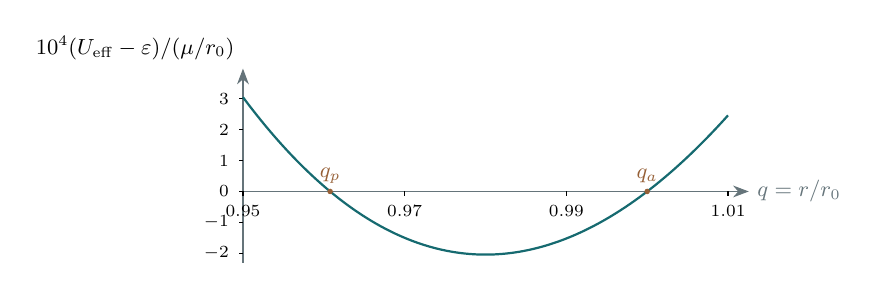
\begin{tikzpicture}[scale=.88,transform shape]
\draw[axis] (0,1.0267857142857144)--(7.3,1.0267857142857144) node[right] {$q=r/r_0$};
\draw[axis] (0,0)--(0,2.8);
\node[above left] at (0,2.8) {$10^4(U_{\rm eff}-\varepsilon)/(\mu/r_0)$};
\draw[thin] (0.000000,1.0267857142857144)--(0.000000,0.9667857142857144);\node[below,font=\scriptsize] at (0.000000,0.9467857142857145) {$ 0.95 $};
\draw[thin] (2.333333,1.0267857142857144)--(2.333333,0.9667857142857144);\node[below,font=\scriptsize] at (2.333333,0.9467857142857145) {$ 0.97 $};
\draw[thin] (4.666667,1.0267857142857144)--(4.666667,0.9667857142857144);\node[below,font=\scriptsize] at (4.666667,0.9467857142857145) {$ 0.99 $};
\draw[thin] (7.000000,1.0267857142857144)--(7.000000,0.9667857142857144);\node[below,font=\scriptsize] at (7.000000,0.9467857142857145) {$ 1.01 $};
\draw[thin] (0,0.133929)--(-.06,0.133929);\node[left,font=\scriptsize] at (-.08,0.133929) {$ -2 $};
\draw[thin] (0,0.580357)--(-.06,0.580357);\node[left,font=\scriptsize] at (-.08,0.580357) {$ -1 $};
\draw[thin] (0,1.026786)--(-.06,1.026786);\node[left,font=\scriptsize] at (-.08,1.026786) {$ 0 $};
\draw[thin] (0,1.473214)--(-.06,1.473214);\node[left,font=\scriptsize] at (-.08,1.473214) {$ 1 $};
\draw[thin] (0,1.919643)--(-.06,1.919643);\node[left,font=\scriptsize] at (-.08,1.919643) {$ 2 $};
\draw[thin] (0,2.366071)--(-.06,2.366071);\node[left,font=\scriptsize] at (-.08,2.366071) {$ 3 $};
\draw[thick,color=accent] plot coordinates {(0.0000000,2.3870944) (0.0291667,2.3482205) (0.0583333,2.3097023) (0.0875000,2.2715393) (0.1166667,2.2337310) (0.1458333,2.1962767) (0.1750000,2.1591760) (0.2041667,2.1224282) (0.2333333,2.0860329) (0.2625000,2.0499896) (0.2916667,2.0142976) (0.3208333,1.9789565) (0.3500000,1.9439656) (0.3791667,1.9093246) (0.4083333,1.8750328) (0.4375000,1.8410896) (0.4666667,1.8074947) (0.4958333,1.7742473) (0.5250000,1.7413471) (0.5541667,1.7087934) (0.5833333,1.6765858) (0.6125000,1.6447237) (0.6416667,1.6132065) (0.6708333,1.5820338) (0.7000000,1.5512051) (0.7291667,1.5207197) (0.7583333,1.4905772) (0.7875000,1.4607770) (0.8166667,1.4313186) (0.8458333,1.4022016) (0.8750000,1.3734253) (0.9041667,1.3449893) (0.9333333,1.3168930) (0.9625000,1.2891359) (0.9916667,1.2617175) (1.0208333,1.2346373) (1.0500000,1.2078947) (1.0791667,1.1814893) (1.1083333,1.1554205) (1.1375000,1.1296878) (1.1666667,1.1042907) (1.1958333,1.0792286) (1.2250000,1.0545012) (1.2541667,1.0301078) (1.2833333,1.0060479) (1.3125000,0.9823211) (1.3416667,0.9589268) (1.3708333,0.9358645) (1.4000000,0.9131337) (1.4291667,0.8907339) (1.4583333,0.8686646) (1.4875000,0.8469253) (1.5166667,0.8255155) (1.5458333,0.8044346) (1.5750000,0.7836822) (1.6041667,0.7632578) (1.6333333,0.7431609) (1.6625000,0.7233909) (1.6916667,0.7039474) (1.7208333,0.6848298) (1.7500000,0.6660378) (1.7791667,0.6475707) (1.8083333,0.6294280) (1.8375000,0.6116094) (1.8666667,0.5941142) (1.8958333,0.5769420) (1.9250000,0.5600923) (1.9541667,0.5435647) (1.9833333,0.5273585) (2.0125000,0.5114733) (2.0416667,0.4959086) (2.0708333,0.4806640) (2.1000000,0.4657389) (2.1291667,0.4511329) (2.1583333,0.4368455) (2.1875000,0.4228761) (2.2166667,0.4092243) (2.2458333,0.3958896) (2.2750000,0.3828716) (2.3041667,0.3701697) (2.3333333,0.3577834) (2.3625000,0.3457123) (2.3916667,0.3339559) (2.4208333,0.3225137) (2.4500000,0.3113852) (2.4791667,0.3005700) (2.5083333,0.2900675) (2.5375000,0.2798773) (2.5666667,0.2699990) (2.5958333,0.2604319) (2.6250000,0.2511758) (2.6541667,0.2422300) (2.6833333,0.2335941) (2.7125000,0.2252677) (2.7416667,0.2172502) (2.7708333,0.2095412) (2.8000000,0.2021402) (2.8291667,0.1950467) (2.8583333,0.1882604) (2.8875000,0.1817806) (2.9166667,0.1756070) (2.9458333,0.1697390) (2.9750000,0.1641763) (3.0041667,0.1589182) (3.0333333,0.1539645) (3.0625000,0.1493145) (3.0916667,0.1449679) (3.1208333,0.1409241) (3.1500000,0.1371828) (3.1791667,0.1337434) (3.2083333,0.1306055) (3.2375000,0.1277686) (3.2666667,0.1252323) (3.2958333,0.1229961) (3.3250000,0.1210595) (3.3541667,0.1194221) (3.3833333,0.1180835) (3.4125000,0.1170431) (3.4416667,0.1163005) (3.4708333,0.1158553) (3.5000000,0.1157070) (3.5291667,0.1158551) (3.5583333,0.1162993) (3.5875000,0.1170390) (3.6166667,0.1180738) (3.6458333,0.1194032) (3.6750000,0.1210268) (3.7041667,0.1229442) (3.7333333,0.1251548) (3.7625000,0.1276583) (3.7916667,0.1304542) (3.8208333,0.1335421) (3.8500000,0.1369214) (3.8791667,0.1405918) (3.9083333,0.1445528) (3.9375000,0.1488040) (3.9666667,0.1533449) (3.9958333,0.1581751) (4.0250000,0.1632941) (4.0541667,0.1687015) (4.0833333,0.1743969) (4.1125000,0.1803798) (4.1416667,0.1866497) (4.1708333,0.1932063) (4.2000000,0.2000491) (4.2291667,0.2071777) (4.2583333,0.2145915) (4.2875000,0.2222903) (4.3166667,0.2302735) (4.3458333,0.2385407) (4.3750000,0.2470915) (4.4041667,0.2559255) (4.4333333,0.2650421) (4.4625000,0.2744411) (4.4916667,0.2841219) (4.5208333,0.2940841) (4.5500000,0.3043273) (4.5791667,0.3148510) (4.6083333,0.3256549) (4.6375000,0.3367385) (4.6666667,0.3481013) (4.6958333,0.3597430) (4.7250000,0.3716631) (4.7541667,0.3838612) (4.7833333,0.3963369) (4.8125000,0.4090897) (4.8416667,0.4221193) (4.8708333,0.4354251) (4.9000000,0.4490068) (4.9291667,0.4628640) (4.9583333,0.4769961) (4.9875000,0.4914029) (5.0166667,0.5060839) (5.0458333,0.5210386) (5.0750000,0.5362667) (5.1041667,0.5517678) (5.1333333,0.5675413) (5.1625000,0.5835870) (5.1916667,0.5999043) (5.2208333,0.6164929) (5.2500000,0.6333523) (5.2791667,0.6504822) (5.3083333,0.6678820) (5.3375000,0.6855515) (5.3666667,0.7034902) (5.3958333,0.7216977) (5.4250000,0.7401736) (5.4541667,0.7589174) (5.4833333,0.7779287) (5.5125000,0.7972072) (5.5416667,0.8167525) (5.5708333,0.8365641) (5.6000000,0.8566415) (5.6291667,0.8769845) (5.6583333,0.8975926) (5.6875000,0.9184654) (5.7166667,0.9396025) (5.7458333,0.9610035) (5.7750000,0.9826679) (5.8041667,1.0045955) (5.8333333,1.0267857) (5.8625000,1.0492382) (5.8916667,1.0719526) (5.9208333,1.0949284) (5.9500000,1.1181654) (5.9791667,1.1416630) (6.0083333,1.1654208) (6.0375000,1.1894386) (6.0666667,1.2137158) (6.0958333,1.2382521) (6.1250000,1.2630471) (6.1541667,1.2881004) (6.1833333,1.3134116) (6.2125000,1.3389803) (6.2416667,1.3648061) (6.2708333,1.3908886) (6.3000000,1.4172274) (6.3291667,1.4438221) (6.3583333,1.4706724) (6.3875000,1.4977778) (6.4166667,1.5251379) (6.4458333,1.5527525) (6.4750000,1.5806210) (6.5041667,1.6087430) (6.5333333,1.6371183) (6.5625000,1.6657464) (6.5916667,1.6946269) (6.6208333,1.7237594) (6.6500000,1.7531436) (6.6791667,1.7827791) (6.7083333,1.8126654) (6.7375000,1.8428022) (6.7666667,1.8731891) (6.7958333,1.9038257) (6.8250000,1.9347117) (6.8541667,1.9658467) (6.8833333,1.9972302) (6.9125000,2.0288619) (6.9416667,2.0607414) (6.9708333,2.0928684) (7.0000000,2.1252424)};
\fill[color=warm] (1.2581699,1.0267857) circle(.04) node[above] {$q_p$};
\fill[color=warm] (5.8333333,1.0267857) circle(.04) node[above] {$q_a$};
\end{tikzpicture}
\figcaption{解图力试1.5B\quad 实际2\%动能损失下，两个零点给径向转折半径}
\end{minipage}\end{center}
解图力试1.5B用有效势把远、近两个转折点标出来。碰撞之后单位质量角动量$j=r_0v_+=r_pv_p$守恒，故$v_p/v_+=r_0/r_p=51/49$；图A的近地点速度较大。径向能量方程为
\[
\frac12\dot r^2+\frac{j^2}{2r^2}-\frac{\mu}{r}
=\varepsilon,\qquad
j^2=0.98\,\mu r_0.
\]
转折点满足$\dot r=0$。取$q=r/r_0$，代入得到
\[
1.02q^2-2q+0.98=0
\ \Longleftrightarrow\
(q-1)(1.02q-0.98)=0.
\]
两根恰为$r_a/r_0=1$和$r_p/r_0=0.98/1.02$，与前面的椭圆长轴关系给出同一对端点。新轨道偏心率为
\[
e=\frac{r_a-r_p}{r_a+r_p}=0.02.
\]
解图力试1.5A按$e=0.02$画出实际椭圆，地心与几何中心只有较小的偏移。碰撞阶段能量、角动量会改变；这些守恒关系只从碰撞结束后开始使用。

同一推导若把切向动能损失比例写成$\delta$，便有$\varepsilon=-(1+\delta)\mu/(2r_0)$、$a_o=r_0/(1+\delta)$及$r_p/r_0=(1-\delta)/(1+\delta)$。解图力试1.5C画这一连续关系，2\%损失对应近地点半径约为初始半径的0.960784。
\begin{center}\begin{minipage}{.98\linewidth}\centering
\begin{tikzpicture}[scale=.88,transform shape]
\draw[axis] (0,0)--(7.3,0) node[right] {$\delta$};
\draw[axis] (0,0)--(0,2.8);
\node[above left] at (0,2.8) {$r_p/r_0$};
\draw[thin] (0.000000,0)--(0.000000,-0.06);\node[below,font=\scriptsize] at (0.000000,-0.08) {$ 0 $};
\draw[thin] (0.583333,0)--(0.583333,-0.06);\node[below,font=\scriptsize] at (0.583333,-0.08) {$ 0.02 $};
\draw[thin] (2.333333,0)--(2.333333,-0.06);\node[below,font=\scriptsize] at (2.333333,-0.08) {$ 0.08 $};
\draw[thin] (4.666667,0)--(4.666667,-0.06);\node[below,font=\scriptsize] at (4.666667,-0.08) {$ 0.16 $};
\draw[thin] (7.000000,0)--(7.000000,-0.06);\node[below,font=\scriptsize] at (7.000000,-0.08) {$ 0.24 $};
\draw[thin] (0,0.000000)--(-.06,0.000000);\node[left,font=\scriptsize] at (-.08,0.000000) {$ 0.6 $};
\draw[thin] (0,1.111111)--(-.06,1.111111);\node[left,font=\scriptsize] at (-.08,1.111111) {$ 0.8 $};
\draw[thin] (0,2.222222)--(-.06,2.222222);\node[left,font=\scriptsize] at (-.08,2.222222) {$ 1 $};
\draw[thick,color=accent] plot coordinates {(0.0000000,2.2222222) (0.0291667,2.2111222) (0.0583333,2.2000444) (0.0875000,2.1889886) (0.1166667,2.1779548) (0.1458333,2.1669431) (0.1750000,2.1559532) (0.2041667,2.1449851) (0.2333333,2.1340388) (0.2625000,2.1231142) (0.2916667,2.1122112) (0.3208333,2.1013298) (0.3500000,2.0904699) (0.3791667,2.0796315) (0.4083333,2.0688144) (0.4375000,2.0580186) (0.4666667,2.0472441) (0.4958333,2.0364908) (0.5250000,2.0257586) (0.5541667,2.0150474) (0.5833333,2.0043573) (0.6125000,1.9936881) (0.6416667,1.9830398) (0.6708333,1.9724123) (0.7000000,1.9618056) (0.7291667,1.9512195) (0.7583333,1.9406541) (0.7875000,1.9301093) (0.8166667,1.9195850) (0.8458333,1.9090811) (0.8750000,1.8985976) (0.9041667,1.8881345) (0.9333333,1.8776916) (0.9625000,1.8672690) (0.9916667,1.8568665) (1.0208333,1.8464842) (1.0500000,1.8361218) (1.0791667,1.8257795) (1.1083333,1.8154571) (1.1375000,1.8051545) (1.1666667,1.7948718) (1.1958333,1.7846088) (1.2250000,1.7743655) (1.2541667,1.7641419) (1.2833333,1.7539378) (1.3125000,1.7437533) (1.3416667,1.7335883) (1.3708333,1.7234426) (1.4000000,1.7133164) (1.4291667,1.7032094) (1.4583333,1.6931217) (1.4875000,1.6830532) (1.5166667,1.6730038) (1.5458333,1.6629735) (1.5750000,1.6529623) (1.6041667,1.6429700) (1.6333333,1.6329966) (1.6625000,1.6230422) (1.6916667,1.6131065) (1.7208333,1.6031896) (1.7500000,1.5932914) (1.7791667,1.5834119) (1.8083333,1.5735510) (1.8375000,1.5637086) (1.8666667,1.5538847) (1.8958333,1.5440793) (1.9250000,1.5342923) (1.9541667,1.5245236) (1.9833333,1.5147732) (2.0125000,1.5050411) (2.0416667,1.4953271) (2.0708333,1.4856313) (2.1000000,1.4759536) (2.1291667,1.4662939) (2.1583333,1.4566522) (2.1875000,1.4470284) (2.2166667,1.4374226) (2.2458333,1.4278345) (2.2750000,1.4182643) (2.3041667,1.4087118) (2.3333333,1.3991770) (2.3625000,1.3896598) (2.3916667,1.3801602) (2.4208333,1.3706782) (2.4500000,1.3612136) (2.4791667,1.3517665) (2.5083333,1.3423368) (2.5375000,1.3329245) (2.5666667,1.3235294) (2.5958333,1.3141516) (2.6250000,1.3047910) (2.6541667,1.2954476) (2.6833333,1.2861213) (2.7125000,1.2768120) (2.7416667,1.2675198) (2.7708333,1.2582445) (2.8000000,1.2489862) (2.8291667,1.2397448) (2.8583333,1.2305201) (2.8875000,1.2213123) (2.9166667,1.2121212) (2.9458333,1.2029468) (2.9750000,1.1937891) (3.0041667,1.1846479) (3.0333333,1.1755233) (3.0625000,1.1664153) (3.0916667,1.1573237) (3.1208333,1.1482485) (3.1500000,1.1391897) (3.1791667,1.1301473) (3.2083333,1.1211211) (3.2375000,1.1121112) (3.2666667,1.1031175) (3.2958333,1.0941400) (3.3250000,1.0851785) (3.3541667,1.0762332) (3.3833333,1.0673039) (3.4125000,1.0583905) (3.4416667,1.0494931) (3.4708333,1.0406117) (3.5000000,1.0317460) (3.5291667,1.0228962) (3.5583333,1.0140622) (3.5875000,1.0052439) (3.6166667,0.9964413) (3.6458333,0.9876543) (3.6750000,0.9788830) (3.7041667,0.9701272) (3.7333333,0.9613869) (3.7625000,0.9526621) (3.7916667,0.9439528) (3.8208333,0.9352589) (3.8500000,0.9265803) (3.8791667,0.9179170) (3.9083333,0.9092691) (3.9375000,0.9006363) (3.9666667,0.8920188) (3.9958333,0.8834164) (4.0250000,0.8748291) (4.0541667,0.8662570) (4.0833333,0.8576998) (4.1125000,0.8491577) (4.1416667,0.8406305) (4.1708333,0.8321182) (4.2000000,0.8236208) (4.2291667,0.8151383) (4.2583333,0.8066705) (4.2875000,0.7982176) (4.3166667,0.7897793) (4.3458333,0.7813558) (4.3750000,0.7729469) (4.4041667,0.7645526) (4.4333333,0.7561728) (4.4625000,0.7478077) (4.4916667,0.7394570) (4.5208333,0.7311207) (4.5500000,0.7227989) (4.5791667,0.7144915) (4.6083333,0.7061984) (4.6375000,0.6979197) (4.6666667,0.6896552) (4.6958333,0.6814049) (4.7250000,0.6731689) (4.7541667,0.6649470) (4.7833333,0.6567392) (4.8125000,0.6485455) (4.8416667,0.6403659) (4.8708333,0.6322003) (4.9000000,0.6240487) (4.9291667,0.6159110) (4.9583333,0.6077873) (4.9875000,0.5996774) (5.0166667,0.5915813) (5.0458333,0.5834991) (5.0750000,0.5754306) (5.1041667,0.5673759) (5.1333333,0.5593348) (5.1625000,0.5513075) (5.1916667,0.5432937) (5.2208333,0.5352936) (5.2500000,0.5273070) (5.2791667,0.5193339) (5.3083333,0.5113743) (5.3375000,0.5034282) (5.3666667,0.4954955) (5.3958333,0.4875762) (5.4250000,0.4796702) (5.4541667,0.4717776) (5.4833333,0.4638982) (5.5125000,0.4560321) (5.5416667,0.4481793) (5.5708333,0.4403396) (5.6000000,0.4325130) (5.6291667,0.4246996) (5.6583333,0.4168993) (5.6875000,0.4091120) (5.7166667,0.4013378) (5.7458333,0.3935765) (5.7750000,0.3858282) (5.8041667,0.3780929) (5.8333333,0.3703704) (5.8625000,0.3626607) (5.8916667,0.3549639) (5.9208333,0.3472799) (5.9500000,0.3396087) (5.9791667,0.3319502) (6.0083333,0.3243044) (6.0375000,0.3166713) (6.0666667,0.3090508) (6.0958333,0.3014429) (6.1250000,0.2938476) (6.1541667,0.2862648) (6.1833333,0.2786945) (6.2125000,0.2711368) (6.2416667,0.2635914) (6.2708333,0.2560585) (6.3000000,0.2485380) (6.3291667,0.2410299) (6.3583333,0.2335340) (6.3875000,0.2260505) (6.4166667,0.2185792) (6.4458333,0.2111202) (6.4750000,0.2036734) (6.5041667,0.1962388) (6.5333333,0.1888163) (6.5625000,0.1814059) (6.5916667,0.1740076) (6.6208333,0.1666214) (6.6500000,0.1592472) (6.6791667,0.1518850) (6.7083333,0.1445348) (6.7375000,0.1371965) (6.7666667,0.1298701) (6.7958333,0.1225556) (6.8250000,0.1152530) (6.8541667,0.1079622) (6.8833333,0.1006832) (6.9125000,0.0934160) (6.9416667,0.0861605) (6.9708333,0.0789167) (7.0000000,0.0716846)};
\end{tikzpicture}
\figcaption{解图力试1.5C\quad 切向动能损失增加使新近地点下降}
\end{minipage}\end{center}
从远地点开始计时，在点质量引力模型中轨道周期为 $T_o=2\pi\sqrt{a_o^3/\mu}$，到近地点用时 $T_o/2$。解图力试1.5D按 $2\%$ 的动能损失画出这半周：半径单调下降，在两个转折点的斜率为零。若地表半径介于 $r_p$ 和 $r_0$ 之间，图中下降段与地表半径线的首个交点给实际触地时刻。
\begin{center}\begin{minipage}{.98\linewidth}\centering
\begin{tikzpicture}[scale=.88,transform shape]
\draw[axis] (0,0)--(7.3,0) node[right] {$2t/T_o$};
\draw[axis] (0,0)--(0,2.8);
\node[above left] at (0,2.8) {$r/r_0$};
\draw[thin] (0.000000,0)--(0.000000,-0.06);\node[below,font=\scriptsize] at (0.000000,-0.08) {$ 0 $};
\draw[thin] (1.750000,0)--(1.750000,-0.06);\node[below,font=\scriptsize] at (1.750000,-0.08) {$ 0.25 $};
\draw[thin] (3.500000,0)--(3.500000,-0.06);\node[below,font=\scriptsize] at (3.500000,-0.08) {$ 0.5 $};
\draw[thin] (5.250000,0)--(5.250000,-0.06);\node[below,font=\scriptsize] at (5.250000,-0.08) {$ 0.75 $};
\draw[thin] (7.000000,0)--(7.000000,-0.06);\node[below,font=\scriptsize] at (7.000000,-0.08) {$ 1 $};
\draw[thin] (0,0.454545)--(-.06,0.454545);\node[left,font=\scriptsize] at (-.08,0.454545) {$ 0.96 $};
\draw[thin] (0,1.363636)--(-.06,1.363636);\node[left,font=\scriptsize] at (-.08,1.363636) {$ 0.98 $};
\draw[thin] (0,2.272727)--(-.06,2.272727);\node[left,font=\scriptsize] at (-.08,2.272727) {$ 1 $};
\draw[thick,color=accent] plot coordinates {(0.0000000,2.2727273) (0.0291667,2.2726539) (0.0583333,2.2724337) (0.0875000,2.2720668) (0.1166667,2.2715532) (0.1458333,2.2708930) (0.1750000,2.2700863) (0.2041667,2.2691332) (0.2333333,2.2680339) (0.2625000,2.2667885) (0.2916667,2.2653973) (0.3208333,2.2638603) (0.3500000,2.2621779) (0.3791667,2.2603504) (0.4083333,2.2583779) (0.4375000,2.2562608) (0.4666667,2.2539995) (0.4958333,2.2515942) (0.5250000,2.2490453) (0.5541667,2.2463533) (0.5833333,2.2435185) (0.6125000,2.2405413) (0.6416667,2.2374222) (0.6708333,2.2341618) (0.7000000,2.2307604) (0.7291667,2.2272186) (0.7583333,2.2235370) (0.7875000,2.2197161) (0.8166667,2.2157564) (0.8458333,2.2116587) (0.8750000,2.2074235) (0.9041667,2.2030514) (0.9333333,2.1985432) (0.9625000,2.1938996) (0.9916667,2.1891211) (1.0208333,2.1842087) (1.0500000,2.1791630) (1.0791667,2.1739847) (1.1083333,2.1686748) (1.1375000,2.1632340) (1.1666667,2.1576632) (1.1958333,2.1519632) (1.2250000,2.1461349) (1.2541667,2.1401792) (1.2833333,2.1340969) (1.3125000,2.1278892) (1.3416667,2.1215568) (1.3708333,2.1151009) (1.4000000,2.1085223) (1.4291667,2.1018222) (1.4583333,2.0950015) (1.4875000,2.0880614) (1.5166667,2.0810028) (1.5458333,2.0738269) (1.5750000,2.0665349) (1.6041667,2.0591278) (1.6333333,2.0516068) (1.6625000,2.0439730) (1.6916667,2.0362278) (1.7208333,2.0283722) (1.7500000,2.0204076) (1.7791667,2.0123351) (1.8083333,2.0041561) (1.8375000,1.9958718) (1.8666667,1.9874835) (1.8958333,1.9789926) (1.9250000,1.9704004) (1.9541667,1.9617082) (1.9833333,1.9529174) (2.0125000,1.9440295) (2.0416667,1.9350458) (2.0708333,1.9259677) (2.1000000,1.9167968) (2.1291667,1.9075344) (2.1583333,1.8981820) (2.1875000,1.8887411) (2.2166667,1.8792133) (2.2458333,1.8696000) (2.2750000,1.8599028) (2.3041667,1.8501233) (2.3333333,1.8402630) (2.3625000,1.8303235) (2.3916667,1.8203064) (2.4208333,1.8102133) (2.4500000,1.8000459) (2.4791667,1.7898057) (2.5083333,1.7794945) (2.5375000,1.7691139) (2.5666667,1.7586657) (2.5958333,1.7481514) (2.6250000,1.7375728) (2.6541667,1.7269317) (2.6833333,1.7162298) (2.7125000,1.7054688) (2.7416667,1.6946505) (2.7708333,1.6837766) (2.8000000,1.6728490) (2.8291667,1.6618694) (2.8583333,1.6508397) (2.8875000,1.6397617) (2.9166667,1.6286371) (2.9458333,1.6174679) (2.9750000,1.6062559) (3.0041667,1.5950030) (3.0333333,1.5837109) (3.0625000,1.5723817) (3.0916667,1.5610171) (3.1208333,1.5496192) (3.1500000,1.5381897) (3.1791667,1.5267306) (3.2083333,1.5152439) (3.2375000,1.5037314) (3.2666667,1.4921951) (3.2958333,1.4806369) (3.3250000,1.4690589) (3.3541667,1.4574628) (3.3833333,1.4458508) (3.4125000,1.4342248) (3.4416667,1.4225867) (3.4708333,1.4109385) (3.5000000,1.3992822) (3.5291667,1.3876199) (3.5583333,1.3759534) (3.5875000,1.3642848) (3.6166667,1.3526161) (3.6458333,1.3409493) (3.6750000,1.3292864) (3.7041667,1.3176294) (3.7333333,1.3059804) (3.7625000,1.2943412) (3.7916667,1.2827140) (3.8208333,1.2711008) (3.8500000,1.2595035) (3.8791667,1.2479242) (3.9083333,1.2363649) (3.9375000,1.2248277) (3.9666667,1.2133145) (3.9958333,1.2018273) (4.0250000,1.1903682) (4.0541667,1.1789392) (4.0833333,1.1675422) (4.1125000,1.1561794) (4.1416667,1.1448526) (4.1708333,1.1335639) (4.2000000,1.1223153) (4.2291667,1.1111088) (4.2583333,1.0999464) (4.2875000,1.0888300) (4.3166667,1.0777616) (4.3458333,1.0667433) (4.3750000,1.0557769) (4.4041667,1.0448644) (4.4333333,1.0340078) (4.4625000,1.0232090) (4.4916667,1.0124700) (4.5208333,1.0017927) (4.5500000,0.9911789) (4.5791667,0.9806307) (4.6083333,0.9701500) (4.6375000,0.9597385) (4.6666667,0.9493983) (4.6958333,0.9391312) (4.7250000,0.9289390) (4.7541667,0.9188236) (4.7833333,0.9087868) (4.8125000,0.8988305) (4.8416667,0.8889565) (4.8708333,0.8791666) (4.9000000,0.8694626) (4.9291667,0.8598462) (4.9583333,0.8503193) (4.9875000,0.8408835) (5.0166667,0.8315407) (5.0458333,0.8222924) (5.0750000,0.8131405) (5.1041667,0.8040867) (5.1333333,0.7951325) (5.1625000,0.7862797) (5.1916667,0.7775299) (5.2208333,0.7688848) (5.2500000,0.7603458) (5.2791667,0.7519147) (5.3083333,0.7435929) (5.3375000,0.7353821) (5.3666667,0.7272838) (5.3958333,0.7192994) (5.4250000,0.7114306) (5.4541667,0.7036786) (5.4833333,0.6960451) (5.5125000,0.6885314) (5.5416667,0.6811389) (5.5708333,0.6738691) (5.6000000,0.6667233) (5.6291667,0.6597028) (5.6583333,0.6528090) (5.6875000,0.6460432) (5.7166667,0.6394066) (5.7458333,0.6329006) (5.7750000,0.6265262) (5.8041667,0.6202848) (5.8333333,0.6141775) (5.8625000,0.6082056) (5.8916667,0.6023700) (5.9208333,0.5966719) (5.9500000,0.5911125) (5.9791667,0.5856928) (6.0083333,0.5804137) (6.0375000,0.5752763) (6.0666667,0.5702817) (6.0958333,0.5654306) (6.1250000,0.5607242) (6.1541667,0.5561632) (6.1833333,0.5517485) (6.2125000,0.5474810) (6.2416667,0.5433615) (6.2708333,0.5393908) (6.3000000,0.5355697) (6.3291667,0.5318988) (6.3583333,0.5283789) (6.3875000,0.5250107) (6.4166667,0.5217948) (6.4458333,0.5187318) (6.4750000,0.5158223) (6.5041667,0.5130669) (6.5333333,0.5104661) (6.5625000,0.5080204) (6.5916667,0.5057303) (6.6208333,0.5035962) (6.6500000,0.5016185) (6.6791667,0.4997977) (6.7083333,0.4981339) (6.7375000,0.4966277) (6.7666667,0.4952793) (6.7958333,0.4940888) (6.8250000,0.4930567) (6.8541667,0.4921829) (6.8833333,0.4914679) (6.9125000,0.4909115) (6.9416667,0.4905141) (6.9708333,0.4902756) (7.0000000,0.4901961)};
\end{tikzpicture}
\figcaption{解图力试1.5D\quad 实际轨道从远地点到近地点的半周径向过程}
\end{minipage}\end{center}


\Needspace{13\baselineskip}

\pdfbookmark[2]{第 6 题 绳杆受冲量后的初动与摆角条件}{q6}

\section*{第 6 题\quad 绳杆受冲量后的初动与摆角条件}\label{q:6}


均匀细杆质量为$M$、长度为$2L$，由长为$l$的轻绳竖直悬挂，绳上端固定在$P$，下端接杆的上端$A$。系统起初静止。给杆下端$B$一个水平向右、持续时间极短的冲量$J$。
\begin{enumerate}
\item 画出刚开始运动时绳与杆的偏转方向。
\item 求冲量结束瞬间绳角速度$\dot\theta(0^+)$与杆角速度$\dot\varphi(0^+)$。两角都从竖直向下方向量起，向右偏为正。
\item 建立摆角与能量的关系，说明在所谓“最大摆角”时可使用什么条件；区分单个角达到极值和绳、杆同时瞬时静止。
\end{enumerate}
杆可绕绳杆连接点在竖直平面内摆动，忽略阻力。涉及后续约束运动的公式用于绳保持张紧的阶段。


\begin{center}\begin{minipage}{.98\linewidth}\centering
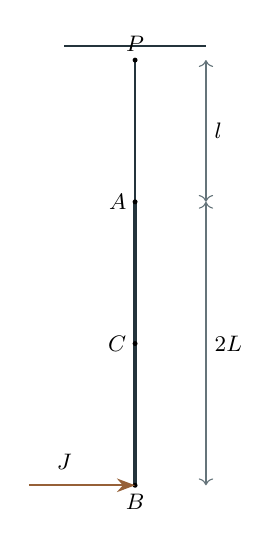
\begin{tikzpicture}[scale=.9,transform shape]
\draw[object] (-1.00000,0.20000)--(1.00000,0.20000);\draw[object] (0.00000,0.00000)--(0.00000,-2.00000);\draw[very thick,color=ink] (0.00000,-2.00000)--(0.00000,-6.00000);\fill (0.00000,0.00000) circle(.035);\node[above] at (0.00000,0.00000) {$P$};\fill (0.00000,-2.00000) circle(.035);\node[left] at (0.00000,-2.00000) {$A$};\fill (0.00000,-4.00000) circle(.035);\node[left] at (0.00000,-4.00000) {$C$};\fill (0.00000,-6.00000) circle(.035);\node[below] at (0.00000,-6.00000) {$B$};\draw[force] (-1.50000,-6.00000)--(0.00000,-6.00000);\node[above] at (-1.00000,-5.90000) {$J$};\draw[<->,thin,color=muted] (1.00000,0.00000)--(1.00000,-2.00000);\node[right] at (1.00000,-1.00000) {$l$};\draw[<->,thin,color=muted] (1.00000,-2.00000)--(1.00000,-6.00000);\node[right] at (1.00000,-4.00000) {$2L$};
\end{tikzpicture}
\figcaption{图力试1.6\quad 竖直绳杆，水平冲量施加在杆下端B。}
\end{minipage}\end{center}

\Needspace{6\baselineskip}\subsection*{解答}


图力试1.6的初始状态中，杆质心$C$在$A$下方$L$处。冲量作用时间极短，重力冲量可略；轻绳沿竖直方向，对杆没有水平冲量。因此
\[
MV_C=J,\qquad V_C=\frac JM.
\]
给杆关于自身质心的转动冲量为$JL$，杆的质心惯量$I_C=ML^2/3$，所以
\[
I_C\dot\varphi=JL,\qquad
\boxed{\dot\varphi(0^+)=\frac{3J}{ML}>0}.
\]

\begin{center}\begin{minipage}{.98\linewidth}\centering
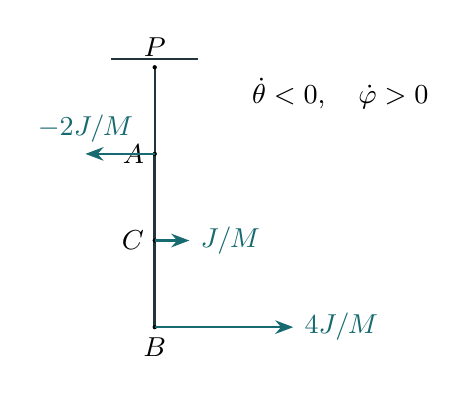
\begin{tikzpicture}[scale=1.1,transform shape]
\draw[object] (-.5,.1)--(.5,.1);\draw[object] (0,0)--(0,-1);\draw[very thick,color=ink] (0,-1)--(0,-3);
\fill (0,0) circle(.025) node[above] {$P$};\fill (0,-1) circle(.025) node[left] {$A$};\fill (0,-2) circle(.025) node[left] {$C$};\fill (0,-3) circle(.025) node[below] {$B$};
\draw[motion] (0,-1)--(-.8,-1) node[above] {$-2J/M$};\draw[motion] (0,-2)--(.4,-2) node[right] {$J/M$};\draw[motion] (0,-3)--(1.6,-3) node[right] {$4J/M$};
\node[right] at (1,-.3) {$\dot\theta<0,\quad\dot\varphi>0$};
\end{tikzpicture}
\figcaption{解图力试1.6A\quad 初始速度场：上端向左，质心与下端向右}
\end{minipage}\end{center}
（1）解图力试1.6A的速度箭头由质心平移和绕质心转动相加。杆上端和下端的初速度分别为
\[
V_A=V_C-L\dot\varphi=-\frac{2J}{M},
\qquad
V_B=V_C+L\dot\varphi=\frac{4J}{M}.
\]
所以杆上端先向左，下端向右；轻绳开始向左偏，细杆开始向右偏。下端冲量与绕质心转动共同决定两端速度，上端反向使绳角先取负值。

（2）冲量结束瞬间轻绳仍竖直，连接点$A$的速度满足$V_A=l\dot\theta$，故
\[
\boxed{\dot\theta(0^+)=-\frac{2J}{Ml},\qquad
\dot\varphi(0^+)=\frac{3J}{ML}}.
\]
在杆上还可找瞬心$O$：由$V_C=\dot\varphi\,OC$得
\[
OC=\frac L3,
\]
位于质心上方，即距杆下端$4L/3$。解图力试1.6B只表示这一瞬间的速度场；$O$按初始速度场定义，后续位置随运动状态确定。

若直接对初始瞬心求角冲量，记$x=OC$，平行轴定理给$I_O=ML^2/3+Mx^2$，而$J=M\dot\varphi x$。代入$J(L+x)=I_O\dot\varphi$，消去冲量和角速度后得到$x(L+x)=L^2/3+x^2$，即$x=L/3$。它与前面质心平移、转动得到同一初始速度场。初始无穷小位移有$\dd\varphi=-3l\,\dd\theta/(2L)$，同样体现绳左偏、杆右偏的方向。

\begin{center}\begin{minipage}{.98\linewidth}\centering
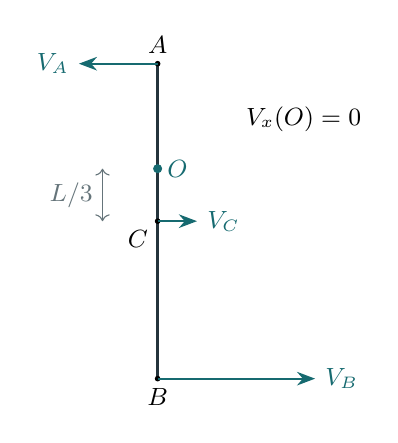
\begin{tikzpicture}[scale=2]
\draw[very thick,color=ink] (0,-1)--(0,1);
\fill (0,1) circle(.018) node[above] {$A$};\fill (0,0) circle(.018) node[below left] {$C$};\fill (0,-1) circle(.018) node[below] {$B$};
\draw[fill=white,color=accent] (0,.3333333) circle(.025) node[right] {$O$};
\draw[<->,thin,color=muted] (-.35,0)--(-.35,.3333333) node[midway,left] {$L/3$};
\draw[motion] (0,1)--(-.5,1) node[left] {$V_A$};\draw[motion] (0,0)--(.25,0) node[right] {$V_C$};\draw[motion] (0,-1)--(1,-1) node[right] {$V_B$};
\node[right] at (.5,.65) {$V_x(O)=0$};
\end{tikzpicture}
\figcaption{解图力试1.6B\quad 初始竖直杆的瞬心在C上方，$OC=L/3$}
\end{minipage}\end{center}

（3）刚受冲量后的总动能为
\[
K_0=\frac12MV_C^2+\frac12I_C\dot\varphi^2
=\frac{J^2}{2M}+\frac{3J^2}{2M}
=\boxed{\frac{2J^2}{M}}.
\]
取初始重力势能为零。任意张紧状态中
\[
x_C=l\sin\theta+L\sin\varphi,\quad
y_C=-l\cos\theta-L\cos\varphi.
\]
对坐标求导并加上杆绕质心转动能，得
\[
K=\frac M2\left[
l^2\dot\theta^2+\frac{4L^2}{3}\dot\varphi^2
+2lL\cos(\theta-\varphi)\dot\theta\dot\varphi
\right],
\]
\[
U=Mg\left[l(1-\cos\theta)+L(1-\cos\varphi)\right],
\qquad \boxed{K+U=\frac{2J^2}{M}}.
\]
质量矩阵的行列式为$l^2L^2[4/3-\cos^2(\theta-\varphi)]>0$，所以$K=0$当且仅当$\dot\theta=\dot\varphi=0$。


由完整动能和势能作Lagrange运算，张紧阶段的运动方程为
\[
 \begin{aligned}
 l^2\ddot\theta+lL\cos(\theta-\varphi)\ddot\varphi
  +lL\sin(\theta-\varphi)\dot\varphi^2+gl\sin\theta&=0,\\
 lL\cos(\theta-\varphi)\ddot\theta+\frac{4L^2}{3}\ddot\varphi
  -lL\sin(\theta-\varphi)\dot\theta^2+gL\sin\varphi&=0 .
 \end{aligned}
\]
其初值为$\theta=\varphi=0$和上列两个角速度。绳拉力由质心沿绳方向的受力求出，
\[
 T=M\left[g\cos\theta+l\dot\theta^2
 -L\ddot\varphi\sin(\theta-\varphi)
 +L\dot\varphi^2\cos(\theta-\varphi)\right].
\]
正拉力与定绳长约束共同给出张紧运动段。

\begin{center}\begin{minipage}{.98\linewidth}\centering
\begin{tikzpicture}[scale=.85,transform shape]
\draw[axis] (-3.4,0)--(3.5,0) node[right] {$\theta/\mathrm{rad}$};\draw[axis] (0,-3.4)--(0,3.5) node[above] {$\varphi/\mathrm{rad}$};
\foreach \p/\q in {-3/-.4,-1.5/-.2,1.5/.2,3/.4}{
\draw[thin] (\p,0)--(\p,-.06) node[below,font=\scriptsize] {$\q$};
\draw[thin] (0,\p)--(-.06,\p) node[left,font=\scriptsize] {$\q$};}
\node[below right,font=\scriptsize] at (0,0) {$0$};
\draw[thick,color=accent] plot coordinates {(-3.0203688,0.0000001) (-2.9951991,0.3839483) (-2.9700293,0.5419675) (-2.9448596,0.6625210) (-2.9196899,0.7635636) (-2.8945201,0.8520631) (-2.8693504,0.9315994) (-2.8441806,1.0043028) (-2.8190109,1.0715636) (-2.7938412,1.1343491) (-2.7686714,1.1933645) (-2.7435017,1.2491432) (-2.7183319,1.3021001) (-2.6931622,1.3525655) (-2.6679925,1.4008079) (-2.6428227,1.4470484) (-2.6176530,1.4914724) (-2.5924832,1.5342368) (-2.5673135,1.5754758) (-2.5421437,1.6153053) (-2.5169740,1.6538265) (-2.4918043,1.6911279) (-2.4666345,1.7272878) (-2.4414648,1.7623755) (-2.4162950,1.7964534) (-2.3911253,1.8295769) (-2.3659556,1.8617965) (-2.3407858,1.8931574) (-2.3156161,1.9237012) (-2.2904463,1.9534654) (-2.2652766,1.9824845) (-2.2401069,2.0107902) (-2.2149371,2.0384116) (-2.1897674,2.0653755) (-2.1645976,2.0917067) (-2.1394279,2.1174284) (-2.1142582,2.1425619) (-2.0890884,2.1671271) (-2.0639187,2.1911427) (-2.0387489,2.2146259) (-2.0135792,2.2375930) (-1.9884095,2.2600593) (-1.9632397,2.2820391) (-1.9380700,2.3035457) (-1.9129002,2.3245919) (-1.8877305,2.3451896) (-1.8625608,2.3653501) (-1.8373910,2.3850840) (-1.8122213,2.4044014) (-1.7870515,2.4233117) (-1.7618818,2.4418242) (-1.7367121,2.4599472) (-1.7115423,2.4776891) (-1.6863726,2.4950574) (-1.6612028,2.5120596) (-1.6360331,2.5287027) (-1.6108634,2.5449934) (-1.5856936,2.5609380) (-1.5605239,2.5765426) (-1.5353541,2.5918130) (-1.5101844,2.6067547) (-1.4850147,2.6213730) (-1.4598449,2.6356730) (-1.4346752,2.6496594) (-1.4095054,2.6633371) (-1.3843357,2.6767102) (-1.3591660,2.6897832) (-1.3339962,2.7025600) (-1.3088265,2.7150445) (-1.2836567,2.7272406) (-1.2584870,2.7391517) (-1.2333173,2.7507813) (-1.2081475,2.7621328) (-1.1829778,2.7732091) (-1.1578080,2.7840135) (-1.1326383,2.7945488) (-1.1074686,2.8048177) (-1.0822988,2.8148231) (-1.0571291,2.8245673) (-1.0319593,2.8340531) (-1.0067896,2.8432826) (-0.9816199,2.8522582) (-0.9564501,2.8609820) (-0.9312804,2.8694562) (-0.9061106,2.8776828) (-0.8809409,2.8856637) (-0.8557712,2.8934008) (-0.8306014,2.9008958) (-0.8054317,2.9081504) (-0.7802619,2.9151663) (-0.7550922,2.9219450) (-0.7299225,2.9284880) (-0.7047527,2.9347968) (-0.6795830,2.9408727) (-0.6544132,2.9467170) (-0.6292435,2.9523309) (-0.6040738,2.9577157) (-0.5789040,2.9628725) (-0.5537343,2.9678022) (-0.5285645,2.9725061) (-0.5033948,2.9769849) (-0.4782251,2.9812397) (-0.4530553,2.9852712) (-0.4278856,2.9890804) (-0.4027158,2.9926679) (-0.3775461,2.9960345) (-0.3523764,2.9991808) (-0.3272066,3.0021075) (-0.3020369,3.0048151) (-0.2768671,3.0073042) (-0.2516974,3.0095753) (-0.2265277,3.0116287) (-0.2013579,3.0134649) (-0.1761882,3.0150843) (-0.1510184,3.0164871) (-0.1258487,3.0176737) (-0.1006790,3.0186442) (-0.0755092,3.0193988) (-0.0503395,3.0199377) (-0.0251697,3.0202610) (0.0000000,3.0203688) (0.0251697,3.0202610) (0.0503395,3.0199377) (0.0755092,3.0193988) (0.1006790,3.0186442) (0.1258487,3.0176737) (0.1510184,3.0164871) (0.1761882,3.0150843) (0.2013579,3.0134649) (0.2265277,3.0116287) (0.2516974,3.0095753) (0.2768671,3.0073042) (0.3020369,3.0048151) (0.3272066,3.0021075) (0.3523764,2.9991808) (0.3775461,2.9960345) (0.4027158,2.9926679) (0.4278856,2.9890804) (0.4530553,2.9852712) (0.4782251,2.9812397) (0.5033948,2.9769849) (0.5285645,2.9725061) (0.5537343,2.9678022) (0.5789040,2.9628725) (0.6040738,2.9577157) (0.6292435,2.9523309) (0.6544132,2.9467170) (0.6795830,2.9408727) (0.7047527,2.9347968) (0.7299225,2.9284880) (0.7550922,2.9219450) (0.7802619,2.9151663) (0.8054317,2.9081504) (0.8306014,2.9008958) (0.8557712,2.8934008) (0.8809409,2.8856637) (0.9061106,2.8776828) (0.9312804,2.8694562) (0.9564501,2.8609820) (0.9816199,2.8522582) (1.0067896,2.8432826) (1.0319593,2.8340531) (1.0571291,2.8245673) (1.0822988,2.8148231) (1.1074686,2.8048177) (1.1326383,2.7945488) (1.1578080,2.7840135) (1.1829778,2.7732091) (1.2081475,2.7621328) (1.2333173,2.7507813) (1.2584870,2.7391517) (1.2836567,2.7272406) (1.3088265,2.7150445) (1.3339962,2.7025600) (1.3591660,2.6897832) (1.3843357,2.6767102) (1.4095054,2.6633371) (1.4346752,2.6496594) (1.4598449,2.6356730) (1.4850147,2.6213730) (1.5101844,2.6067547) (1.5353541,2.5918130) (1.5605239,2.5765426) (1.5856936,2.5609380) (1.6108634,2.5449934) (1.6360331,2.5287027) (1.6612028,2.5120596) (1.6863726,2.4950574) (1.7115423,2.4776891) (1.7367121,2.4599472) (1.7618818,2.4418242) (1.7870515,2.4233117) (1.8122213,2.4044014) (1.8373910,2.3850840) (1.8625608,2.3653501) (1.8877305,2.3451896) (1.9129002,2.3245919) (1.9380700,2.3035457) (1.9632397,2.2820391) (1.9884095,2.2600593) (2.0135792,2.2375930) (2.0387489,2.2146259) (2.0639187,2.1911427) (2.0890884,2.1671271) (2.1142582,2.1425619) (2.1394279,2.1174284) (2.1645976,2.0917067) (2.1897674,2.0653755) (2.2149371,2.0384116) (2.2401069,2.0107902) (2.2652766,1.9824845) (2.2904463,1.9534654) (2.3156161,1.9237012) (2.3407858,1.8931574) (2.3659556,1.8617965) (2.3911253,1.8295769) (2.4162950,1.7964534) (2.4414648,1.7623755) (2.4666345,1.7272878) (2.4918043,1.6911279) (2.5169740,1.6538265) (2.5421437,1.6153053) (2.5673135,1.5754758) (2.5924832,1.5342368) (2.6176530,1.4914724) (2.6428227,1.4470484) (2.6679925,1.4008079) (2.6931622,1.3525655) (2.7183319,1.3021001) (2.7435017,1.2491432) (2.7686714,1.1933645) (2.7938412,1.1343491) (2.8190109,1.0715636) (2.8441806,1.0043028) (2.8693504,0.9315994) (2.8945201,0.8520631) (2.9196899,0.7635636) (2.9448596,0.6625210) (2.9700293,0.5419675) (2.9951991,0.3839483) (3.0203688,0.0000001) (3.0203688,-0.0000001) (2.9951991,-0.3839483) (2.9700293,-0.5419675) (2.9448596,-0.6625210) (2.9196899,-0.7635636) (2.8945201,-0.8520631) (2.8693504,-0.9315994) (2.8441806,-1.0043028) (2.8190109,-1.0715636) (2.7938412,-1.1343491) (2.7686714,-1.1933645) (2.7435017,-1.2491432) (2.7183319,-1.3021001) (2.6931622,-1.3525655) (2.6679925,-1.4008079) (2.6428227,-1.4470484) (2.6176530,-1.4914724) (2.5924832,-1.5342368) (2.5673135,-1.5754758) (2.5421437,-1.6153053) (2.5169740,-1.6538265) (2.4918043,-1.6911279) (2.4666345,-1.7272878) (2.4414648,-1.7623755) (2.4162950,-1.7964534) (2.3911253,-1.8295769) (2.3659556,-1.8617965) (2.3407858,-1.8931574) (2.3156161,-1.9237012) (2.2904463,-1.9534654) (2.2652766,-1.9824845) (2.2401069,-2.0107902) (2.2149371,-2.0384116) (2.1897674,-2.0653755) (2.1645976,-2.0917067) (2.1394279,-2.1174284) (2.1142582,-2.1425619) (2.0890884,-2.1671271) (2.0639187,-2.1911427) (2.0387489,-2.2146259) (2.0135792,-2.2375930) (1.9884095,-2.2600593) (1.9632397,-2.2820391) (1.9380700,-2.3035457) (1.9129002,-2.3245919) (1.8877305,-2.3451896) (1.8625608,-2.3653501) (1.8373910,-2.3850840) (1.8122213,-2.4044014) (1.7870515,-2.4233117) (1.7618818,-2.4418242) (1.7367121,-2.4599472) (1.7115423,-2.4776891) (1.6863726,-2.4950574) (1.6612028,-2.5120596) (1.6360331,-2.5287027) (1.6108634,-2.5449934) (1.5856936,-2.5609380) (1.5605239,-2.5765426) (1.5353541,-2.5918130) (1.5101844,-2.6067547) (1.4850147,-2.6213730) (1.4598449,-2.6356730) (1.4346752,-2.6496594) (1.4095054,-2.6633371) (1.3843357,-2.6767102) (1.3591660,-2.6897832) (1.3339962,-2.7025600) (1.3088265,-2.7150445) (1.2836567,-2.7272406) (1.2584870,-2.7391517) (1.2333173,-2.7507813) (1.2081475,-2.7621328) (1.1829778,-2.7732091) (1.1578080,-2.7840135) (1.1326383,-2.7945488) (1.1074686,-2.8048177) (1.0822988,-2.8148231) (1.0571291,-2.8245673) (1.0319593,-2.8340531) (1.0067896,-2.8432826) (0.9816199,-2.8522582) (0.9564501,-2.8609820) (0.9312804,-2.8694562) (0.9061106,-2.8776828) (0.8809409,-2.8856637) (0.8557712,-2.8934008) (0.8306014,-2.9008958) (0.8054317,-2.9081504) (0.7802619,-2.9151663) (0.7550922,-2.9219450) (0.7299225,-2.9284880) (0.7047527,-2.9347968) (0.6795830,-2.9408727) (0.6544132,-2.9467170) (0.6292435,-2.9523309) (0.6040738,-2.9577157) (0.5789040,-2.9628725) (0.5537343,-2.9678022) (0.5285645,-2.9725061) (0.5033948,-2.9769849) (0.4782251,-2.9812397) (0.4530553,-2.9852712) (0.4278856,-2.9890804) (0.4027158,-2.9926679) (0.3775461,-2.9960345) (0.3523764,-2.9991808) (0.3272066,-3.0021075) (0.3020369,-3.0048151) (0.2768671,-3.0073042) (0.2516974,-3.0095753) (0.2265277,-3.0116287) (0.2013579,-3.0134649) (0.1761882,-3.0150843) (0.1510184,-3.0164871) (0.1258487,-3.0176737) (0.1006790,-3.0186442) (0.0755092,-3.0193988) (0.0503395,-3.0199377) (0.0251697,-3.0202610) (0.0000000,-3.0203688) (-0.0251697,-3.0202610) (-0.0503395,-3.0199377) (-0.0755092,-3.0193988) (-0.1006790,-3.0186442) (-0.1258487,-3.0176737) (-0.1510184,-3.0164871) (-0.1761882,-3.0150843) (-0.2013579,-3.0134649) (-0.2265277,-3.0116287) (-0.2516974,-3.0095753) (-0.2768671,-3.0073042) (-0.3020369,-3.0048151) (-0.3272066,-3.0021075) (-0.3523764,-2.9991808) (-0.3775461,-2.9960345) (-0.4027158,-2.9926679) (-0.4278856,-2.9890804) (-0.4530553,-2.9852712) (-0.4782251,-2.9812397) (-0.5033948,-2.9769849) (-0.5285645,-2.9725061) (-0.5537343,-2.9678022) (-0.5789040,-2.9628725) (-0.6040738,-2.9577157) (-0.6292435,-2.9523309) (-0.6544132,-2.9467170) (-0.6795830,-2.9408727) (-0.7047527,-2.9347968) (-0.7299225,-2.9284880) (-0.7550922,-2.9219450) (-0.7802619,-2.9151663) (-0.8054317,-2.9081504) (-0.8306014,-2.9008958) (-0.8557712,-2.8934008) (-0.8809409,-2.8856637) (-0.9061106,-2.8776828) (-0.9312804,-2.8694562) (-0.9564501,-2.8609820) (-0.9816199,-2.8522582) (-1.0067896,-2.8432826) (-1.0319593,-2.8340531) (-1.0571291,-2.8245673) (-1.0822988,-2.8148231) (-1.1074686,-2.8048177) (-1.1326383,-2.7945488) (-1.1578080,-2.7840135) (-1.1829778,-2.7732091) (-1.2081475,-2.7621328) (-1.2333173,-2.7507813) (-1.2584870,-2.7391517) (-1.2836567,-2.7272406) (-1.3088265,-2.7150445) (-1.3339962,-2.7025600) (-1.3591660,-2.6897832) (-1.3843357,-2.6767102) (-1.4095054,-2.6633371) (-1.4346752,-2.6496594) (-1.4598449,-2.6356730) (-1.4850147,-2.6213730) (-1.5101844,-2.6067547) (-1.5353541,-2.5918130) (-1.5605239,-2.5765426) (-1.5856936,-2.5609380) (-1.6108634,-2.5449934) (-1.6360331,-2.5287027) (-1.6612028,-2.5120596) (-1.6863726,-2.4950574) (-1.7115423,-2.4776891) (-1.7367121,-2.4599472) (-1.7618818,-2.4418242) (-1.7870515,-2.4233117) (-1.8122213,-2.4044014) (-1.8373910,-2.3850840) (-1.8625608,-2.3653501) (-1.8877305,-2.3451896) (-1.9129002,-2.3245919) (-1.9380700,-2.3035457) (-1.9632397,-2.2820391) (-1.9884095,-2.2600593) (-2.0135792,-2.2375930) (-2.0387489,-2.2146259) (-2.0639187,-2.1911427) (-2.0890884,-2.1671271) (-2.1142582,-2.1425619) (-2.1394279,-2.1174284) (-2.1645976,-2.0917067) (-2.1897674,-2.0653755) (-2.2149371,-2.0384116) (-2.2401069,-2.0107902) (-2.2652766,-1.9824845) (-2.2904463,-1.9534654) (-2.3156161,-1.9237012) (-2.3407858,-1.8931574) (-2.3659556,-1.8617965) (-2.3911253,-1.8295769) (-2.4162950,-1.7964534) (-2.4414648,-1.7623755) (-2.4666345,-1.7272878) (-2.4918043,-1.6911279) (-2.5169740,-1.6538265) (-2.5421437,-1.6153053) (-2.5673135,-1.5754758) (-2.5924832,-1.5342368) (-2.6176530,-1.4914724) (-2.6428227,-1.4470484) (-2.6679925,-1.4008079) (-2.6931622,-1.3525655) (-2.7183319,-1.3021001) (-2.7435017,-1.2491432) (-2.7686714,-1.1933645) (-2.7938412,-1.1343491) (-2.8190109,-1.0715636) (-2.8441806,-1.0043028) (-2.8693504,-0.9315994) (-2.8945201,-0.8520631) (-2.9196899,-0.7635636) (-2.9448596,-0.6625210) (-2.9700293,-0.5419675) (-2.9951991,-0.3839483) (-3.0203688,-0.0000001)};
\draw[thick,color=warm] plot coordinates {(0.0000000,0.0000000) (-0.0449776,0.0674808) (-0.0898208,0.1348464) (-0.1343970,0.2019831) (-0.1785762,0.2687795) (-0.2222327,0.3351278) (-0.2652463,0.4009247) (-0.3075031,0.4660726) (-0.3488963,0.5304797) (-0.3893271,0.5940610) (-0.4287047,0.6567382) (-0.4669464,0.7184402) (-0.5039783,0.7791027) (-0.5397341,0.8386684) (-0.5741558,0.8970867) (-0.6071925,0.9543130) (-0.6388006,1.0103089) (-0.6689428,1.0650411) (-0.6975881,1.1184816) (-0.7247106,1.1706067) (-0.7502894,1.2213967) (-0.7743082,1.2708357) (-0.7967542,1.3189108) (-0.8176182,1.3656118) (-0.8368941,1.4109312) (-0.8545782,1.4548631) (-0.8706689,1.4974036) (-0.8851668,1.5385503) (-0.8980737,1.5783017) (-0.9093930,1.6166576) (-0.9191289,1.6536184) (-0.9272867,1.6891849) (-0.9338721,1.7233588) (-0.9388915,1.7561417) (-0.9423516,1.7875354) (-0.9442593,1.8175421) (-0.9446215,1.8461637) (-0.9434455,1.8734020) (-0.9407380,1.8992589) (-0.9365061,1.9237359) (-0.9307565,1.9468343) (-0.9234955,1.9685552) (-0.9147294,1.9888993) (-0.9044641,2.0078671) (-0.8927051,2.0254587) (-0.8794577,2.0416737) (-0.8647267,2.0565117) (-0.8485166,2.0699717) (-0.8308316,2.0820524) (-0.8116754,2.0927521) (-0.7910515,2.1020690) (-0.7689629,2.1100009) (-0.7454124,2.1165454) (-0.7204027,2.1216996) (-0.6939359,2.1254608) (-0.6660141,2.1278260) (-0.6366394,2.1287920) (-0.6058137,2.1283558) (-0.5735388,2.1265143) (-0.5398167,2.1232647) (-0.5046497,2.1186041) (-0.4680402,2.1125303) (-0.4299912,2.1050414) (-0.3905064,2.0961360) (-0.3495899,2.0858138) (-0.3072470,2.0740749) (-0.2634842,2.0609209) (-0.2183093,2.0463545) (-0.1717318,2.0303802) (-0.1237630,2.0130040) (-0.0744168,1.9942342) (-0.0237093,1.9740814) (0.0283400,1.9525589) (0.0817087,1.9296831) (0.1363701,1.9054738) (0.1922938,1.8799545) (0.2494444,1.8531531) (0.3077815,1.8251018) (0.3672593,1.7958378) (0.4278259,1.7654037) (0.4894233,1.7338474) (0.5519869,1.7012229) (0.6154451,1.6675900) (0.6797198,1.6330148) (0.7447257,1.5975693) (0.8103708,1.5613315) (0.8765568,1.5243852) (0.9431791,1.4868194) (1.0101279,1.4487277) (1.0772888,1.4102081) (1.1445436,1.3713615) (1.2117716,1.3322912) (1.2788504,1.2931019) (1.3456574,1.2538985) (1.4120708,1.2147851) (1.4779708,1.1758639) (1.5432409,1.1372345) (1.6077686,1.0989926) (1.6714466,1.0612295) (1.7341732,1.0240315) (1.7958533,0.9874792) (1.8563982,0.9516473) (1.9157264,0.9166042) (1.9737635,0.8824124) (2.0304419,0.8491278) (2.0857011,0.8168005) (2.1394872,0.7854748) (2.1917523,0.7551893) (2.2424548,0.7259776) (2.2915582,0.6978684) (2.3390312,0.6708861) (2.3848471,0.6450508) (2.4289833,0.6203793) (2.4714208,0.5968851) (2.5121440,0.5745789) (2.5511402,0.5534686) (2.5883990,0.5335603) (2.6239125,0.5148580) (2.6576743,0.4973644) (2.6896799,0.4810804) (2.7199260,0.4660063) (2.7484104,0.4521412) (2.7751317,0.4394836) (2.8000894,0.4280314) (2.8232834,0.4177823) (2.8447141,0.4087334) (2.8643822,0.4008819) (2.8822884,0.3942249) (2.8984337,0.3887596) (2.9128190,0.3844831) (2.9254451,0.3813930) (2.9363129,0.3794867) (2.9454229,0.3787622) (2.9527755,0.3792178) (2.9583709,0.3808519) (2.9622089,0.3836634) (2.9642894,0.3876516) (2.9646116,0.3928161) (2.9631748,0.3991569) (2.9599779,0.4066742) (2.9550195,0.4153687) (2.9482983,0.4252413) (2.9398125,0.4362934) (2.9295605,0.4485264) (2.9175405,0.4619419) (2.9037506,0.4765418) (2.8881893,0.4923277) (2.8708550,0.5093016) (2.8517466,0.5274650) (2.8308635,0.5468193) (2.8082054,0.5673656) (2.7837730,0.5891044) (2.7575677,0.6120355) (2.7295923,0.6361577) (2.6998508,0.6614690) (2.6683488,0.6879659) (2.6350940,0.7156432) (2.6000960,0.7444942) (2.5633674,0.7745097) (2.5249233,0.8056782) (2.4847826,0.8379854) (2.4429674,0.8714136) (2.3995046,0.9059416) (2.3544252,0.9415442) (2.3077656,0.9781919) (2.2595678,1.0158503) (2.2098794,1.0544798) (2.1587545,1.0940354) (2.1062540,1.1344664) (2.0524454,1.1757160) (1.9974033,1.2177213) (1.9412094,1.2604132) (1.8839522,1.3037167) (1.8257270,1.3475510) (1.7666351,1.3918295) (1.7067836,1.4364612) (1.6462845,1.4813504) (1.5852535,1.5263980) (1.5238096,1.5715026) (1.4620732,1.6165607) (1.4001658,1.6614686) (1.3382079,1.7061228) (1.2763186,1.7504215) (1.2146140,1.7942651) (1.1532062,1.8375576) (1.0922029,1.8802069) (1.0317058,1.9221260) (0.9718110,1.9632329) (0.9126077,2.0034515) (0.8541786,2.0427114) (0.7965993,2.0809485) (0.7399386,2.1181044) (0.6842586,2.1541270) (0.6296148,2.1889695) (0.5760566,2.2225908) (0.5236274,2.2549549) (0.4723655,2.2860306) (0.4223038,2.3157911) (0.3734708,2.3442136) (0.3258910,2.3712790) (0.2795850,2.3969715) (0.2345701,2.4212784) (0.1908607,2.4441893) (0.1484689,2.4656963) (0.1074042,2.4857936) (0.0676744,2.5044769) (0.0292856,2.5217436) (-0.0077572,2.5375921) (-0.0434506,2.5520221) (-0.0777917,2.5650340) (-0.1107786,2.5766292) (-0.1424098,2.5868092) (-0.1726844,2.5955764) (-0.2016016,2.6029333) (-0.2291609,2.6088825) (-0.2553619,2.6134269) (-0.2802042,2.6165695) (-0.3036872,2.6183131) (-0.3258104,2.6186605) (-0.3465727,2.6176144) (-0.3659731,2.6151773) (-0.3840102,2.6113514) (-0.4006823,2.6061388) (-0.4159873,2.5995411) (-0.4299227,2.5915600) (-0.4424857,2.5821963) (-0.4536730,2.5714510) (-0.4634811,2.5593244) (-0.4719059,2.5458166) (-0.4789428,2.5309274) (-0.4845872,2.5146561) (-0.4888337,2.4970017) (-0.4916769,2.4779630) (-0.4931107,2.4575382) (-0.4931289,2.4357256) (-0.4917252,2.4125229) (-0.4888927,2.3879276) (-0.4846247,2.3619373) (-0.4789141,2.3345492) (-0.4717541,2.3057604) (-0.4631378,2.2755681)};
\fill (0,0) circle(.04) node[below right] {初态};
\fill[color=warm] (-0.9446756,1.8387105) circle(.045) node[left] {$1$};
\fill[color=warm] (-0.6309168,2.1288171) circle(.045) node[above right] {$2$};
\node[right] at (3.7,2.5) {蓝线：$U=K_0$};\node[right] at (3.7,1.8) {棕线：实际角度轨迹};
\node[right] at (3.7,.9) {1：绳角首次转向};\node[right] at (3.7,.2) {2：杆角首次转向};
\end{tikzpicture}
\figcaption{解图力试1.6C\quad $l=L,\ J/(M\sqrt{gL})=0.2$时，实际角度轨迹在能量等势线内}
\end{minipage}\end{center}
解图力试1.6C用摆角平面表示能量限制。图中1、2分别是绳角和杆角的首次转向，均处于等势线围成的内部，对应另一角仍在运动。摆角的能量允许范围为
\[
l(1-\cos\theta)+L(1-\cos\varphi)
\le\frac{2J^2}{M^2g}.
\]
等势线上的点对应全部能量变成势能，具体轨迹由耦合运动方程与初始条件选定。

若两个角\emph{恰好同时}瞬时静止，才有
\[
\boxed{l\cos\theta+L\cos\varphi
=l+L-\frac{2J^2}{M^2g}}.
\]
这条关系适用于两角同停的时刻，单角转向保留另一角的动能。若只在$\theta$达到极值时有$\dot\theta=0$，仍须保留另一角的动能：
\[
Mg[l(1-\cos\theta)+L(1-\cos\varphi)]
+\frac23ML^2\dot\varphi^2=\frac{2J^2}{M}.
\]
若只在$\varphi$达到极值时有$\dot\varphi=0$，则应写
\[
Mg[l(1-\cos\theta)+L(1-\cos\varphi)]
+\frac12Ml^2\dot\theta^2=\frac{2J^2}{M}.
\]
绳的摆动与杆的转动会交换能量。绳角转向时杆仍可能转动，杆角转向时绳端也可能继续运动。质心高度达到某次极值时有$\dot U=0$，两个自由度仍可保留非零动能。具体摆角极值由上述运动方程和初始条件确定。张紧阶段采用绳长约束，拉力减至零时按绳松弛的运动条件接续。

解图力试1.6D取$l=L$、$J/(M\sqrt{gL})=0.2$，由上述耦合方程画两摆角随无量纲时间的变化。绳角在$t\sqrt{g/L}\simeq0.5360$首次转向，此时杆角速度约$0.2515\sqrt{g/L}$；杆角在约0.8428首次转向，此时绳角速度约$0.2700\sqrt{g/L}$。两个时刻的总动能都为正，正是两个单角转向能量式所描述的状态。
\begin{center}\begin{minipage}{.98\linewidth}\centering
\begin{tikzpicture}[scale=.88,transform shape]
\draw[axis] (0,1.25)--(7.3,1.25) node[right] {$t\sqrt{g/L}$};
\draw[axis] (0,0)--(0,2.8);
\node[above left] at (0,2.8) {$\text{角度}/\mathrm{rad}$};
\draw[thin] (0.000000,1.25)--(0.000000,1.19);\node[below,font=\scriptsize] at (0.000000,1.17) {$ 0 $};
\draw[thin] (0.972222,1.25)--(0.972222,1.19);\node[below,font=\scriptsize] at (0.972222,1.17) {$ 0.5 $};
\draw[thin] (1.944444,1.25)--(1.944444,1.19);\node[below,font=\scriptsize] at (1.944444,1.17) {$ 1 $};
\draw[thin] (3.888889,1.25)--(3.888889,1.19);\node[below,font=\scriptsize] at (3.888889,1.17) {$ 2 $};
\draw[thin] (5.833333,1.25)--(5.833333,1.19);\node[below,font=\scriptsize] at (5.833333,1.17) {$ 3 $};
\draw[thin] (7.000000,1.25)--(7.000000,1.19);\node[below,font=\scriptsize] at (7.000000,1.17) {$ 3.6 $};
\draw[thin] (0,0.138889)--(-.06,0.138889);\node[left,font=\scriptsize] at (-.08,0.138889) {$ -0.4 $};
\draw[thin] (0,0.694444)--(-.06,0.694444);\node[left,font=\scriptsize] at (-.08,0.694444) {$ -0.2 $};
\draw[thin] (0,1.250000)--(-.06,1.250000);\node[left,font=\scriptsize] at (-.08,1.250000) {$ 0 $};
\draw[thin] (0,1.805556)--(-.06,1.805556);\node[left,font=\scriptsize] at (-.08,1.805556) {$ 0.2 $};
\draw[thin] (0,2.361111)--(-.06,2.361111);\node[left,font=\scriptsize] at (-.08,2.361111) {$ 0.4 $};
\draw[thick,color=accent] plot coordinates {(0.0000000,1.2500000) (0.0291667,1.2333416) (0.0583333,1.2167330) (0.0875000,1.2002233) (0.1166667,1.1838607) (0.1458333,1.1676916) (0.1750000,1.1517606) (0.2041667,1.1361100) (0.2333333,1.1207791) (0.2625000,1.1058048) (0.2916667,1.0912205) (0.3208333,1.0770569) (0.3500000,1.0633414) (0.3791667,1.0500985) (0.4083333,1.0373497) (0.4375000,1.0251139) (0.4666667,1.0134072) (0.4958333,1.0022434) (0.5250000,0.9916340) (0.5541667,0.9815887) (0.5833333,0.9721150) (0.6125000,0.9632192) (0.6416667,0.9549059) (0.6708333,0.9471784) (0.7000000,0.9400392) (0.7291667,0.9334896) (0.7583333,0.9275300) (0.7875000,0.9221604) (0.8166667,0.9173801) (0.8458333,0.9131878) (0.8750000,0.9095819) (0.9041667,0.9065605) (0.9333333,0.9041214) (0.9625000,0.9022624) (0.9916667,0.9009809) (1.0208333,0.9002743) (1.0500000,0.9001402) (1.0791667,0.9005758) (1.1083333,0.9015785) (1.1375000,0.9031459) (1.1666667,0.9052754) (1.1958333,0.9079646) (1.2250000,0.9112113) (1.2541667,0.9150133) (1.2833333,0.9193685) (1.3125000,0.9242749) (1.3416667,0.9297308) (1.3708333,0.9357346) (1.4000000,0.9422846) (1.4291667,0.9493795) (1.4583333,0.9570180) (1.4875000,0.9651989) (1.5166667,0.9739213) (1.5458333,0.9831842) (1.5750000,0.9929867) (1.6041667,1.0033281) (1.6333333,1.0142076) (1.6625000,1.0256246) (1.6916667,1.0375782) (1.7208333,1.0500679) (1.7500000,1.0630927) (1.7791667,1.0766518) (1.8083333,1.0907440) (1.8375000,1.1053680) (1.8666667,1.1205223) (1.8958333,1.1362048) (1.9250000,1.1524133) (1.9541667,1.1691447) (1.9833333,1.1863956) (2.0125000,1.2041618) (2.0416667,1.2224382) (2.0708333,1.2412188) (2.1000000,1.2604963) (2.1291667,1.2802625) (2.1583333,1.3005075) (2.1875000,1.3212199) (2.2166667,1.3423868) (2.2458333,1.3639932) (2.2750000,1.3860220) (2.3041667,1.4084540) (2.3333333,1.4312679) (2.3625000,1.4544396) (2.3916667,1.4779426) (2.4208333,1.5017481) (2.4500000,1.5258243) (2.4791667,1.5501374) (2.5083333,1.5746507) (2.5375000,1.5993256) (2.5666667,1.6241214) (2.5958333,1.6489959) (2.6250000,1.6739051) (2.6541667,1.6988043) (2.6833333,1.7236483) (2.7125000,1.7483916) (2.7416667,1.7729892) (2.7708333,1.7973966) (2.8000000,1.8215707) (2.8291667,1.8454699) (2.8583333,1.8690543) (2.8875000,1.8922864) (2.9166667,1.9151308) (2.9458333,1.9375549) (2.9750000,1.9595283) (3.0041667,1.9810235) (3.0333333,2.0020155) (3.0625000,2.0224819) (3.0916667,2.0424027) (3.1208333,2.0617601) (3.1500000,2.0805388) (3.1791667,2.0987252) (3.2083333,2.1163079) (3.2375000,2.1332767) (3.2666667,2.1496234) (3.2958333,2.1653410) (3.3250000,2.1804237) (3.3541667,2.1948667) (3.3833333,2.2086663) (3.4125000,2.2218194) (3.4416667,2.2343238) (3.4708333,2.2461778) (3.5000000,2.2573800) (3.5291667,2.2679298) (3.5583333,2.2778266) (3.5875000,2.2870702) (3.6166667,2.2956605) (3.6458333,2.3035978) (3.6750000,2.3108823) (3.7041667,2.3175142) (3.7333333,2.3234940) (3.7625000,2.3288218) (3.7916667,2.3334982) (3.8208333,2.3375233) (3.8500000,2.3408974) (3.8791667,2.3436206) (3.9083333,2.3456929) (3.9375000,2.3471144) (3.9666667,2.3478850) (3.9958333,2.3480043) (4.0250000,2.3474721) (4.0541667,2.3462881) (4.0833333,2.3444517) (4.1125000,2.3419623) (4.1416667,2.3388195) (4.1708333,2.3350224) (4.2000000,2.3305705) (4.2291667,2.3254632) (4.2583333,2.3196997) (4.2875000,2.3132796) (4.3166667,2.3062025) (4.3458333,2.2984680) (4.3750000,2.2900761) (4.4041667,2.2810270) (4.4333333,2.2713214) (4.4625000,2.2609601) (4.4916667,2.2499447) (4.5208333,2.2382773) (4.5500000,2.2259607) (4.5791667,2.2129985) (4.6083333,2.1993953) (4.6375000,2.1851568) (4.6666667,2.1702898) (4.6958333,2.1548027) (4.7250000,2.1387054) (4.7541667,2.1220093) (4.7833333,2.1047280) (4.8125000,2.0868770) (4.8416667,2.0684738) (4.8708333,2.0495387) (4.9000000,2.0300941) (4.9291667,2.0101650) (4.9583333,1.9897790) (4.9875000,1.9689664) (5.0166667,1.9477601) (5.0458333,1.9261952) (5.0750000,1.9043093) (5.1041667,1.8821421) (5.1333333,1.8597350) (5.1625000,1.8371309) (5.1916667,1.8143739) (5.2208333,1.7915086) (5.2500000,1.7685799) (5.2791667,1.7456326) (5.3083333,1.7227106) (5.3375000,1.6998570) (5.3666667,1.6771134) (5.3958333,1.6545196) (5.4250000,1.6321133) (5.4541667,1.6099300) (5.4833333,1.5880029) (5.5125000,1.5663624) (5.5416667,1.5450368) (5.5708333,1.5240513) (5.6000000,1.5034291) (5.6291667,1.4831907) (5.6583333,1.4633543) (5.6875000,1.4439361) (5.7166667,1.4249502) (5.7458333,1.4064088) (5.7750000,1.3883225) (5.8041667,1.3707004) (5.8333333,1.3535500) (5.8625000,1.3368778) (5.8916667,1.3206892) (5.9208333,1.3049885) (5.9500000,1.2897793) (5.9791667,1.2750646) (6.0083333,1.2608465) (6.0375000,1.2471269) (6.0666667,1.2339072) (6.0958333,1.2211883) (6.1250000,1.2089709) (6.1541667,1.1972556) (6.1833333,1.1860428) (6.2125000,1.1753328) (6.2416667,1.1651256) (6.2708333,1.1554215) (6.3000000,1.1462207) (6.3291667,1.1375232) (6.3583333,1.1293295) (6.3875000,1.1216397) (6.4166667,1.1144544) (6.4458333,1.1077740) (6.4750000,1.1015992) (6.5041667,1.0959306) (6.5333333,1.0907694) (6.5625000,1.0861164) (6.5916667,1.0819730) (6.6208333,1.0783403) (6.6500000,1.0752201) (6.6791667,1.0726138) (6.7083333,1.0705233) (6.7375000,1.0689505) (6.7666667,1.0678975) (6.7958333,1.0673664) (6.8250000,1.0673597) (6.8541667,1.0678796) (6.8833333,1.0689286) (6.9125000,1.0705094) (6.9416667,1.0726244) (6.9708333,1.0752762) (7.0000000,1.0784675)};
\draw[thick,color=accent] (7.65,2.55)--(8.15,2.55);\node[right,font=\scriptsize] at (8.2,2.55) {$\theta$};
\draw[thick,dashed,color=warm] plot coordinates {(0.0000000,1.2500000) (0.0291667,1.2749929) (0.0583333,1.2999431) (0.0875000,1.3248086) (0.1166667,1.3495480) (0.1458333,1.3741214) (0.1750000,1.3984906) (0.2041667,1.4226195) (0.2333333,1.4464740) (0.2625000,1.4700226) (0.2916667,1.4932364) (0.3208333,1.5160890) (0.3500000,1.5385566) (0.3791667,1.5606179) (0.4083333,1.5822543) (0.4375000,1.6034493) (0.4666667,1.6241885) (0.4958333,1.6444597) (0.5250000,1.6642525) (0.5541667,1.6835580) (0.5833333,1.7023692) (0.6125000,1.7206799) (0.6416667,1.7384855) (0.6708333,1.7557822) (0.7000000,1.7725671) (0.7291667,1.7888382) (0.7583333,1.8045939) (0.7875000,1.8198334) (0.8166667,1.8345562) (0.8458333,1.8487621) (0.8750000,1.8624512) (0.9041667,1.8756241) (0.9333333,1.8882810) (0.9625000,1.9004228) (0.9916667,1.9120502) (1.0208333,1.9231637) (1.0500000,1.9337643) (1.0791667,1.9438526) (1.1083333,1.9534292) (1.1375000,1.9624948) (1.1666667,1.9710497) (1.1958333,1.9790945) (1.2250000,1.9866294) (1.2541667,1.9936545) (1.2833333,2.0001699) (1.3125000,2.0061755) (1.3416667,2.0116710) (1.3708333,2.0166562) (1.4000000,2.0211305) (1.4291667,2.0250934) (1.4583333,2.0285441) (1.4875000,2.0314818) (1.5166667,2.0339057) (1.5458333,2.0358147) (1.5750000,2.0372077) (1.6041667,2.0380837) (1.6333333,2.0384415) (1.6625000,2.0382799) (1.6916667,2.0375979) (1.7208333,2.0363943) (1.7500000,2.0346682) (1.7791667,2.0324186) (1.8083333,2.0296450) (1.8375000,2.0263467) (1.8666667,2.0225236) (1.8958333,2.0181759) (1.9250000,2.0133040) (1.9541667,2.0079091) (1.9833333,2.0019927) (2.0125000,1.9955570) (2.0416667,1.9886053) (2.0708333,1.9811413) (2.1000000,1.9731700) (2.1291667,1.9646974) (2.1583333,1.9557310) (2.1875000,1.9462795) (2.2166667,1.9363530) (2.2458333,1.9259636) (2.2750000,1.9151251) (2.3041667,1.9038532) (2.3333333,1.8921657) (2.3625000,1.8800826) (2.3916667,1.8676259) (2.4208333,1.8548203) (2.4500000,1.8416923) (2.4791667,1.8282709) (2.5083333,1.8145871) (2.5375000,1.8006738) (2.5666667,1.7865658) (2.5958333,1.7722993) (2.6250000,1.7579117) (2.6541667,1.7434412) (2.6833333,1.7289266) (2.7125000,1.7144069) (2.7416667,1.6999204) (2.7708333,1.6855052) (2.8000000,1.6711980) (2.8291667,1.6570343) (2.8583333,1.6430480) (2.8875000,1.6292709) (2.9166667,1.6157330) (2.9458333,1.6024620) (2.9750000,1.5894830) (3.0041667,1.5768194) (3.0333333,1.5644918) (3.0625000,1.5525187) (3.0916667,1.5409166) (3.1208333,1.5296997) (3.1500000,1.5188806) (3.1791667,1.5084698) (3.2083333,1.4984763) (3.2375000,1.4889077) (3.2666667,1.4797701) (3.2958333,1.4710686) (3.3250000,1.4628070) (3.3541667,1.4549884) (3.3833333,1.4476149) (3.4125000,1.4406882) (3.4416667,1.4342090) (3.4708333,1.4281779) (3.5000000,1.4225949) (3.5291667,1.4174597) (3.5583333,1.4127717) (3.5875000,1.4085302) (3.6166667,1.4047342) (3.6458333,1.4013827) (3.6750000,1.3984748) (3.7041667,1.3960092) (3.7333333,1.3939850) (3.7625000,1.3924012) (3.7916667,1.3912566) (3.8208333,1.3905506) (3.8500000,1.3902823) (3.8791667,1.3904510) (3.9083333,1.3910563) (3.9375000,1.3920976) (3.9666667,1.3935747) (3.9958333,1.3954875) (4.0250000,1.3978359) (4.0541667,1.4006201) (4.0833333,1.4038402) (4.1125000,1.4074968) (4.1416667,1.4115902) (4.1708333,1.4161209) (4.2000000,1.4210896) (4.2291667,1.4264969) (4.2583333,1.4323436) (4.2875000,1.4386302) (4.3166667,1.4453574) (4.3458333,1.4525257) (4.3750000,1.4601354) (4.4041667,1.4681868) (4.4333333,1.4766798) (4.4625000,1.4856140) (4.4916667,1.4949885) (4.5208333,1.5048022) (4.5500000,1.5150530) (4.5791667,1.5257386) (4.6083333,1.5368555) (4.6375000,1.5483994) (4.6666667,1.5603650) (4.6958333,1.5727458) (4.7250000,1.5855339) (4.7541667,1.5987201) (4.7833333,1.6122933) (4.8125000,1.6262408) (4.8416667,1.6405481) (4.8708333,1.6551983) (4.9000000,1.6701728) (4.9291667,1.6854504) (4.9583333,1.7010079) (4.9875000,1.7168197) (5.0166667,1.7328581) (5.0458333,1.7490929) (5.0750000,1.7654924) (5.1041667,1.7820227) (5.1333333,1.7986483) (5.1625000,1.8153326) (5.1916667,1.8320380) (5.2208333,1.8487262) (5.2500000,1.8653587) (5.2791667,1.8818973) (5.3083333,1.8983042) (5.3375000,1.9145426) (5.3666667,1.9305769) (5.3958333,1.9463729) (5.4250000,1.9618985) (5.4541667,1.9771233) (5.4833333,1.9920191) (5.5125000,2.0065598) (5.5416667,2.0207217) (5.5708333,2.0344831) (5.6000000,2.0478248) (5.6291667,2.0607294) (5.6583333,2.0731818) (5.6875000,2.0851685) (5.7166667,2.0966780) (5.7458333,2.1077004) (5.7750000,2.1182273) (5.8041667,2.1282515) (5.8333333,2.1377672) (5.8625000,2.1467698) (5.8916667,2.1552553) (5.9208333,2.1632209) (5.9500000,2.1706643) (5.9791667,2.1775841) (6.0083333,2.1839791) (6.0375000,2.1898489) (6.0666667,2.1951934) (6.0958333,2.2000126) (6.1250000,2.2043071) (6.1541667,2.2080775) (6.1833333,2.2113246) (6.2125000,2.2140494) (6.2416667,2.2162528) (6.2708333,2.2179359) (6.3000000,2.2190998) (6.3291667,2.2197456) (6.3583333,2.2198742) (6.3875000,2.2194868) (6.4166667,2.2185842) (6.4458333,2.2171672) (6.4750000,2.2152366) (6.5041667,2.2127930) (6.5333333,2.2098370) (6.5625000,2.2063690) (6.5916667,2.2023893) (6.6208333,2.1978979) (6.6500000,2.1928950) (6.6791667,2.1873805) (6.7083333,2.1813541) (6.7375000,2.1748154) (6.7666667,2.1677641) (6.7958333,2.1601993) (6.8250000,2.1521206) (6.8541667,2.1435270) (6.8833333,2.1344176) (6.9125000,2.1247916) (6.9416667,2.1146478) (6.9708333,2.1039853) (7.0000000,2.0928030)};
\draw[thick,dashed,color=warm] (7.65,2.0999999999999996)--(8.15,2.0999999999999996);\node[right,font=\scriptsize] at (8.2,2.0999999999999996) {$\varphi$};
\end{tikzpicture}
\figcaption{解图力试1.6D\quad 下端冲量后两角的实际非线性时间过程}
\end{minipage}\end{center}


\end{document}
